% Problems, Chapter 13: Gamma Function
% Arfken, Weber & Harris, Mathematical Methods for Physicists, 7th ed.
% Requires: amsmath, amssymb, tikz

\section*{Problems}

\Needspace{9\baselineskip}
\subsection*{13.1 Definitions, Properties}

\Needspace{5\baselineskip}
\par\bigskip
\noindent\textbf{13.1.1}\quad Derive the recurrence relations
\[
\Gamma(z+1)=z\Gamma(z)
\]
from the Euler integral, Eq.~(13.5),
\[
\Gamma(z)=\int_{0}^{\infty}e^{-t}t^{z-1}\,dt.
\]
\par\smallskip
\erratum{The Euler integral is used for $\Re z>0$; the recurrence then extends meromorphically.}
\solution
Initially let $\Re z>0$, so both Euler integrals and the boundary
terms below converge.  Integrate $\Gamma(z+1)=\int_0^\infty t^ze^{-t}dt$
by parts with $u=t^z$ and $dv=e^{-t}dt$, so that $du=zt^{z-1}dt$ and
$v=-e^{-t}$:
\[
\Gamma(z+1)=\bigl[-t^ze^{-t}\bigr]_0^\infty
 +z\int_0^\infty t^{z-1}e^{-t}dt.
\]
At zero, $|t^ze^{-t}|\le|t^z|=t^{\Re z}\to0$; at infinity
$|t^ze^{-t}|=t^{\Re z}e^{-t}\to0$, since the exponential outweighs the
power.  The boundary term therefore vanishes, and the remaining
integral is $\Gamma(z)$.  Hence
\[
\boxed{\Gamma(z+1)=z\Gamma(z)}.
\]
Applying this $N$ times,
$\Gamma(z+N)=(z+N-1)(z+N-2)\cdots(z+1)z\,\Gamma(z)$, that is,
$\Gamma(z)=\Gamma(z+N)/[z(z+1)\cdots(z+N-1)]$ with
$\Re(z+N)>0$.  This extends the identity to the meromorphic gamma
function; at poles it is interpreted by meromorphic continuation,
not as multiplication of finite values.  In particular
$\Gamma(1)=\int_0^\infty e^{-t}dt=1$, and
$\Gamma(N+1)=N(N-1)\cdots1\cdot\Gamma(1)=N!$ for every nonnegative
integer $N$.


\Needspace{5\baselineskip}
\par\bigskip
\noindent\textbf{13.1.2}\quad In a power-series solution for the Legendre
functions of the second kind we encounter the expression
\[
\frac{(n+1)(n+2)(n+3)\cdots(n+2s-1)(n+2s)}
{2\cdot4\cdot6\cdot8\cdots(2s-2)(2s)\cdot(2n+3)(2n+5)(2n+7)\cdots(2n+2s+1)},
\]
in which $s$ is a positive integer.
\begin{enumerate}
\item[(a)] Rewrite this expression in terms of factorials.
\item[(b)] Rewrite this expression using Pochhammer symbols; see Eq.~(1.72).
\end{enumerate}
\solution
\textbf{(a)} For the factorials of integers take $n\ge0$ integral.
The numerator is $(n+2s)!/n!$, and the even product is
$2\cdot4\cdots(2s)=2^s(1\cdot2\cdots s)=2^ss!$.  The odd product is a
quotient of odd double factorials.  Since $(2m+1)!=(2m+1)!!\,(2m)!!$
and $(2m)!!=2^mm!$, each of them is $(2m+1)!!=(2m+1)!/(2^mm!)$; with
$m=n+s$ and $m=n$,
\[
\frac{(2n+2s+1)!!}{(2n+1)!!}
=\frac{(2n+2s+1)!}{2^{n+s}(n+s)!}
 \frac{2^nn!}{(2n+1)!}.
\]
In the product of the two denominator factors the powers of two
cancel:
\[
2^ss!\,\frac{(2n+2s+1)!\,2^nn!}{2^{n+s}(n+s)!\,(2n+1)!}
=\frac{s!\,n!\,(2n+2s+1)!}{(n+s)!\,(2n+1)!}.
\]
Dividing the numerator $(n+2s)!/n!$ by this product gives
\[
\boxed{\frac{(n+2s)!(n+s)!(2n+1)!}
{s!(n!)^2(2n+2s+1)!}}.
\]
For nonintegral $n$, factorial notation means $q!=\Gamma(q+1)$,
and the equality holds wherever the original denominator is nonzero,
with any removable gamma quotients interpreted by limits.

\textbf{(b)} By definition $(q)_s=q(q+1)\cdots(q+s-1)$.
The numerator is $(n+1)_{2s}$.  Taking a factor $2$ out of each
factor of the two denominator products gives
\begin{gather*}
2\cdot4\cdots(2s)=2^s(1)_s=2^ss!,\\
(2n+3)(2n+5)\cdots(2n+2s+1)
=2^s\left(n+\tfrac32\right)\left(n+\tfrac52\right)\cdots
\left(n+s+\tfrac12\right)
=2^s\left(n+\tfrac32\right)_s.
\end{gather*}
Thus
\[
\boxed{\frac{(n+1)_{2s}}{4^s s!(n+\tfrac32)_s}
=\frac{(\tfrac{n+1}{2})_s(\tfrac{n+2}{2})_s}
{s!(n+\tfrac32)_s}}.
\]
For the last equality, separate the $2s$ consecutive numerator
factors into those in odd and even positions and take a factor $2$
out of each:
\begin{align*}
(n+1)_{2s}&=\bigl[(n+1)(n+3)\cdots(n+2s-1)\bigr]
 \bigl[(n+2)(n+4)\cdots(n+2s)\bigr]\\
&=2^s\left(\tfrac{n+1}2\right)_s\cdot2^s\left(\tfrac{n+2}2\right)_s,
\end{align*}
so the factor $4^s$ cancels.  These finite-product forms also cover
complex $n$ away from zeros of the original denominator.


\Needspace{5\baselineskip}
\par\bigskip
\noindent\textbf{13.1.3}\quad Show that $\Gamma(z)$ may be written
\begin{align*}
\Gamma(z)&=2\int_{0}^{\infty}e^{-t^{2}}t^{2z-1}\,dt,\quad\Re(z)>0,\\
\Gamma(z)&=\int_{0}^{1}\left[\ln\left(\frac{1}{t}\right)\right]^{z-1}dt,
\quad\Re(z)>0.
\end{align*}
\solution
Start from $\Gamma(z)=\int_0^\infty e^{-u}u^{z-1}du$, with
$\Re z>0$.  Put $u=t^2$.  Then $du=2t\,dt$ and $u^{z-1}=t^{2z-2}$,
so $e^{-u}u^{z-1}du=2e^{-t^2}t^{2z-1}dt$, and the limits remain
zero and infinity:
\[
\boxed{\Gamma(z)=2\int_0^\infty e^{-t^2}t^{2z-1}\,dt}.
\]
For the second representation put $u=-\ln t$.
Then $t=e^{-u}$, $du=-dt/t$, and $e^{-u}=t$; the endpoints
$u=0,\infty$ correspond to $t=1,0$.  Therefore
\[
\Gamma(z)=\int_1^0 t(-\ln t)^{z-1}\frac{-dt}{t}
=\boxed{\int_0^1\left[\ln(1/t)\right]^{z-1}dt}.
\]
All powers use the real logarithm of their positive bases.  The
condition $\Re z>0$ controls the original lower endpoint and, after
substitution, the corresponding endpoint of each transformed integral.


\Needspace{5\baselineskip}
\par\bigskip
\noindent\textbf{13.1.4}\quad In a Maxwellian distribution the fraction of
particles of mass $m$ with speed between $v$ and $v+dv$ is
\[
\frac{dN}{N}=4\pi\left(\frac{m}{2\pi kT}\right)^{3/2}
\exp\left(-\frac{mv^{2}}{2kT}\right)v^{2}\,dv,
\]
where $N$ is the total number of particles, $k$ is Boltzmann's constant, and
$T$ is the absolute temperature. The average or expectation value of $v^{n}$
is defined as $\langle v^{n}\rangle=N^{-1}\int v^{n}\,dN$. Show that
\[
\langle v^{n}\rangle=\left(\frac{2kT}{m}\right)^{n/2}
\frac{\Gamma(\frac{n+3}{2})}{\Gamma(\frac{3}{2})}.
\]
This is an extension of Example 13.1.1, in which the distribution was in
kinetic energy $E=mv^{2}/2$, with $dE=mv\,dv$.
\par\smallskip
\erratum{Assume $m,k,T>0$ and $\Re n>-3$.}
\solution
\erratum{Assume $m,k,T>0$.  The moment requires $\Re n>-3$
for convergence at zero.}
Set $b=m/(2kT)>0$.  Then $m/(2\pi kT)=b/\pi$, the prefactor is
$4\pi(b/\pi)^{3/2}=4b^{3/2}/\sqrt\pi$, and the normalized speed
density is $(4/\sqrt\pi)b^{3/2}v^2e^{-bv^2}$.  Hence
\[
\langle v^n\rangle=\frac{4b^{3/2}}{\sqrt\pi}
\int_0^\infty v^{n+2}e^{-bv^2}\,dv.
\]
Put $u=bv^2$; the limits $0,\infty$ are unchanged, $v=(u/b)^{1/2}$,
$v^{n+2}=b^{-(n+2)/2}u^{(n+2)/2}$ and
$dv=\tfrac12b^{-1/2}u^{-1/2}du$.  The powers combine to
$b^{-(n+3)/2}u^{(n+1)/2}$, and since
$b^{3/2}b^{-(n+3)/2}=b^{-n/2}$,
\begin{align*}
\langle v^n\rangle
&=\frac{4b^{3/2}}{\sqrt\pi}\frac12b^{-(n+3)/2}
 \int_0^\infty e^{-u}u^{(n+1)/2}\,du\\
&=\frac{2}{\sqrt\pi}b^{-n/2}\Gamma\left(\frac{n+3}2\right).
\end{align*}
Finally $b^{-n/2}=(2kT/m)^{n/2}$, and
$\Gamma(3/2)=\tfrac12\Gamma(1/2)=\sqrt\pi/2$, i.e.,
$2/\sqrt\pi=1/\Gamma(3/2)$.  We obtain
\[
\boxed{\langle v^n\rangle=
\left(\frac{2kT}{m}\right)^{n/2}
\frac{\Gamma((n+3)/2)}{\Gamma(3/2)}}.
\]
At $n=0$ this equals one, checking normalization; at $n=2$,
$\Gamma(5/2)=\tfrac32\Gamma(3/2)$ gives $\langle v^2\rangle=3kT/m$.
The convergence restriction comes from the lower limit:
$|v^{n+2}|=v^{\Re n+2}$ is integrable at $v=0$ exactly when
$\Re n+2>-1$.


\Needspace{5\baselineskip}
\par\bigskip
\noindent\textbf{13.1.5}\quad By transforming the integral into a gamma
function, show that
\[
-\int_{0}^{1}x^{k}\ln x\,dx=\frac{1}{(k+1)^{2}},\quad k>-1.
\]
\solution
Put $u=-(k+1)\ln x$, which is positive for $0<x<1$ since $k>-1$.
Then
\[
x=e^{-u/(k+1)},\quad
 dx=-\frac1{k+1}e^{-u/(k+1)}du,\quad
 -\ln x=\frac u{k+1},
\]
and $x=1$ and $x\to0^+$ correspond to $u=0$ and $u\to\infty$.  The
factor $x^k=e^{-ku/(k+1)}$ and the exponential in $dx$ combine to
$e^{-u}$.  Reversing the transformed limits absorbs the minus sign
of $dx$:
\begin{align*}
-\int_0^1x^k\ln x\,dx
&=\int_\infty^0\frac u{k+1}\left(-\frac{e^{-u}}{k+1}\right)du
=\frac1{(k+1)^2}\int_0^\infty u e^{-u}\,du\\
&=\frac{\Gamma(2)}{(k+1)^2}
=\boxed{\frac1{(k+1)^2}},
\end{align*}
since $\Gamma(2)=1!=1$.
The restriction $k>-1$ ensures convergence at zero and makes the
change of variable valid with these limits.


\Needspace{5\baselineskip}
\par\bigskip
\noindent\textbf{13.1.6}\quad Show that
\[
\int_{0}^{\infty}e^{-x^{4}}\,dx=\Gamma\left(\frac{5}{4}\right).
\]
\solution
With $t=x^4$, i.e., $x=t^{1/4}$, we have $dx=\tfrac14t^{-3/4}dt$,
and the limits $0,\infty$ are unchanged.  Thus
\[
\int_0^\infty e^{-x^4}dx
=\frac14\int_0^\infty e^{-t}t^{1/4-1}dt
=\frac14\Gamma\left(\frac14\right)
=\boxed{\Gamma\left(\frac54\right)},
\]
where the last equality is the recurrence from Exercise 13.1.1 with
$z=\tfrac14$.
The transformed power $t^{-3/4}$ is integrable at zero.


\Needspace{5\baselineskip}
\par\bigskip
\noindent\textbf{13.1.7}\quad Show that
\[
\lim_{x\to0}\frac{\Gamma(ax)}{\Gamma(x)}=\frac{1}{a}.
\]
\par\smallskip
\erratum{Take a fixed $a\ne0$.}
\solution
\erratum{The parameter $a$ is fixed and nonzero.}
Use the recurrence in the form $\Gamma(w)=\Gamma(1+w)/w$, with
$w=ax$ and $w=x$, to remove the two poles at $x=0$:
\[
\frac{\Gamma(ax)}{\Gamma(x)}
=\frac{\Gamma(1+ax)/(ax)}{\Gamma(1+x)/x}
=\frac1a\frac{\Gamma(1+ax)}{\Gamma(1+x)}.
\]
As $x\to0$, both $1+ax$ and $1+x$ tend to $1$.  The gamma function is
continuous and nonzero near $1$, with $\Gamma(1)=1$, so the last
quotient tends to $1$.  Consequently
\[
\boxed{\lim_{x\to0}\frac{\Gamma(ax)}{\Gamma(x)}=\frac1a}.
\]
This argument also works for complex $a\ne0$ and a complex limit
$x\to0$.  For $a=0$ the numerator would be $\Gamma(0)$ throughout,
so the original ratio would not be defined.


\Needspace{5\baselineskip}
\par\bigskip
\noindent\textbf{13.1.8}\quad Locate the poles of $\Gamma(z)$. Show that they
are simple poles and determine the residues.
\solution
The Euler integral is analytic for $\Re z>0$.  On a compact subset
of that half-plane, where $0<\sigma_1\le\Re z\le\sigma_2$, say, the
$j$th $z$-derivative $e^{-t}t^{z-1}(\ln t)^j$ of the integrand is
bounded by the integrable function
$e^{-t}(t^{\sigma_1-1}+t^{\sigma_2-1})|\ln t|^j$, because
$|t^{z-1}|=t^{\Re z-1}$ is at most $t^{\sigma_1-1}$ for $t\le1$ and
at most $t^{\sigma_2-1}$ for $t\ge1$; hence the integral may be
differentiated under the integral sign.
For any point outside that half-plane, shift far enough
(the recurrence of Exercise 13.1.1, applied $N+1$ times) to use
\[
\Gamma(z)=\frac{\Gamma(z+N+1)}{z(z+1)\cdots(z+N)}.
\]
In the half-plane $\Re z>-N-1$ the numerator is analytic, because
$\Re(z+N+1)>0$; the only possible singularities there are the zeros
$z=0,-1,\ldots,-N$ of the denominator.  Since $N$ is arbitrary, the
only possible singularities of $\Gamma$ are $z=0,-1,-2,\ldots$.
At $z=-n$ choose $N=n$.  The factor $z+n$ cancels the last
denominator factor, and the residue is
\begin{align*}
\lim_{z\to-n}(z+n)\Gamma(z)
&=\lim_{z\to-n}\frac{\Gamma(z+n+1)}{z(z+1)\cdots(z+n-1)}
=\frac{\Gamma(1)}{(-n)(-n+1)\cdots(-1)}\\
&=\frac1{(-1)^nn!}
=\boxed{\frac{(-1)^n}{n!}}\qquad(n=0,1,2,\ldots).
\end{align*}
For $n=0$ the denominator product is empty and equals one.
The denominator has exactly one vanishing factor, and the displayed
residue is nonzero.  Hence each listed singularity is a simple pole,
and the shifted formula proves that there are no others.


\Needspace{5\baselineskip}
\par\bigskip
\noindent\textbf{13.1.9}\quad Show that the equation $\Gamma(x)=k$, $k\neq0$,
has an infinite number of real roots.
\par\smallskip
\erratum{The level $k$ is real.}
\solution
\erratum{Here $k$ must be a nonzero real number.  A nonreal $k$
cannot equal $\Gamma(x)$ at a real nonsingular $x$.}
On the interval $(-N,-N+1)$, with $N\ge1$, repeated recurrence gives
\[
\Gamma(x)=\frac{\Gamma(x+N)}{x(x+1)\cdots(x+N-1)}.
\]
Here $0<x+N<1$, so $\Gamma(x+N)>0$, while all $N$ denominator factors
are negative.  Hence $\Gamma(x)$ has the fixed sign $(-1)^N$ there.
By the residues of Exercise 13.1.8,
$\Gamma(x)\approx(-1)^N/[N!\,(x+N)]$ near $x=-N$, where $x+N>0$, and
$\Gamma(x)\approx(-1)^{N-1}/[(N-1)!\,(x+N-1)]$ near $x=-N+1$, where
$x+N-1<0$.  Therefore
\[
\Gamma(x)\longrightarrow(-1)^N\infty
\quad\text{as }x\downarrow-N\text{ or }x\uparrow-N+1.
\]
At the midpoint, recurrence from $\Gamma(1/2)=\sqrt\pi$ gives
(see Exercise 13.1.14)
\[
\Gamma\left(\frac12-N\right)
=\frac{(-1)^N2^N\sqrt\pi}{(2N-1)!!}.
\]
Its magnitude tends to zero, since by
$\Gamma(w)=\Gamma(w+1)/w$ with $w=-\tfrac12-N$,
$|\Gamma(\tfrac12-N-1)|=|\Gamma(\tfrac12-N)|/(N+\tfrac12)$: the ratio
of consecutive magnitudes is $1/(N+1/2)\to0$.  Choose arbitrarily
large $N$ of the parity making $(-1)^N=\operatorname{sgn}k$ and with
midpoint magnitude
less than $|k|$.  The function is continuous between its poles,
and its magnitude tends to infinity at either endpoint.  The
intermediate value theorem therefore gives a root of $\Gamma(x)=k$
on each side of the midpoint.  Infinitely many disjoint intervals
have the required parity, proving infinitely many real roots.


\Needspace{5\baselineskip}
\par\bigskip
\noindent\textbf{13.1.10}\quad Show that, for integer $s$,
\begin{enumerate}
\item[(a)] $\displaystyle\int_{0}^{\infty}x^{2s+1}\exp(-ax^{2})\,dx
  =\frac{s!}{2a^{s+1}}$.
\item[(b)] $\displaystyle\int_{0}^{\infty}x^{2s}\exp(-ax^{2})\,dx
  =\frac{\Gamma(s+\frac{1}{2})}{2a^{s+1/2}}
  =\frac{(2s-1)!!}{2^{s+1}a^{s}}\sqrt{\frac{\pi}{a}}$.
\end{enumerate}
These Gaussian integrals are of major importance in statistical mechanics.
\par\smallskip
\erratum{Take $a>0$ and $s=0,1,2,\ldots$.}
\solution
\erratum{For these convergent real Gaussian integrals, take $a>0$
and integer $s\ge0$.}
In both cases put $u=ax^2$, so $x=(u/a)^{1/2}$,
$dx=\tfrac12a^{-1/2}u^{-1/2}du$, and the limits $0,\infty$ are
unchanged.
\textbf{(a)} Since $x^{2s+1}=a^{-s-1/2}u^{s+1/2}$, the integrand
becomes
$a^{-s-1/2}u^{s+1/2}e^{-u}\cdot\tfrac12a^{-1/2}u^{-1/2}du
=\tfrac12a^{-s-1}u^se^{-u}du$, and
\[
\int_0^\infty x^{2s+1}e^{-ax^2}dx
=\frac1{2a^{s+1}}\int_0^\infty u^se^{-u}du
=\frac{\Gamma(s+1)}{2a^{s+1}}
=\boxed{\frac{s!}{2a^{s+1}}}.
\]
\textbf{(b)} With $x^{2s}=a^{-s}u^s$ instead, the integrand becomes
$\tfrac12a^{-s-1/2}u^{s-1/2}e^{-u}du$, and
\[
\int_0^\infty x^{2s}e^{-ax^2}dx
=\frac1{2a^{s+1/2}}\int_0^\infty u^{s-1/2}e^{-u}du
=\frac{\Gamma(s+1/2)}{2a^{s+1/2}}.
\]
Repeated recurrence gives
\[
\Gamma\left(s+\frac12\right)
=\frac{2s-1}{2}\frac{2s-3}{2}\cdots\frac12\Gamma\left(\frac12\right)
=\frac{(2s-1)!!}{2^s}\sqrt\pi.
\]
Thus, writing $2a^{s+1/2}=2a^s\sqrt a$,
\[
\boxed{\int_0^\infty x^{2s}e^{-ax^2}dx
=\frac{(2s-1)!!}{2^{s+1}a^s}\sqrt{\frac\pi a}}.
\]
The convention $(-1)!!=1$ includes $s=0$.  Negative integer $s$
would make the lower endpoint divergent in both parts.


\Needspace{5\baselineskip}
\par\bigskip
\noindent\textbf{13.1.11}\quad Express the coefficient of the $n$th term of
the expansion of $(1+x)^{1/2}$ in powers of $x$
\begin{enumerate}
\item[(a)] in terms of factorials of integers,
\item[(b)] in terms of the double factorial ($!!$) functions.
\end{enumerate}
\par\nobreak\hfill\emph{ANS.}\enspace
$a_{n}=(-1)^{n+1}\dfrac{(2n-3)!}{2^{2n-2}n!(n-2)!}
=(-1)^{n+1}\dfrac{(2n-3)!!}{(2n)!!}$,\quad$n=2,3,\ldots$.
\solution
The coefficient of $x^n$ is the binomial coefficient
\[
a_n=\binom{1/2}{n}
=\frac{(1/2)(1/2-1)\cdots(1/2-n+1)}{n!}.
\]
The first two coefficients are $a_0=1$ and $a_1=1/2$.
For $n\ge2$, pull a factor $1/2$ from each of the $n$ numerator
terms; the last $n-1$ of them are negative:
\[
\frac12\left(-\frac12\right)\left(-\frac32\right)\cdots
\left(-\frac{2n-3}2\right)
=\frac{(-1)^{n-1}\,1\cdot3\cdots(2n-3)}{2^n}
=\frac{(-1)^{n-1}(2n-3)!!}{2^n}.
\]
\textbf{(b)} Dividing by $n!$ and using $(2n)!!=2^n n!$,
\[
a_n=\frac{(-1)^{n-1}(2n-3)!!}{2^n n!}
=\boxed{(-1)^{n+1}\frac{(2n-3)!!}{(2n)!!}}.
\]
\textbf{(a)} To express the odd double factorial using ordinary
factorials, separate the even factors of $(2n-3)!$, whose product is
$2\cdot4\cdots(2n-4)=2^{n-2}(n-2)!$:
\[
(2n-3)!=(2n-3)!!\,2^{n-2}(n-2)!.
\]
Substituting $(2n-3)!!=(2n-3)!/[2^{n-2}(n-2)!]$ and
$2^n2^{n-2}=2^{2n-2}$ gives
\[
\boxed{a_n=(-1)^{n+1}\frac{(2n-3)!}{2^{2n-2}n!(n-2)!}
\quad(n\ge2)}.
\]
For example $a_2=-1/8$ and $a_3=1/16$, in agreement with direct
multiplication of the first few binomial factors.


\Needspace{5\baselineskip}
\par\bigskip
\noindent\textbf{13.1.12}\quad Express the coefficient of the $n$th term of
the expansion of $(1+x)^{-1/2}$ in powers of $x$
\begin{enumerate}
\item[(a)] in terms of the factorials of integers,
\item[(b)] in terms of the double factorial ($!!$) functions.
\end{enumerate}
\par\nobreak\hfill\emph{ANS.}\enspace
$a_{n}=(-1)^{n}\dfrac{(2n)!}{2^{2n}(n!)^{2}}
=(-1)^{n}\dfrac{(2n-1)!!}{(2n)!!}$,\quad$n=1,2,3,\ldots$.
\solution
For $n\ge1$, all $n$ numerator factors $-(2j-1)/2$,
$j=1,\ldots,n$, are negative, so
\[
a_n=\binom{-1/2}{n}
=\frac{(-1/2)(-3/2)\cdots(-(2n-1)/2)}{n!}
=\frac{(-1)^n(2n-1)!!}{2^n n!}.
\]
\textbf{(b)} Since $(2n)!!=2^n n!$, the double-factorial result is
\[
\boxed{a_n=(-1)^n\frac{(2n-1)!!}{(2n)!!}}.
\]
\textbf{(a)} Splitting $(2n)!$ into its even and odd factors gives
$(2n)!=(2n)!!(2n-1)!!=2^n n!(2n-1)!!$.  Substituting
$(2n-1)!!=(2n)!/(2^nn!)$ in the first expression for $a_n$ gives
\[
\boxed{a_n=(-1)^n\frac{(2n)!}{2^{2n}(n!)^2}}.
\]
The coefficient $a_0=1$ is also covered if $(-1)!!=0!!=1$.
The first terms are $1-x/2+3x^2/8-5x^3/16+\cdots$.


\Needspace{5\baselineskip}
\par\bigskip
\noindent\textbf{13.1.13}\quad The Legendre polynomial $P_{n}$ may be written
as
\begin{align*}
P_{n}(\cos\theta)=2\frac{(2n-1)!!}{(2n)!!}\Bigg\{&\cos n\theta
+\frac{1}{1}\cdot\frac{n}{2n-1}\cos(n-2)\theta\\
&+\frac{1\cdot3}{1\cdot2}\frac{n(n-1)}{(2n-1)(2n-3)}\cos(n-4)\theta\\
&+\frac{1\cdot3\cdot5}{1\cdot2\cdot3}
\frac{n(n-1)(n-2)}{(2n-1)(2n-3)(2n-5)}\cos(n-6)\theta+\cdots\Bigg\}.
\end{align*}
Let $n=2s+1$. Then the above can be written
\[
P_{n}(\cos\theta)=P_{2s+1}(\cos\theta)=\sum_{m=0}^{s}a_{m}\cos(2m+1)\theta.
\]
Find $a_{m}$ in terms of factorials and double factorials.
\solution
Let $k$ count downward steps of two from the highest harmonic $n$.
The term in the braces that contains $\cos(n-2k)\theta$ is
\[
\frac{1\cdot3\cdots(2k-1)}{1\cdot2\cdots k}\,
\frac{n(n-1)\cdots(n-k+1)}{(2n-1)(2n-3)\cdots(2n-2k+1)}
\cos(n-2k)\theta,
\]
and its three products are $(2k-1)!!/k!$, $n!/(n-k)!$, and
$(2n-1)!!/(2n-2k-1)!!$.  Including the prefactor, the coefficient of
$\cos(n-2k)\theta$ is therefore
\[
c_k=2\frac{(2n-1)!!}{(2n)!!}
 \frac{(2k-1)!!}{k!}
 \frac{n!}{(n-k)!}
 \frac{(2n-2k-1)!!}{(2n-1)!!}.
\]
Cancel $(2n-1)!!$ and use $(2n)!!=2^n n!$; the factor $n!$ cancels
too, leaving
\[
c_k=2^{1-n}\frac{(2k-1)!!(2n-2k-1)!!}{k!(n-k)!}.
\]
For odd $n=2s+1$ the series in braces ends with its $\cos\theta$
term, $k=s$.  \erratum{The printed ``$+\cdots$'' must stop there.
Its general term vanishes only from $k=n+1$ on (for $n=3$ the printed
third term, $k=2$, is $\tfrac35\cos(-\theta)$), but since
$c_{n-k}=c_k$ and $\cos(n-2k)\theta=\cos(2k-n)\theta$, the terms with
$s<k\le n$ only repeat the harmonics already present and would double
the sum to $2P_n$; the factor $2$ in front already accounts for
them.}  Thus $k=0,1,\ldots,s$ gives the harmonics
$\cos(2m+1)\theta$ with $m=s,s-1,\ldots,0$, and $n-2k=2m+1$ implies
$k=s-m$ and $n-k=s+m+1$; also $2n-2k-1=2s+2m+1$ and
$2^{1-n}=2^{-2s}$.  Hence
\[
\boxed{a_m=
\frac{(2s-2m-1)!!(2s+2m+1)!!}
{2^{2s}(s-m)!(s+m+1)!}\quad(0\le m\le s)}.
\]
The convention $(-1)!!=1$ includes the highest harmonic $m=s$.
Finally apply $(2q-1)!!=(2q)!/(2^q q!)$ with $q=s-m$ and
$q=s+m+1$:
\[
(2s-2m-1)!!=\frac{(2s-2m)!}{2^{s-m}(s-m)!},\qquad
(2s+2m+1)!!=\frac{(2s+2m+2)!}{2^{s+m+1}(s+m+1)!}.
\]
Their powers of two multiply to $2^{2s+1}$, which with the factor
$2^{2s}$ already present makes $2^{4s+1}$:
\[
\boxed{a_m=
\frac{(2s-2m)!(2s+2m+2)!}
{2^{4s+1}[(s-m)!]^2[(s+m+1)!]^2}}.
\]
For $s=1$ the double-factorial form gives
$a_0=1!!\,3!!/(2^2\,1!\,2!)=3/8$ and $a_1=(-1)!!\,5!!/(2^2\,0!\,3!)=5/8$,
so $P_3(\cos\theta)=(3\cos\theta+5\cos3\theta)/8$.  This also follows
by inserting $\cos^3\theta=(\cos3\theta+3\cos\theta)/4$ in
$P_3(x)=(5x^3-3x)/2$.


\Needspace{5\baselineskip}
\par\bigskip
\noindent\textbf{13.1.14}\quad
\begin{enumerate}
\item[(a)] Show that $\Gamma(\frac{1}{2}-n)\Gamma(\frac{1}{2}+n)=(-1)^{n}\pi$,
  where $n$ is an integer.
\item[(b)] Express $\Gamma(\frac{1}{2}+n)$ and $\Gamma(\frac{1}{2}-n)$
  separately in terms of $\pi^{1/2}$ and a double factorial function.
\end{enumerate}
\par\nobreak\hfill\emph{ANS.}\enspace
$\Gamma(\tfrac{1}{2}+n)=\dfrac{(2n-1)!!}{2^{n}}\pi^{1/2}$.
\par\smallskip
\erratum{The displayed double-factorial answer uses $n\ge0$ and $(-1)!!=1$. For negative integer $n$, interchange the two half-integer formulas derived below.}
\solution
\textbf{(b)} First take $n=N\ge0$.  Recurrence upward from $1/2$,
$\Gamma(\tfrac12+N)=(N-\tfrac12)(N-\tfrac32)\cdots\tfrac12\,
\Gamma(\tfrac12)$, yields
\[
\Gamma\left(\frac12+N\right)
=\Gamma\left(\frac12\right)
 \prod_{j=1}^N\left(j-\frac12\right)
=\frac{1\cdot3\cdots(2N-1)}{2^N}\sqrt\pi
=\boxed{\frac{(2N-1)!!}{2^N}\sqrt\pi}.
\]
Recurrence downward,
$\Gamma(\tfrac12)=(-\tfrac12)\Gamma(-\tfrac12)
=(-\tfrac12)(-\tfrac32)\Gamma(-\tfrac32)=\cdots
=\prod_{j=1}^N(\tfrac12-j)\,\Gamma(\tfrac12-N)$, gives, since each of
the $N$ factors $\tfrac12-j=-(2j-1)/2$ is negative,
\[
\Gamma\left(\frac12-N\right)
=\frac{\Gamma(1/2)}{\prod_{j=1}^N(1/2-j)}
=\frac{2^N\sqrt\pi}{(-1)^N(2N-1)!!}
=\boxed{\frac{(-1)^N2^N}{(2N-1)!!}\sqrt\pi}.
\]
The products are empty when $N=0$, consistently with $(-1)!!=1$.

\textbf{(a)} Multiplying the two results cancels the double
factorial and the power of two:
\[
\boxed{\Gamma(1/2-N)\Gamma(1/2+N)=(-1)^N\pi}.
\]
For a negative integer $n=-N$, interchange the two boxed individual
formulas.  The product is unchanged and $(-1)^{-N}=(-1)^N$, so the
product identity holds for every integer $n$ without introducing
undefined negative odd double factorials.  The reflection formula
$\Gamma(z)\Gamma(1-z)=\pi/\sin\pi z$ with $z=\tfrac12+n$ confirms
this directly: $\pi/\sin(\tfrac\pi2+n\pi)=\pi/\cos n\pi=(-1)^n\pi$.


\Needspace{5\baselineskip}
\par\bigskip
\noindent\textbf{13.1.15}\quad Show that if $\Gamma(x+iy)=u+iv$, then
$\Gamma(x-iy)=u-iv$.

This is a special case of the Schwarz reflection principle, Section 11.10.
\par\smallskip
\erratum{Take real $x,y$ and exclude poles of the gamma functions.}
\solution
For real $x>0$ and real $y$, the Euler integral is absolutely
convergent and $t^{x+iy-1}=\exp[(x+iy-1)\ln t]$ with real $\ln t$.
Complex conjugation may therefore pass under the integral:
\[
\overline{\Gamma(x+iy)}
=\int_0^\infty e^{-t}\overline{t^{x+iy-1}}dt
=\int_0^\infty e^{-t}t^{x-iy-1}dt
=\Gamma(x-iy).
\]
For any other nonsingular $z=x+iy$, choose an integer $N$ with
$\Re(z+N)>0$ and use
\[
\Gamma(z)=\frac{\Gamma(z+N)}{\prod_{j=0}^{N-1}(z+j)}.
\]
Conjugating numerator and denominator and applying the proven
half-plane result to $\Gamma(z+N)$ (note that
$\Re(\bar z+N)=\Re(z+N)>0$) gives
\[
\overline{\Gamma(z)}
=\frac{\overline{\Gamma(z+N)}}{\prod_{j=0}^{N-1}(\bar z+j)}
=\frac{\Gamma(\bar z+N)}{\prod_{j=0}^{N-1}(\bar z+j)}
=\Gamma(\bar z)
\]
there as well.  Thus if $\Gamma(x+iy)=u+iv$,
\[
\boxed{\Gamma(x-iy)=u-iv}.
\]
At a pole neither side is a finite complex value; the equality is
understood as the corresponding meromorphic reflection relation.


\Needspace{5\baselineskip}
\par\bigskip
\noindent\textbf{13.1.16}\quad Prove that
$|\Gamma(\alpha+i\beta)|=|\Gamma(\alpha)|
\displaystyle\prod_{n=0}^{\infty}\left[1+\dfrac{\beta^{2}}{(\alpha+n)^{2}}
\right]^{-1/2}$.

This equation has been useful in calculations of beta decay theory.
\par\smallskip
\erratum{Take real $\alpha,\beta$ with $\alpha\notin\{0,-1,-2,\ldots\}$.}
\solution
\erratum{Assume real $\alpha,\beta$ and
$\alpha\notin\{0,-1,-2,\ldots\}$, so every displayed factor and
$\Gamma(\alpha)$ are defined.}
The Euler product-limit representation is
\[
\Gamma(z)=\lim_{N\to\infty}
\frac{N!\,N^z}{z(z+1)\cdots(z+N)}.
\]
Since $|N^{\alpha+i\beta}|=|e^{(\alpha+i\beta)\ln N}|=N^\alpha$, the
factors $N!\,|N^z|$ cancel when the absolute value at
$z=\alpha+i\beta$ is divided by that at $z=\alpha$ (a finite nonzero
limit, $|\Gamma(\alpha)|$).  This gives
\begin{align*}
\frac{|\Gamma(\alpha+i\beta)|}{|\Gamma(\alpha)|}
&=\lim_{N\to\infty}\prod_{j=0}^N
 \frac{|\alpha+j|}{|\alpha+j+i\beta|}\\
&=\prod_{j=0}^\infty
 \left(1+\frac{\beta^2}{(\alpha+j)^2}\right)^{-1/2},
\end{align*}
because each factor is
$|\alpha+j|/\sqrt{(\alpha+j)^2+\beta^2}
=[1+\beta^2/(\alpha+j)^2]^{-1/2}$.
This product converges to a positive value: by
$0\le\ln(1+w)\le w$ for $w\ge0$, the logarithm of the $j$th factor
has magnitude at most $\beta^2/[2(\alpha+j)^2]$, and these bounds
form a convergent series.
Multiplying by $|\Gamma(\alpha)|$ gives the requested identity.
The argument applies to negative nonintegral $\alpha$ as well as
positive $\alpha$, because the product-limit formula holds for every
$z\notin\{0,-1,-2,\ldots\}$.
At a nonpositive integer $\alpha$ the written expression would
contain an undefined pole times a zero factor; it must not be used
literally there.


\Needspace{5\baselineskip}
\par\bigskip
\noindent\textbf{13.1.17}\quad Show that for $n$, a positive integer,
\[
|\Gamma(n+ib+1)|=\left(\frac{\pi b}{\sinh\pi b}\right)^{1/2}
\prod_{s=1}^{n}(s^{2}+b^{2})^{1/2}.
\]
\par\smallskip
\erratum{Take real $b$; at $b=0$, interpret $\pi b/\sinh(\pi b)$ by its limit, one.}
\solution
Take real $b$.  For $b\ne0$, reflection and recurrence give
\[
\Gamma(ib)\Gamma(1-ib)=\frac{\pi}{\sin(\pi ib)},
\qquad\Gamma(1+ib)=ib\Gamma(ib).
\]
Multiply the first relation by $ib$ and use the second.  Since
$\sin(i\pi b)=(e^{-\pi b}-e^{\pi b})/(2i)=i\sinh(\pi b)$, and the two
factors $\Gamma(1\pm ib)$ are conjugates (Exercise 13.1.15), this
yields
\[
|\Gamma(1+ib)|^2=\Gamma(1+ib)\Gamma(1-ib)
=\frac{ib\pi}{i\sinh\pi b}
=\frac{\pi b}{\sinh\pi b}.
\]
Apply recurrence $n$ more times,
$\Gamma(n+1+ib)=(n+ib)\Gamma(n+ib)=\cdots$:
\[
\Gamma(n+1+ib)=\left[\prod_{s=1}^n(s+ib)\right]\Gamma(1+ib).
\]
Taking the absolute value and using $|s+ib|=\sqrt{s^2+b^2}$ gives
\[
\boxed{|\Gamma(n+1+ib)|=
\left(\frac{\pi b}{\sinh\pi b}\right)^{1/2}
\prod_{s=1}^n\sqrt{s^2+b^2}}.
\]
\erratum{At $b=0$, the quotient $\pi b/\sinh\pi b$ is interpreted
by its limit $1$.}  The formula then gives $n!=\Gamma(n+1)$, as it
should.  Its square root is the nonnegative real one; the quotient
is positive for either sign of nonzero real $b$.


\Needspace{5\baselineskip}
\par\bigskip
\noindent\textbf{13.1.18}\quad Show that for all real values of $x$ and $y$,
$|\Gamma(x)|\ge|\Gamma(x+iy)|$.
\par\smallskip
\erratum{Exclude $x=0,-1,-2,\ldots$, where the displayed $\Gamma(x)$ is undefined.}
\solution
\erratum{Exclude $x=0,-1,-2,\ldots$, where $\Gamma(x)$ is not a
finite defined value.}
For other real $x$ and real $y$, Exercise 13.1.16 gives
\[
\frac{|\Gamma(x+iy)|}{|\Gamma(x)|}
=\prod_{n=0}^\infty
\left(1+\frac{y^2}{(x+n)^2}\right)^{-1/2}.
\]
Each factor is positive and at most one, and the product converges.
Every partial product is therefore at most one, as is its limit.
Consequently
\[
\boxed{|\Gamma(x+iy)|\le|\Gamma(x)|}.
\]
Equality holds at $y=0$.  If $y\ne0$, already the $n=0$ factor is
strictly smaller than one and all later factors are at most one, so
the inequality is strict.  This proof includes negative nonintegral
$x$, where the original Euler integral cannot be used directly.


\Needspace{5\baselineskip}
\par\bigskip
\noindent\textbf{13.1.19}\quad Show that
$\left|\Gamma(\tfrac{1}{2}+iy)\right|^{2}=\dfrac{\pi}{\cosh\pi y}$.
\par\smallskip
\erratum{Take real $y$.}
\solution
Put $z=1/2+iy$ in the reflection formula.  Then
$1-z=1/2-iy=\bar z$, so Exercise 13.1.15 gives
\[
\left|\Gamma\left(\frac12+iy\right)\right|^2
=\Gamma(z)\Gamma(1-z)=\frac\pi{\sin\pi z}.
\]
The denominator is
\[
\sin\left(\frac\pi2+i\pi y\right)
=\cos(i\pi y)=\frac{e^{\pi y}+e^{-\pi y}}2
=\cosh\pi y.
\]
Hence
\[
\boxed{\left|\Gamma\left(\frac12+iy\right)\right|^2
=\frac\pi{\cosh\pi y}}.
\]
For real $y$ the denominator is positive, and at $y=0$ the formula
reduces to $\Gamma(1/2)^2=\pi$.


\Needspace{5\baselineskip}
\par\bigskip
\noindent\textbf{13.1.20}\quad The probability density associated with the
normal distribution of statistics is given by
\[
f(x)=\frac{1}{\sigma(2\pi)^{1/2}}
\exp\left[-\frac{(x-\mu)^{2}}{2\sigma^{2}}\right],
\]
with $(-\infty,\infty)$ for the range of $x$. Show that
\begin{enumerate}
\item[(a)] $\langle x\rangle$, the mean value of $x$, is equal to $\mu$,
\item[(b)] the standard deviation
  $(\langle x^{2}\rangle-\langle x\rangle^{2})^{1/2}$ is given by $\sigma$.
\end{enumerate}
\par\smallskip
\erratum{Assume real $\mu$ and $\sigma>0$.}
\solution
Take real $\mu$ and \erratum{$\sigma>0$}, as required for the stated
probability density.  Set $u=(x-\mu)/\sigma$, so
$x=\mu+\sigma u$, $dx=\sigma\,du$, the limits remain $\mp\infty$, and
$f(x)dx=(2\pi)^{-1/2}e^{-u^2/2}du$.
The Gaussian integral (Exercise 13.1.10(b) with $s=0$ and
$a=\tfrac12$ gives $\int_0^\infty e^{-u^2/2}du=\sqrt{\pi/2}$, doubled
for the even integrand) and oddness of the second integrand give
\[
\frac1{\sqrt{2\pi}}\int_{-\infty}^{\infty}e^{-u^2/2}du
=\frac{2\sqrt{\pi/2}}{\sqrt{2\pi}}=1,
\qquad
\int_{-\infty}^{\infty}u e^{-u^2/2}du=0.
\]
Writing $ue^{-u^2/2}du=d(-e^{-u^2/2})$ and integrating by parts
also gives, since the boundary term vanishes at both ends,
\[
\int_{-\infty}^{\infty}u^2e^{-u^2/2}du
=\bigl[-u e^{-u^2/2}\bigr]_{-\infty}^{\infty}
+\int_{-\infty}^{\infty}e^{-u^2/2}du=\sqrt{2\pi}.
\]
\textbf{(a)} Expanding the first moment now yields
\[
\langle x\rangle=\frac1{\sqrt{2\pi}}
\int_{-\infty}^{\infty}(\mu+\sigma u)e^{-u^2/2}du
=\mu\cdot1+\sigma\cdot0=\boxed{\mu}.
\]
\textbf{(b)} Expanding $(\mu+\sigma u)^2=\mu^2+2\mu\sigma u+\sigma^2u^2$
and using the three integrals yields
\[
\langle x^2\rangle=\mu^2+2\mu\sigma\cdot0+\sigma^2,
\qquad
\boxed{\sqrt{\langle x^2\rangle-\langle x\rangle^2}
=\sqrt{\sigma^2}=\sigma}.
\]
The final equality uses the positive scale convention.


\Needspace{5\baselineskip}
\par\bigskip
\noindent\textbf{13.1.21}\quad For the gamma distribution
\[
f(x)=\begin{cases}
\dfrac{1}{\beta^{\alpha}\Gamma(\alpha)}x^{\alpha-1}e^{-x/\beta}, & x>0,\\[8pt]
0, & x\le0,
\end{cases}
\]
show that
\begin{enumerate}
\item[(a)] $\langle x\rangle$, the mean value of $x$, is equal to
  $\alpha\beta$,
\item[(b)] $\sigma^{2}$, its variance, defined as
  $\langle x^{2}\rangle-\langle x\rangle^{2}$, has the value $\alpha\beta^{2}$.
\end{enumerate}
\par\smallskip
\erratum{Assume real $\alpha,\beta>0$.}
\solution
\erratum{A gamma probability distribution requires $\alpha>0$ and
$\beta>0$.}
For any moment exponent $q$ with $\Re q>-\alpha$, substitute
$x=\beta u$, $dx=\beta du$, so that
$x^{\alpha+q-1}dx=\beta^{\alpha+q}u^{\alpha+q-1}du$:
\begin{align*}
\langle x^q\rangle
&=\frac1{\beta^\alpha\Gamma(\alpha)}
 \int_0^\infty x^{\alpha+q-1}e^{-x/\beta}dx\\
&=\frac{\beta^q}{\Gamma(\alpha)}
 \int_0^\infty u^{\alpha+q-1}e^{-u}du
=\frac{\beta^q\Gamma(\alpha+q)}{\Gamma(\alpha)}.
\end{align*}
At $q=0$ this is one, checking normalization.
\textbf{(a)} With $q=1$ and the gamma recurrence
$\Gamma(\alpha+1)=\alpha\Gamma(\alpha)$,
\[
\boxed{\langle x\rangle
=\frac{\beta\Gamma(\alpha+1)}{\Gamma(\alpha)}=\alpha\beta}.
\]
\textbf{(b)} With $q=2$ and
$\Gamma(\alpha+2)=(\alpha+1)\Gamma(\alpha+1)=(\alpha+1)\alpha\Gamma(\alpha)$,
$\langle x^2\rangle=\beta^2\alpha(\alpha+1)$, so
\[
\boxed{\sigma^2=\alpha(\alpha+1)\beta^2-(\alpha\beta)^2
=\alpha\beta^2}.
\]


\Needspace{5\baselineskip}
\par\bigskip
\noindent\textbf{13.1.22}\quad The wave function of a particle scattered by a
Coulomb potential is $\psi(r,\theta)$. Given that at the origin the wave
function becomes
\[
\psi(0)=e^{-\pi\gamma/2}\Gamma(1+i\gamma),
\]
where $\gamma>0$ is a dimensionless parameter, show that
\[
|\psi(0)|^{2}=\frac{2\pi\gamma}{e^{2\pi\gamma}-1}.
\]
\solution
The real exponential factor has squared magnitude $e^{-\pi\gamma}$.
Using Exercise 13.1.17 with the empty product ($n=0$), that is, its
first step $|\Gamma(1+ib)|^2=\pi b/\sinh\pi b$ with $b=\gamma$,
\[
|\psi(0)|^2=e^{-\pi\gamma}|\Gamma(1+i\gamma)|^2
=e^{-\pi\gamma}\frac{\pi\gamma}{\sinh\pi\gamma}.
\]
Write $\sinh\pi\gamma=(e^{\pi\gamma}-e^{-\pi\gamma})/2$
and multiply numerator and denominator by $e^{\pi\gamma}$:
\[
|\psi(0)|^2
=\frac{2\pi\gamma\,e^{-\pi\gamma}}{e^{\pi\gamma}-e^{-\pi\gamma}}
=\boxed{\frac{2\pi\gamma}{e^{2\pi\gamma}-1}}.
\]
Since $e^{2\pi\gamma}-1=2\pi\gamma+O(\gamma^2)$, the limit as
$\gamma\downarrow0$ is one, agreeing with $\Gamma(1)=1$ in the
original wave function.


\Needspace{5\baselineskip}
\par\bigskip
\noindent\textbf{13.1.23}\quad Derive the contour integral representation of
Eq.~(13.31),
\[
2i\Gamma(\nu+1)\sin\nu\pi=\int_{C}e^{-t}\erratum{e^{-\pi i\nu}t^{\nu}}\,dt.
\]
\par\smallskip
\erratum{Use $0<\arg t<2\pi$: $C$ runs inward on the upper lip of the positive real cut, counterclockwise around a fixed circle about zero, and outward on the lower lip. At negative integer $\nu$, interpret the gamma--sine product by continuation.}
\solution
Use the branch $t^\nu=\exp[\nu(\ln|t|+i\arg t)]$ with
$0<\arg t<2\pi$, cut along the positive real axis.  The contour
starts at positive infinity above the cut, runs inward to a small
circle of radius $\varepsilon$, traverses that circle
counterclockwise, then returns below the cut to positive infinity.
\erratum{The published errata (Instructor's Manual, 6 April 2012)
replace the printed $(-t)^\nu$ by $e^{-\pi i\nu}t^\nu$ with this
continuous branch convention.}  The two forms agree: for
$0<\arg t<2\pi$ the principal argument of $-t$ is
$\arg t-\pi\in(-\pi,\pi)$, so the principal power is
$(-t)^\nu=\exp\{\nu[\ln|t|+i(\arg t-\pi)]\}=e^{-\pi i\nu}t^\nu$; the
explicit form only states the branch.

\begin{center}
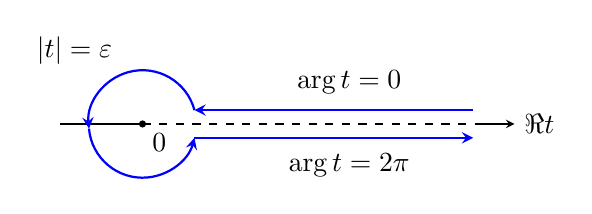
\begin{tikzpicture}[x=1.05cm,y=1.05cm,>=stealth]
\draw (-1,0)--(0,0);
\draw[dashed] (0,0)--(4.1,0);
\draw[->] (4.1,0)--(4.5,0) node[right] {$\Re t$};
\fill (0,0) circle (1.3pt) node[below right] {$0$};
\draw[blue,thick,->] (4,0.168)--(0.628,0.168);
\draw[blue,thick,->] (15:0.65) arc (15:185:0.65);
\draw[blue,thick,->] (185:0.65) arc (185:345:0.65);
\draw[blue,thick,->] (0.628,-0.168)--(4,-0.168);
\node[above] at (2.5,0.24) {$\arg t=0$};
\node[below] at (2.5,-0.24) {$\arg t=2\pi$};
\node[above left] at (-0.25,0.6) {$|t|=\varepsilon$};
\end{tikzpicture}
\end{center}
The two lips of the cut are displaced in the sketch for visibility.
Initially assume $\Re\nu>-1$.  On the upper lip $t=x$ with
$\arg t=0$, so $t^\nu=x^\nu$, but the direction is inward ($x$ runs
from $\infty$ to $\varepsilon$).  Its contribution is
\[
I_{\rm upper}=-e^{-\pi i\nu}
\int_\varepsilon^\infty e^{-x}x^\nu dx.
\]
On the lower lip the continuous argument is $2\pi$, so
$t^\nu=e^{2\pi i\nu}x^\nu$; since $e^{-\pi i\nu}e^{2\pi i\nu}
=e^{\pi i\nu}$, the outward contribution is
\[
I_{\rm lower}=e^{\pi i\nu}
\int_\varepsilon^\infty e^{-x}x^\nu dx.
\]
On the small circle put $t=\varepsilon e^{i\theta}$,
$0\le\theta\le2\pi$, so $dt=i\varepsilon e^{i\theta}d\theta$ and
$t^\nu=\varepsilon^\nu e^{i\nu\theta}$.  There $|e^{-t}|\le
e^\varepsilon$ and
$|e^{-\pi i\nu}t^\nu|=\varepsilon^{\Re\nu}e^{(\pi-\theta)\Im\nu}
\le\varepsilon^{\Re\nu}e^{\pi|\Im\nu|}$, and the circle has length
$2\pi\varepsilon$.  The circle integral is therefore at most
$2\pi e^{\pi|\Im\nu|}\varepsilon^{\Re\nu+1}e^\varepsilon$ in
magnitude, which tends to zero because $\Re\nu+1>0$.
The integrand is analytic in the plane cut along the positive real
axis, so by Cauchy's theorem $\int_C$ does not depend on
$\varepsilon$: for radii $\varepsilon_1<\varepsilon_2$ the two
contours differ by the boundary of the cut annulus
$\varepsilon_1<|t|<\varepsilon_2$ (the two circles and the lip
segments between them), which contains no singularity.  Hence
$\int_C$ is the limit as $\varepsilon\downarrow0$ of
$I_{\rm upper}+I_{\rm lower}$ plus the circle integral.  In this
limit the circle integral vanishes and the two ray integrals tend to
$\int_0^\infty e^{-x}x^\nu dx=\Gamma(\nu+1)$; with
$e^{\pi i\nu}-e^{-\pi i\nu}=2i\sin\pi\nu$,
\begin{align*}
\int_C e^{-t}e^{-\pi i\nu}t^\nu dt
&=(e^{\pi i\nu}-e^{-\pi i\nu})
 \int_0^\infty e^{-x}x^\nu dx\\
&=\boxed{2i\sin(\pi\nu)\Gamma(\nu+1)}.
\end{align*}

For $\Re\nu\le-1$, keep a nonzero circle radius; the individual
ray integrals cannot be extended to zero separately.  For fixed
$\varepsilon$ the complete contour integral is entire in $\nu$:
the circle is compact and the ray tails are dominated uniformly on
compact parameter sets by an exponential times a fixed power.
By the Cauchy argument above, which did not use $\Re\nu>-1$, it is
independent of $\varepsilon$.  Therefore the identity continues
analytically.  By the reflection formula,
$\Gamma(\nu+1)\Gamma(-\nu)=\pi/\sin\pi(\nu+1)=-\pi/\sin\pi\nu$, so its
left side is the entire function
\[
2i\Gamma(\nu+1)\sin\pi\nu=-\frac{2\pi i}{\Gamma(-\nu)}.
\]
\erratum{Only nonnegative integer $\nu$ makes the integrand entire
in $t$ and gives zero.  At negative integers the integral is nonzero;
the text's unqualified statement about integer $\nu$ needs this
restriction.}
Indeed, for $\nu=-m$, $m=1,2,\ldots$, the integrand is
$(-1)^m e^{-t}t^{-m}$.  Since $t^{-m}$ is single valued, the two lips
carry the same integrand in opposite directions and cancel, so only
the circle contributes.  The coefficient of $t^{-1}$ is
$(-1)^m(-1)^{m-1}/(m-1)!=-1/(m-1)!$, so by the residue theorem the
counterclockwise circle gives $2\pi i\cdot[-1/(m-1)!]=-2\pi i/(m-1)!$,
which is the continued formula $-2\pi i/\Gamma(-\nu)=-2\pi i/\Gamma(m)$.


\Needspace{9\baselineskip}
\subsection*{13.2 Digamma and Polygamma Functions}

\Needspace{5\baselineskip}
\par\bigskip
\noindent\textbf{13.2.1}\quad For ``small'' values of $x$,
\[
\ln\Gamma(x+1)=-\gamma x+\sum_{n=2}^{\infty}(-1)^{n}\frac{\zeta(n)}{n}x^{n},
\]
where $\gamma$ is the Euler-Mascheroni constant and $\zeta(n)$ the Riemann
zeta function. For what values of $x$ does this series converge?
\par\nobreak\hfill\emph{ANS.}\enspace $-1 < x\le1$.\par
Note that if $x=1$, we obtain
\[
\gamma=\sum_{n=2}^{\infty}(-1)^{n}\frac{\zeta(n)}{n},
\]
a series for the Euler-Mascheroni constant. The convergence of this series is
exceedingly slow. For actual computation of $\gamma$, other, indirect,
approaches are far superior (see Exercise 12.3.2).
\solution
Write $\zeta(n)=1+d_n$.  Since $k^{-n}\le\int_{k-1}^kt^{-n}dt$ for
$k\ge3$,
\[
0<d_n=\sum_{k=2}^{\infty}k^{-n}
\le 2^{-n}+\int_2^\infty t^{-n}dt
=2^{-n}+\frac{2^{1-n}}{n-1}
=2^{-n}\left(1+\frac2{n-1}\right).
\]
Thus, apart from the term $-\gamma x$, the series is the sum of
\[
\sum_{n=2}^\infty\frac{(-x)^n}n
\qquad\text{and}\qquad
\sum_{n=2}^\infty\frac{(-1)^nd_n}{n}x^n.
\]
The first has radius one.  The second, the correction, converges
absolutely for $|x|<2$, because $d_n/n\le3\cdot2^{-n}$ bounds its
terms by $3(|x|/2)^n$.  The sum converges absolutely for $|x|<1$.
At $x=1$ the first series is the convergent alternating harmonic
series, while at $x=-1$ it is the divergent harmonic tail
$\sum_{n\ge2}1/n$; the correction converges at both endpoints, so the
whole series converges at $x=1$ and diverges at $x=-1$.  For $|x|>1$
the terms $\zeta(n)x^n/n$ do not tend to zero, since $\zeta(n)>1$ and
$|x|^n/n\to\infty$.  Hence the real convergence set is exactly
\[
\boxed{-1<x\le1}.
\]
To identify the endpoint sum, let $x\uparrow1$ in the interior
identity.  By Abel's theorem the power series, which converges at
$x=1$, tends to its value there, while
$\ln\Gamma(1+x)\to\ln\Gamma(2)=\ln1=0$.  Hence
$0=-\gamma+\sum_{n\ge2}(-1)^n\zeta(n)/n$, that is,
\[
\gamma=\sum_{n=2}^{\infty}(-1)^n\frac{\zeta(n)}n.
\]
The leading $1/n$ behavior explains the slow convergence.  For
complex $x$, the same decomposition gives conditional convergence
on $|x|=1$ except at $x=-1$.


\Needspace{5\baselineskip}
\par\bigskip
\noindent\textbf{13.2.2}\quad Show that the series expansion of
$\ln\Gamma(x+1)$ (Exercise 13.2.1) may be written as
\begin{enumerate}
\item[(a)] $\ln\Gamma(x+1)=\dfrac{1}{2}\ln\left(\dfrac{\pi x}{\sin\pi x}\right)
  -\gamma x-\displaystyle\sum_{n=1}^{\infty}\frac{\zeta(2n+1)}{2n+1}x^{2n+1}$,
\item[(b)] $\ln\Gamma(x+1)=\dfrac{1}{2}\ln\left(\dfrac{\pi x}{\sin\pi x}\right)
  -\dfrac{1}{2}\ln\left(\dfrac{1+x}{1-x}\right)+(1-\gamma)x$\\[2pt]
  $\hfill-\displaystyle\sum_{n=1}^{\infty}
  \left[\zeta(2n+1)-1\right]\frac{x^{2n+1}}{2n+1}$.
\end{enumerate}
Determine the range of convergence of each of these expressions.
\solution
Use the real logarithm initially on $-1<x<1$ (with removable
quotients at $x=0$).  Split the original series into even and odd
powers:
\[
\ln\Gamma(1+x)=-\gamma x+
\sum_{n=1}^{\infty}\frac{\zeta(2n)x^{2n}}{2n}
-\sum_{n=1}^{\infty}\frac{\zeta(2n+1)x^{2n+1}}{2n+1}.
\]
Reflection and recurrence give
$\Gamma(1+x)\Gamma(1-x)=x\Gamma(x)\Gamma(1-x)=\pi x/\sin\pi x$.
Adding the series at $x$ and $-x$ cancels $-\gamma x$ and the odd
terms and doubles the even ones:
\[
\ln\frac{\pi x}{\sin\pi x}=\ln\Gamma(1+x)+\ln\Gamma(1-x)
=2\sum_{n=1}^{\infty}\frac{\zeta(2n)x^{2n}}{2n}.
\]
\textbf{(a)} Substituting half of this for the even series gives
exactly the first requested form.
Its remaining odd series has radius one; at $x=1$ its positive
terms behave as $1/(2n+1)$, and at $x=-1$ their negatives do.
It therefore converges for $\boxed{-1<x<1}$ only.  In particular,
the finite limit of the complete expression at $x=1$ requires
cancellation of divergent pieces; direct endpoint substitution
in the separated terms is invalid.

\textbf{(b)} Split $\zeta(2n+1)=1+[\zeta(2n+1)-1]$ and use
\[
\sum_{n=1}^{\infty}\frac{x^{2n+1}}{2n+1}
=\frac12\ln\frac{1+x}{1-x}-x.
\]
This follows by integrating the geometric series
$(1-t^2)^{-1}=\sum_{n\ge0}t^{2n}$ from zero to $x$, which gives
$\sum_{n\ge0}x^{2n+1}/(2n+1)=\int_0^xdt/(1-t^2)
=\frac12\ln[(1+x)/(1-x)]$, and removing the linear term.  Hence
\[
-\sum_{n=1}^{\infty}\frac{\zeta(2n+1)x^{2n+1}}{2n+1}
=-\frac12\ln\frac{1+x}{1-x}+x
-\sum_{n=1}^{\infty}\left[\zeta(2n+1)-1\right]\frac{x^{2n+1}}{2n+1},
\]
and inserting this in (a) produces the second displayed form, with
$-\gamma x+x=(1-\gamma)x$.
By the bounds $2^{-m}<\zeta(m)-1\le2^{-m}[1+2/(m-1)]$ (the lower one
is the first term of $d_m$, the upper one is from Exercise 13.2.1),
$2^{2n+1}[\zeta(2n+1)-1]\to1$, so the remaining
series has radius two.  At $x=\pm2$ its terms behave as
$\pm1/(2n+1)$, a signed harmonic tail, and it diverges.  Thus this
series alone converges on $\boxed{-2<x<2}$, but \erratum{the expression as written with
separate real logarithms has the domain $-1<x<1$.}
If those logarithms are first combined, their contribution is
\[
\frac12\ln\frac{\pi x(1-x)}{(1+x)\sin\pi x}.
\]
This has a removable limit $\tfrac12\ln(1/2)$ at $x=1$, because
$\sin\pi x=\sin\pi(1-x)\approx\pi(1-x)$ there, so the quotient tends
to $\pi/(2\pi)=1/2$.  It is real on $-1<x<2$, since for $1<x<2$ both
$1-x$ and $\sin\pi x$ are negative and the quotient stays positive.
Both sides of the combined identity are analytic on $-1<x<2$ and
agree on $-1<x<1$, so by the identity theorem (uniqueness of
analytic continuation) the combined form extends the identity across
$x=1$ to that larger interval.  This continuation
must be distinguished from the domain of the separate logarithms.


\Needspace{5\baselineskip}
\par\bigskip
\noindent\textbf{13.2.3}\quad Verify that for $n$, a positive integer, the
following two forms of the digamma function are equal to each other:
\[
\psi(n+1)=\sum_{j=1}^{n}\frac{1}{j}-\gamma
\quad\text{and}\quad
\psi(n+1)=\sum_{j=1}^{\infty}\frac{n}{j(n+j)}-\gamma.
\]
\solution
For a fixed positive integer $n$, partial fractions give
\[
\frac{n}{j(n+j)}=\frac1j-\frac1{j+n}.
\]
Sum only to a finite $N$ before canceling.  With
$H_N=\sum_{j=1}^N1/j$ and
$\sum_{j=1}^N1/(j+n)=\sum_{i=n+1}^{N+n}1/i=H_{N+n}-H_n$,
\begin{align*}
\sum_{j=1}^N\frac{n}{j(n+j)}
&=H_N-(H_{N+n}-H_n)\\
&=H_n-\sum_{j=N+1}^{N+n}\frac1j.
\end{align*}
The final sum lies between zero and $n/(N+1)$, hence tends to
zero as $N\to\infty$.  Therefore
\[
\boxed{\sum_{j=1}^{\infty}\frac{n}{j(n+j)}=H_n},
\qquad\psi(n+1)=H_n-\gamma,
\]
and the two representations agree.  This argument avoids
subtracting two divergent harmonic series separately.


\Needspace{5\baselineskip}
\par\bigskip
\noindent\textbf{13.2.4}\quad Show that $\psi(z+1)$ has the series expansion
\[
\psi(z+1)=-\gamma+\sum_{n=2}^{\infty}(-1)^{n}\zeta(n)z^{n-1}.
\]
\par\smallskip
\erratum{The expansion holds for $|z|<1$.}
\solution
On every closed disk $|z|\le r<1$, the Maclaurin series for
$\ln\Gamma(1+z)$, Eq.~(13.44), may be differentiated term by term.
Indeed, the derivative terms
$(d/dz)[(-1)^n\zeta(n)z^n/n]=(-1)^n\zeta(n)z^{n-1}$ have absolute
values at most $\zeta(2)r^{n-1}$ (since $\zeta(n)\le\zeta(2)$), whose
sum converges; by the Weierstrass M-test the differentiated series
converges uniformly on the disk, which justifies the term-by-term
differentiation.  Since
$\psi(1+z)=d\ln\Gamma(1+z)/dz$ and $(d/dz)(-\gamma z)=-\gamma$,
differentiation gives
\[
\boxed{\psi(1+z)=-\gamma+
\sum_{n=2}^{\infty}(-1)^n\zeta(n)z^{n-1}},
\qquad |z|<1.
\]
\erratum{The domain $|z|<1$ is needed: on $|z|=1$ the
summands have magnitudes $\zeta(n)\to1$, so none of that boundary
belongs to the convergence set.}  The closest pole of the
expanded function is at $z=-1$, consistent with radius one.


\Needspace{5\baselineskip}
\par\bigskip
\noindent\textbf{13.2.5}\quad For a power-series expansion of
$\ln\Gamma(z+1)$, AMS-55 (see Additional Readings for the reference) lists
\[
\ln\Gamma(z+1)=-\ln(1+z)+z(1-\gamma)
+\sum_{n=2}^{\infty}(-1)^{n}\left[\zeta(n)-1\right]\frac{z^{n}}{n}.
\]
\begin{enumerate}
\item[(a)] Show that this agrees with Eq.~(13.44) for $|z| < 1$.
\item[(b)] What is the range of convergence of this new expression?
\end{enumerate}
\solution
\textbf{(a)} For $|z|<1$,
\[
\ln(1+z)=z-\sum_{n=2}^{\infty}(-1)^n\frac{z^n}{n}.
\]
Add this to the series for $\ln\Gamma(1+z)$.  The linear
coefficients combine to $1-\gamma$, and for each $n\ge2$ the
coefficients $(-1)^n\zeta(n)/n$ and $-(-1)^n/n$ combine to
$(-1)^n[\zeta(n)-1]/n$, giving
\[
\ln\Gamma(1+z)+\ln(1+z)
=(1-\gamma)z+
\sum_{n=2}^{\infty}(-1)^n\frac{\zeta(n)-1}{n}z^n.
\]
Moving $\ln(1+z)$ to the right proves the claimed agreement.

\textbf{(b)} Set $e_n=\zeta(n)-1-2^{-n}=\sum_{k\ge3}k^{-n}$.  The
integral comparison of Exercise 13.2.1, now starting at $k=3$, gives
the estimate
\[
0<e_n\le3^{-n}+\int_3^\infty t^{-n}dt
=3^{-n}\left(1+\frac3{n-1}\right).
\]
Since $(-1)^n[\zeta(n)-1]z^n/n=(-z/2)^n/n+(-1)^ne_nz^n/n$, the new
series is $\sum_{n=2}^\infty(-z/2)^n/n$ plus a correction absolutely
convergent for $|z|<3$ (its terms are at most $4(|z|/3)^n$).  Thus
its radius is two; on $|z|=2$ it converges except at $z=-2$, by the
Dirichlet test for the leading series $\sum w^n/n$, $|w|=1$, $w\ne1$.
Its real convergence set is $\boxed{-2<z\le2}$.

\erratum{Convergence of the series is distinct from the domain
of the complete logarithmic identity: with ordinary real
logarithms that identity requires $z>-1$, and hence holds for
$-1<z\le2$.  It is undefined at $z=-1$.}
More precisely, since $\Gamma(2+z)=(1+z)\Gamma(1+z)$, part (a)
shows that the analytic series equals
$\ln\Gamma(2+z)-(1-\gamma)z$ for $|z|<1$.  The function
$\Gamma(2+z)$ has no zeros and its nearest pole is at $z=-2$, so
$\ln\Gamma(2+z)$, continued from zero, is analytic on $|z|<2$, as is
the series (radius two).  Agreeing on $|z|<1$, the two agree on the
whole disk $|z|<2$ by the identity theorem (uniqueness of analytic
continuation).  Subtracting $\ln(1+z)$ gives the requested
identity on a slit disk, for example
$|z|<2$ with $z\notin(-2,-1]$, using compatible analytic branches.
The endpoint $z=2$ follows by Abel's theorem and continuity.


\Needspace{5\baselineskip}
\par\bigskip
\noindent\textbf{13.2.6}\quad Show that
\[
\frac{1}{2}\ln\left(\frac{\pi z}{\sin\pi z}\right)
=\sum_{n=1}^{\infty}\frac{\zeta(2n)}{2n}z^{2n},\quad|z| < 1.
\]
\emph{Hint.}~Use Eqs.~(13.23) and \erratum{(13.44)}.
\solution
Write the expansion in Eq.~(13.44) at $z$ and $-z$ and add:
\begin{align*}
\ln\Gamma(1+z)+\ln\Gamma(1-z)
&=\sum_{k=2}^{\infty}\frac{(-1)^k\zeta(k)}k
 [z^k+(-z)^k]\\
&=2\sum_{n=1}^{\infty}\frac{\zeta(2n)}{2n}z^{2n}.
\end{align*}
The linear terms and all odd powers cancel.  Reflection,
$\Gamma(z)\Gamma(1-z)=\pi/\sin\pi z$, followed by
$z\Gamma(z)=\Gamma(1+z)$, gives
\[
\Gamma(1+z)\Gamma(1-z)=\frac{\pi z}{\sin\pi z}.
\]
In $|z|<1$ the quotient has no zero or pole, with value one at
zero.  Choose its analytic logarithm to vanish there.  The sum
of the two gamma logarithms has that same value and exponential,
so there is no additional $2\pi i$ constant.  Dividing by two gives
\[
\boxed{\frac12\ln\frac{\pi z}{\sin\pi z}
=\sum_{n=1}^{\infty}\frac{\zeta(2n)}{2n}z^{2n}},\qquad |z|<1.
\]
\erratum{The printed hint cites Eq.~(13.35); the published errata
(Instructor's Manual, 6 April 2012) replace it by Eq.~(13.44), the
Maclaurin series of $\ln\Gamma(1+z)$ used above.}


\Needspace{5\baselineskip}
\par\bigskip
\noindent\textbf{13.2.7}\quad Write out a Weierstrass infinite-product
definition of $\ln\Gamma(z+1)$. Without differentiating, show that this leads
directly to the Maclaurin expansion of $\ln\Gamma(z+1)$, Eq.~(13.44).
\solution
Weierstrass' product, after using $\Gamma(1+z)=z\Gamma(z)$, is
\[
\frac1{\Gamma(1+z)}=e^{\gamma z}
\prod_{k=1}^{\infty}\left(1+\frac zk\right)e^{-z/k}.
\]
Taking the analytic logarithm that is zero at $z=0$ gives
\[
\ln\Gamma(1+z)=-\gamma z+
\sum_{k=1}^{\infty}\left[\frac zk-\ln\left(1+\frac zk\right)\right].
\]
For $|z|<1$, expand each logarithm by
$\ln(1+w)=w-w^2/2+w^3/3-\cdots$ with $w=z/k$, $|w|<1$.  Its linear
term cancels:
\[
\frac zk-\ln\left(1+\frac zk\right)
=\sum_{n=2}^{\infty}\frac{(-1)^n z^n}{n k^n}.
\]
The double series is absolutely convergent, since summing over $k$
first gives $\zeta(n)|z|^n/n\le\zeta(2)|z|^n$ and
\[
\sum_{n=2}^{\infty}\sum_{k=1}^{\infty}
\frac{|z|^n}{n k^n}
\le\zeta(2)\sum_{n=2}^{\infty}|z|^n<\infty.
\]
Interchange the sums and identify $\sum_{k=1}^\infty k^{-n}$:
\[
\boxed{\ln\Gamma(1+z)=-\gamma z+
\sum_{n=2}^{\infty}(-1)^n\frac{\zeta(n)}n z^n}.
\]
No differentiation of the product was used.


\Needspace{5\baselineskip}
\par\bigskip
\noindent\textbf{13.2.8}\quad Derive the difference relation for the
polygamma function,
\[
\psi^{(m)}(z+2)=\psi^{(m)}(z+1)+(-1)^{m}\frac{m!}{(z+1)^{m+1}},
\quad m=0,1,2,\ldots.
\]
\solution
Differentiate $\Gamma(z+2)=(z+1)\Gamma(z+1)$ logarithmically
at regular arguments, i.e., differentiate
$\ln\Gamma(z+2)=\ln(z+1)+\ln\Gamma(z+1)$.  The result is
\[
\psi(z+2)=\frac1{z+1}+\psi(z+1).
\]
This already proves the case $m=0$.  For $m\ge1$, differentiate
this relation $m$ times, using $\psi^{(m)}=d^m\psi/dz^m$; the $m$th
derivative of the first term is
\[
\frac{d^m}{dz^m}(z+1)^{-1}
=(-1)(-2)\cdots(-m)(z+1)^{-m-1}
=\frac{(-1)^m m!}{(z+1)^{m+1}}.
\]
Hence
\[
\boxed{\psi^{(m)}(z+2)=\psi^{(m)}(z+1)
+\frac{(-1)^m m!}{(z+1)^{m+1}}},\qquad m=0,1,2,\ldots.
\]
These are identities of meromorphic functions; a displayed value
at a pole is not a finite number.  For integer positive arguments,
the formulas recursively reduce to the values at one.


\Needspace{5\baselineskip}
\par\bigskip
\noindent\textbf{13.2.9}\quad The Pochhammer symbol $(a)_{n}$ is defined (for
integral $n$) as
\[
(a)_{n}=a(a+1)\cdots(a+n-1),\quad(a)_{0}=1.
\]
\begin{enumerate}
\item[(a)] Express $(a)_{n}$ in terms of factorials.
\item[(b)] Find $(d/da)(a)_{n}$ in terms of $(a)_{n}$ and digamma functions.
\end{enumerate}
\par\nobreak\hfill\emph{ANS.}\enspace
$\dfrac{d}{da}(a)_{n}=(a)_{n}\left[\psi(a+n)-\psi(a)\right]$.
\begin{enumerate}
\item[(c)] Show that
  \[
  (a)_{n+k}=(a+n)_{k}\cdot(a)_{n}.
  \]
\end{enumerate}
\par\smallskip
\erratum{The finite-product indices $n,k$ are nonnegative integers. Products involving singular gamma or digamma factors are evaluated by their polynomial continuation.}
\solution
\erratum{The finite-product definition here uses nonnegative
integers $n$ and, in part (c), $k$.}
\textbf{(a)} Repeated gamma recurrence gives
$\Gamma(a+n)=(a+n-1)(a+n-2)\cdots a\,\Gamma(a)=(a)_n\Gamma(a)$,
so
\[
\boxed{(a)_n=\frac{\Gamma(a+n)}{\Gamma(a)}
=\frac{(a+n-1)!}{(a-1)!}}.
\]
The factorials have their generalized meaning.  The finite
product is a polynomial in $a$ and defines any removable value
of this quotient at gamma poles.

\textbf{(b)} At points where all factors are nonzero,
logarithmic differentiation of the finite product gives
\[
\frac{d}{da}(a)_n=(a)_n\sum_{j=0}^{n-1}\frac1{a+j}.
\]
Iterating $\psi(a+1)-\psi(a)=1/a$ (Exercise 13.2.8 with $m=0$)
identifies the finite sum by telescoping,
$\psi(a+n)-\psi(a)=\sum_{j=0}^{n-1}[\psi(a+j+1)-\psi(a+j)]
=\sum_{j=0}^{n-1}1/(a+j)$:
\[
\boxed{\frac{d}{da}(a)_n=(a)_n[\psi(a+n)-\psi(a)]}.
\]
The same result follows from (a):
$(d/da)[\Gamma(a+n)/\Gamma(a)]
=[\Gamma(a+n)/\Gamma(a)][\psi(a+n)-\psi(a)]$.
At exceptional arguments use the equivalent polynomial formula
\[
\frac{d}{da}(a)_n=
\sum_{j=0}^{n-1}\prod_{\substack{0\le\ell<n\\\ell\ne j}}(a+\ell).
\]
For example, at $a=-j$ with $0\le j<n$ only the term that omits the
vanishing factor $a+j$ survives, and its value is
\[
\prod_{\ell=0}^{j-1}(\ell-j)\prod_{\ell=j+1}^{n-1}(\ell-j)
=(-1)^jj!\,(n-1-j)!,
\]
even though the separated digamma factors have poles.  For $n=0$
the empty product is one and its derivative is zero.

\textbf{(c)} Split the product after its first $n$ factors:
\begin{align*}
(a)_{n+k}
&=\left[\prod_{j=0}^{n-1}(a+j)\right]
  \left[\prod_{j=n}^{n+k-1}(a+j)\right]\\
&=\boxed{(a)_n(a+n)_k}.
\end{align*}
This polynomial proof also includes zeros and empty products.


\Needspace{5\baselineskip}
\par\bigskip
\noindent\textbf{13.2.10}\quad Verify the following special values of the
$\psi$ form of the digamma and polygamma functions:
\[
\psi(1)=-\gamma,\quad\psi^{(1)}(1)=\zeta(2),\quad
\psi^{(2)}(1)=-2\zeta(3).
\]
\solution
Differentiating the Weierstrass form
$\ln\Gamma(1+z)=-\gamma z+\sum_k[z/k-\ln(1+z/k)]$ of
Exercise 13.2.7 term by term (each term has derivative
$1/k-1/(k+z)=z/[k(k+z)]$, and these converge locally uniformly
away from the poles) gives the convergent digamma representation
\[
\psi(1+z)=-\gamma+
\sum_{k=1}^{\infty}\left(\frac1k-\frac1{k+z}\right).
\]
Putting $z=0$ makes every term of the sum vanish, so
$\boxed{\psi(1)=-\gamma}$.
Differentiation on compact sets away from the poles, with
$(d/dz)(k+z)^{-1}=-(k+z)^{-2}$ and $(d/dz)(k+z)^{-2}=-2(k+z)^{-3}$,
gives
\[
\psi^{(1)}(1+z)=\sum_{k=1}^{\infty}\frac1{(k+z)^2},
\qquad
\psi^{(2)}(1+z)=-2\sum_{k=1}^{\infty}\frac1{(k+z)^3}.
\]
Both differentiated sums converge absolutely and locally
uniformly.  Therefore at $z=0$,
\[
\boxed{\psi^{(1)}(1)=\sum_{k=1}^{\infty}k^{-2}=\zeta(2)},
\qquad
\boxed{\psi^{(2)}(1)=-2\sum_{k=1}^{\infty}k^{-3}=-2\zeta(3)}.
\]


\Needspace{5\baselineskip}
\par\bigskip
\noindent\textbf{13.2.11}\quad Verify:
\begin{enumerate}
\item[(a)] $\displaystyle\int_{0}^{\infty}e^{-r}\ln r\,dr=-\gamma$.
\item[(b)] $\displaystyle\int_{0}^{\infty}re^{-r}\ln r\,dr=1-\gamma$.
\item[(c)] $\displaystyle\int_{0}^{\infty}r^{n}e^{-r}\ln r\,dr
  =(n-1)!+n\int_{0}^{\infty}r^{n-1}e^{-r}\ln r\,dr$,\quad$n=1,2,3,\ldots$.
\end{enumerate}
\emph{Hint.}~These may be verified by integration by parts, or by
differentiating the Euler integral formula for $\Gamma(n+1)$ with respect to
$n$.
\solution
For $s$ in a compact subset of $\Re s>0$, on which
$\Re s\ge\varepsilon$ for some $\varepsilon>0$, differentiation of
Euler's integral is justified by the integrable bounds
$r^{\varepsilon-1}|\ln r|$ near zero and a polynomial times
$e^{-r}|\ln r|$ at infinity.  Hence
\[
\Gamma'(s)=\int_0^\infty r^{s-1}e^{-r}\ln r\,dr
=\Gamma(s)\psi(s).
\]
\textbf{(a)} At $s=1$, $\Gamma(1)=1$ and $\psi(1)=-\gamma$,
so the integral is $\boxed{-\gamma}$.

\textbf{(c)} Write $I_n=\int_0^\infty r^ne^{-r}\ln r\,dr$.
For integers $n\ge1$, integrate by parts with
$u=r^n\ln r$, $dv=e^{-r}dr$, so that
$du=(nr^{n-1}\ln r+r^{n-1})dr$ and $v=-e^{-r}$.  Since
$r^n\ln r\to0$ at zero and the exponential removes the upper
boundary term, and since $\int_0^\infty r^{n-1}e^{-r}dr=\Gamma(n)
=(n-1)!$,
\begin{align*}
I_n&=\bigl[-r^ne^{-r}\ln r\bigr]_0^\infty
+\int_0^\infty e^{-r}(nr^{n-1}\ln r+r^{n-1})dr\\
&=\boxed{nI_{n-1}+(n-1)!}.
\end{align*}
\textbf{(b)} In particular, $I_1=I_0+0!=\boxed{1-\gamma}$.
The general closed form is $I_n=n!(H_n-\gamma)$, with the harmonic
numbers $H_n=\sum_{j=1}^n1/j$ of Exercise 13.2.3 and $H_0=0$, as is
checked by this recurrence and $I_0=-\gamma$: if
$I_{n-1}=(n-1)!(H_{n-1}-\gamma)$, then
$I_n=n!(H_{n-1}-\gamma)+n!/n=n!(H_n-\gamma)$.  It agrees with
$I_n=\Gamma'(n+1)=\Gamma(n+1)\psi(n+1)$ and Exercise 13.2.3.
Integration by parts at $n=0$ would have a divergent boundary term,
which is why part (a) was evaluated before using this recurrence.


\Needspace{5\baselineskip}
\par\bigskip
\noindent\textbf{13.2.12}\quad Dirac relativistic wave functions for hydrogen
involve factors such as $\Gamma[2(1-\alpha^{2}Z^{2})^{1/2}+1]$ where $\alpha$,
the fine structure constant, is \erratum{approximated here by $1/137$} and $Z$ is the atomic number. Expand
$\Gamma[2(1-\alpha^{2}Z^{2})^{1/2}+1]$ in a series of powers of
$\alpha^{2}Z^{2}$.
\solution
Let $q=\alpha^2Z^2$ and expand about $q=0$, using the square-root
branch that equals one there.  The binomial series
$\sqrt{1-q}=1-\frac q2-\frac{q^2}8-\frac{q^3}{16}+O(q^4)$ gives
\[
2\sqrt{1-q}+1=3+\delta,
\qquad\delta=-q-\frac{q^2}{4}-\frac{q^3}{8}+O(q^4).
\]
Set $p=\psi(3)$, $r=\psi^{(1)}(3)$ and $s=\psi^{(2)}(3)$.
The recurrence of Exercise 13.2.8, applied with $z=0$ and $z=1$,
gives $\psi^{(m)}(3)=\psi^{(m)}(1)+(-1)^mm!\,(1+2^{-m-1})$; with
the values at one from Exercise 13.2.10 this yields
\[
p=\frac32-\gamma,\qquad
r=\zeta(2)-1-\frac14=\zeta(2)-\frac54,
\qquad s=-2\zeta(3)+2+\frac14=\frac94-2\zeta(3).
\]
Differentiating $\Gamma'=\Gamma\psi$ and using $\Gamma'=\Gamma\psi$
again at each step gives
$\Gamma''=\Gamma'\psi+\Gamma\psi'=\Gamma(\psi^2+\psi')$ and
$\Gamma^{(3)}=\Gamma\psi(\psi^2+\psi')+\Gamma(2\psi\psi'+\psi'')$,
that is,
\[
\Gamma''=\Gamma(\psi^2+\psi'),\qquad
\Gamma^{(3)}=\Gamma(\psi^3+3\psi\psi'+\psi'').
\]
Since $\Gamma(3)=2$, Taylor expansion in $\delta$ is
\[
\Gamma(3+\delta)=2\left[1+p\delta+
\frac{p^2+r}{2}\delta^2+
\frac{p^3+3pr+s}{6}\delta^3+O(\delta^4)\right].
\]
Now $\delta^2=q^2+q^3/2+O(q^4)$ and
$\delta^3=-q^3+O(q^4)$.  Inside the brackets the coefficient of $q$
is $-p$; that of $q^2$ is $-p/4+(p^2+r)/2$; and that of $q^3$ is
$-p/8+(p^2+r)/4-(p^3+3pr+s)/6$.  Multiplying by two,
\begin{align*}
\Gamma(2\sqrt{1-q}+1)
={}&2-2pq+\left(p^2+r-\frac p2\right)q^2\\
&+\left[-\frac p4+\frac{p^2+r}{2}
-\frac{p^3+3pr+s}{3}\right]q^3+O(q^4).
\end{align*}
Here $-2p=2\gamma-3$ and
\[
p^2+r-\frac p2
=\left(\frac94-3\gamma+\gamma^2\right)+\zeta(2)-\frac54
-\frac34+\frac\gamma2
=\gamma^2-\frac52\gamma+\zeta(2)+\frac14.
\]
In particular, the first three terms in the original variables are
\[
\boxed{2+(2\gamma-3)\alpha^2Z^2+
\left[\gamma^2-\frac52\gamma+\zeta(2)+\frac14\right]
\alpha^4Z^4+O(\alpha^6Z^6)}.
\]
For the $q^3$ coefficient, multiplying out the products and adding
$s=\tfrac94-2\zeta(3)$ gives
\begin{align*}
p^3&=\frac{27}8-\frac{27}4\gamma+\frac92\gamma^2-\gamma^3,\qquad
3pr=\frac92\zeta(2)-\frac{45}8+\frac{15}4\gamma-3\gamma\zeta(2),\\
p^3+3pr+s&=-\gamma^3+\frac92\gamma^2-3\gamma-3\gamma\zeta(2)
+\frac92\zeta(2)-2\zeta(3),\\
-\frac p4+\frac{p^2+r}2&=\frac{\gamma^2}2-\frac54\gamma
+\frac{\zeta(2)}2+\frac18,
\end{align*}
and subtracting one third of the second line from the third gives the
$q^3$ coefficient
$\gamma^3/3-\gamma^2-\gamma/4+(\gamma-1)\zeta(2)+\tfrac23\zeta(3)
+\tfrac18$.  Numerically,
\[
\Gamma(2\sqrt{1-q}+1)=2-1.845569\,q+0.785073\,q^2-0.182458\,q^3
+O(q^4),
\]
which can be checked by evaluating the gamma function directly: at
$q=0.1$, $\Gamma(2\sqrt{0.9}+1)=\Gamma(2.8973666)=1.8231159$, while
the cubic gives $1.8231114$.  The difference, about
$4.5\times10^{-6}$, is the size of the omitted $q^4$ term: its
coefficient, obtained in the same way from $\Gamma^{(4)}$ and
$\psi^{(3)}(3)$, is $0.04416$, so the term is $4.4\times10^{-6}$ at
$q=0.1$.
Higher terms follow from the same two Taylor expansions.  The
expansion is local at $q=0$ and converges for $|q|<1$; there the
chosen square root has positive real part, so its gamma argument
encounters no gamma pole.  Physically, a short truncation requires
$\alpha^2Z^2$ small.  The value of $\alpha$ does not enter the
coefficients; the statement's $1/137$ approximates the measured
$\alpha\simeq1/137.036$.


\Needspace{5\baselineskip}
\par\bigskip
\noindent\textbf{13.2.13}\quad The quantum mechanical description of a
particle in a Coulomb field requires a knowledge of the argument of
$\Gamma(z)$ when $z$ is complex. Determine the argument of $\Gamma(1+ib)$
for small, real $b$.
\solution
Choose the argument continuously from $b=0$, where $\Gamma(1)=1$
and the argument is zero; it is then the imaginary part of the
logarithm of Eq.~(13.44), which vanishes at $z=0$.  For $|b|<1$,
substitute $z=ib$ in
\[
\ln\Gamma(1+z)=-\gamma z+
\sum_{n=2}^{\infty}(-1)^n\frac{\zeta(n)}n z^n.
\]
The linear term $-\gamma ib$ contributes $-\gamma b$ to the
imaginary part.  Even powers $(ib)^{2m}=(-1)^mb^{2m}$ are real.  For
the odd powers $n=2m+1$,
$(-1)^{2m+1}i^{2m+1}=-i\,(i^2)^m=(-1)^{m+1}i$.  Therefore
\[
\arg\Gamma(1+ib)=\Im\ln\Gamma(1+ib)
=-\gamma b+\sum_{m=1}^{\infty}(-1)^{m+1}
\frac{\zeta(2m+1)}{2m+1}b^{2m+1},
\]
that is,
\[
\boxed{\arg\Gamma(1+ib)
=-\gamma b+\frac{\zeta(3)}3b^3
-\frac{\zeta(5)}5b^5+\frac{\zeta(7)}7b^7-\cdots}.
\]
The leading approximation is $-\gamma b$, with an error of order
$b^3$.  This is the continuous local phase (and agrees with the
principal phase for sufficiently small $b$); arbitrary arguments
differ by $2\pi$ multiples.  Its oddness in $b$ also follows from
$\Gamma(1-ib)=\overline{\Gamma(1+ib)}$.


\Needspace{5\baselineskip}
\par\bigskip
\noindent\textbf{13.2.14}\quad Using digamma and polygamma functions, sum the
series
\begin{enumerate}
\item[(a)] $\displaystyle\sum_{n=1}^{\infty}\frac{1}{n(n+1)}$,\quad
(b) $\displaystyle\sum_{n=2}^{\infty}\frac{1}{n^{2}-1}$.
\end{enumerate}
\emph{Note.}~You can use Exercise 13.2.8 to calculate the needed digamma
functions.
\solution
Use the digamma identity
\[
\psi(1+z)+\gamma=\sum_{j=1}^{\infty}\frac{z}{j(j+z)},
\]
which is the representation of Exercise 13.2.10 with
$1/j-1/(j+z)=z/[j(j+z)]$.
\textbf{(a)} At $z=1$ the requested sum is
$\psi(2)+\gamma$.  The recurrence of Exercise 13.2.8 ($m=0$, $z=0$),
$\psi(2)=\psi(1)+1=-\gamma+1$, gives
\[
\boxed{\sum_{n=1}^{\infty}\frac1{n(n+1)}=1}.
\]
\textbf{(b)} Put $j=n-1$; then $n^2-1=(n-1)(n+1)=j(j+2)$.  At $z=2$
the identity gives $\sum_j2/[j(j+2)]=\psi(3)+\gamma$, and the
recurrence ($m=0$, $z=1$) gives $\psi(3)=\psi(2)+\tfrac12
=\tfrac32-\gamma$.  Hence
\begin{align*}
\sum_{n=2}^{\infty}\frac1{n^2-1}
&=\sum_{j=1}^{\infty}\frac1{j(j+2)}
=\frac12[\psi(3)+\gamma]\\
&=\frac12\left(1+\frac12\right)=\boxed{\frac34}.
\end{align*}
As a separate check, the partial fractions
$1/[n(n+1)]=1/n-1/(n+1)$ and
$1/(n^2-1)=\tfrac12[1/(n-1)-1/(n+1)]$ make the finite partial sums
telescope to $1-1/(N+1)$ in (a) and
$\tfrac12[1+1/2-1/N-1/(N+1)]$ in (b), respectively;
their limits give the same answers.


\Needspace{5\baselineskip}
\par\bigskip
\noindent\textbf{13.2.15}\quad Show that
\[
\sum_{n=1}^{\infty}\frac{1}{(n+a)(n+b)}
=\frac{1}{(b-a)}\left[\psi(1+b)-\psi(1+a)\right],
\]
where $a\neq b$, and neither $a$ nor $b$ is a negative integer. It is of some
interest to compare this summation with the corresponding integral,
\[
\int_{1}^{\infty}\frac{dx}{(x+a)(x+b)}
=\frac{1}{b-a}\left[\ln(1+b)-\ln(1+a)\right].
\]
The relation between $\psi(x)$ and $\ln x$ is made explicit in the analysis
leading to Stirling's formula.
\par\smallskip
\erratum{For the displayed ordinary real improper integral and real logarithms, require real $a,b>-1$ as well as $a\ne b$. The series has the wider domain stated above.}
\solution
For the stated admissible $a,b$, every denominator is nonzero
and the summands are $O(n^{-2})$, so the series converges
absolutely.  Subtract the two convergent digamma representations:
\begin{align*}
\psi(1+b)-\psi(1+a)
&=\sum_{n=1}^{\infty}
\left(\frac1{n+a}-\frac1{n+b}\right)\\
&=(b-a)\sum_{n=1}^{\infty}\frac1{(n+a)(n+b)}.
\end{align*}
Division by $b-a$ proves
\[
\boxed{\sum_{n=1}^{\infty}\frac1{(n+a)(n+b)}
=\frac{\psi(1+b)-\psi(1+a)}{b-a}}.
\]
The removable case $b=a$ is
$\sum_{n=1}^{\infty}(n+a)^{-2}=\psi^{(1)}(1+a)$.

\erratum{The accompanying real improper integral requires
stronger conditions, for example real $a,b>-1$.  Merely excluding
negative integers does not prevent an interior pole: $a=-3/2$,
$b=0$ gives one at $x=3/2$.}
Under $a,b>-1$, partial fractions give
\begin{align*}
\int_1^R\frac{dx}{(x+a)(x+b)}
&=\frac1{b-a}
\bigl[\ln(x+a)-\ln(x+b)\bigr]_1^R\\
&=\frac1{b-a}\left[\ln\frac{R+a}{R+b}
+\ln(1+b)-\ln(1+a)\right].
\end{align*}
The first logarithm tends to zero, proving the quoted integral.
When $b\to a>-1$, its value tends to $1/(1+a)$, whereas the
series tends to the trigamma value above.


\Needspace{9\baselineskip}
\subsection*{13.3 The Beta Function}

\Needspace{5\baselineskip}
\par\bigskip
\noindent\textbf{13.3.1}\quad Verify the following beta function identities:
\begin{enumerate}
\item[(a)] $B(a,b)=B(a+1,b)+B(a,b+1)$,
\item[(b)] $B(a,b)=\dfrac{a+b}{b}B(a,b+1)$,
\item[(c)] $B(a,b)=\dfrac{b-1}{a}B(a+1,b-1)$,
\item[(d)] $B(a,b)B(a+b,c)=B(b,c)B(a,b+c)$.
\end{enumerate}
\solution
Start where the beta integrals converge; in part (c) take
$\Re b>1$ as well as $\Re a>0$.  The results then extend as
meromorphic identities wherever the displayed values are defined.

\textbf{(a)} Insert $1=t+(1-t)$ into the defining integral:
\begin{align*}
B(a,b)&=\int_0^1 t^{a-1}(1-t)^{b-1}[t+(1-t)]dt\\
&=\boxed{B(a+1,b)+B(a,b+1)}.
\end{align*}
\textbf{(b)} Gamma recurrence gives
\[
B(a,b+1)=\frac{\Gamma(a)b\Gamma(b)}{(a+b)\Gamma(a+b)}
=\frac b{a+b}B(a,b),
\]
so $\boxed{B(a,b)=\dfrac{a+b}{b}B(a,b+1)}$.

\textbf{(c)} Use $\Gamma(a+1)=a\Gamma(a)$ and
$\Gamma(b-1)=\Gamma(b)/(b-1)$:
\[
B(a+1,b-1)=\frac{a\Gamma(a)\Gamma(b)}{(b-1)\Gamma(a+b)}
=\frac a{b-1}B(a,b).
\]
Rearranging gives the requested identity.  When one of the
separated factors has a pole, an equivalent continued identity
must be interpreted by a limit, not by multiplying undefined values.

\textbf{(d)} Multiplication cancels the intermediate gamma factor:
\begin{align*}
B(a,b)B(a+b,c)
&=\frac{\Gamma(a)\Gamma(b)}{\Gamma(a+b)}
  \frac{\Gamma(a+b)\Gamma(c)}{\Gamma(a+b+c)}\\
&=\frac{\Gamma(a)\Gamma(b)\Gamma(c)}{\Gamma(a+b+c)}\\
&=\frac{\Gamma(b)\Gamma(c)}{\Gamma(b+c)}
  \frac{\Gamma(a)\Gamma(b+c)}{\Gamma(a+b+c)}\\
&=\boxed{B(b,c)B(a,b+c)}.
\end{align*}


\Needspace{5\baselineskip}
\par\bigskip
\noindent\textbf{13.3.2}\quad
\begin{enumerate}
\item[(a)] Show that
  \[
  \int_{-1}^{1}(1-x^{2})^{1/2}x^{2n}\,dx=\begin{cases}
  \pi/2, & n=0\\[4pt]
  \pi\dfrac{(2n-1)!!}{(2n+2)!!}, & n=1,2,3,\ldots.
  \end{cases}
  \]
\item[(b)] Show that
  \[
  \int_{-1}^{1}(1-x^{2})^{-1/2}x^{2n}\,dx=\begin{cases}
  \pi, & n=0,\\[4pt]
  \pi\dfrac{(2n-1)!!}{(2n)!!}, & n=1,2,3,\ldots.
  \end{cases}
  \]
\end{enumerate}
\solution
Both integrands are even.  In twice the integral from zero to one,
put $u=x^2$, so $2\,dx=u^{-1/2}du$.
\textbf{(a)} This gives
\begin{align*}
\int_{-1}^1(1-x^2)^{1/2}x^{2n}dx
&=\int_0^1u^{n-1/2}(1-u)^{1/2}du\\
&=B\left(n+\frac12,\frac32\right)
=\frac{\Gamma(n+1/2)\Gamma(3/2)}{\Gamma(n+2)}\\
&=\frac{[(2n-1)!!\sqrt\pi/2^n](\sqrt\pi/2)}{(n+1)!}
=\boxed{\pi\frac{(2n-1)!!}{(2n+2)!!}}.
\end{align*}
Here $(2n+2)!!=2^{n+1}(n+1)!$.  With $(-1)!!=1$ this
includes $n=0$, giving $\pi/2$.

\textbf{(b)} The same substitution changes the second integral to
\begin{align*}
B\left(n+\frac12,\frac12\right)
&=\frac{\Gamma(n+1/2)\Gamma(1/2)}{\Gamma(n+1)}\\
&=\frac{(2n-1)!!\pi}{2^nn!}
=\boxed{\pi\frac{(2n-1)!!}{(2n)!!}}.
\end{align*}
This also includes $n=0$, because $0!!=1$.  The endpoint powers
$\pm1/2$ are greater than $-1$, so both improper integrals exist.


\Needspace{5\baselineskip}
\par\bigskip
\noindent\textbf{13.3.3}\quad Show that
\[
\int_{-1}^{1}(1-x^{2})^{n}\,dx=\frac{2(2n)!!}{(2n+1)!!},\quad n=0,1,2,\ldots.
\]
\solution
Evenness followed by $u=x^2$ yields
\[
\int_{-1}^1(1-x^2)^n dx
=2\int_0^1(1-x^2)^n dx
=\int_0^1u^{-1/2}(1-u)^n du
=B\left(\frac12,n+1\right).
\]
Now $\Gamma(n+3/2)=(2n+1)!!\sqrt\pi/2^{n+1}$, so
\[
B\left(\frac12,n+1\right)
=\frac{\sqrt\pi\,n!}{(2n+1)!!\sqrt\pi/2^{n+1}}
=\boxed{\frac{2(2n)!!}{(2n+1)!!}}.
\]
At $n=0$ this is two, the length of the interval, checking the
empty-product convention.


\Needspace{5\baselineskip}
\par\bigskip
\noindent\textbf{13.3.4}\quad Evaluate
$\displaystyle\int_{-1}^{1}(1+x)^{a}(1-x)^{b}\,dx$ in terms of the beta
function.
\par\nobreak\hfill\emph{ANS.}\enspace $2^{a+b+1}B(a+1,b+1)$.
\par\smallskip
\erratum{Require $\Re a,\Re b>-1$ for this improper integral.}
\solution
\erratum{The improper integral requires $\Re a>-1$ and
$\Re b>-1$; the bases inside the interval are positive.}
Put $u=(1+x)/2$, so $x=2u-1$, $dx=2du$,
$1+x=2u$ and $1-x=2(1-u)$.  The limits $x=-1,1$ become
$u=0,1$.  Therefore
\begin{align*}
\int_{-1}^1(1+x)^a(1-x)^b dx
&=2^{a+b+1}\int_0^1u^a(1-u)^bdu\\
&=\boxed{2^{a+b+1}B(a+1,b+1)}\\
&=2^{a+b+1}\frac{\Gamma(a+1)\Gamma(b+1)}{\Gamma(a+b+2)}.
\end{align*}
The factor $2^{a+b+1}$ includes the Jacobian two.  Outside the
stated convergence domain the gamma expression may continue
meromorphically, but that continuation is not the original
convergent improper integral.


\Needspace{5\baselineskip}
\par\bigskip
\noindent\textbf{13.3.5}\quad Show, by means of the beta function, that
\[
\int_{t}^{z}\frac{dx}{(z-x)^{1-\alpha}(x-t)^{\alpha}}
=\frac{\pi}{\sin\pi\alpha},\quad 0<\alpha<1.
\]
\par\smallskip
\erratum{Take real $t<z$.}
\solution
\erratum{Take real $t<z$ for the displayed real integral.}
Set $u=(x-t)/(z-t)$.  Then
\[
x-t=(z-t)u,\quad z-x=(z-t)(1-u),\quad dx=(z-t)du.
\]
The denominator has total power $(1-\alpha)+\alpha=1$, so
its factor $z-t$ cancels the Jacobian.  Hence
\begin{align*}
\int_t^z\frac{dx}{(z-x)^{1-\alpha}(x-t)^\alpha}
&=\int_0^1u^{-\alpha}(1-u)^{\alpha-1}du\\
&=B(1-\alpha,\alpha)
=\Gamma(1-\alpha)\Gamma(\alpha)\\
&=\boxed{\frac\pi{\sin\pi\alpha}}.
\end{align*}
The conditions $1-\alpha>0$ and $\alpha>0$ are exactly the
two endpoint convergence requirements.  Reflection gives the
last equality; the interval length has canceled completely.


\Needspace{5\baselineskip}
\par\bigskip
\noindent\textbf{13.3.6}\quad Show that the Dirichlet integral
\[
\iint x^{p}y^{q}\,dx\,dy=\frac{p!\,q!}{(p+q+2)!}=\frac{B(p+1,q+1)}{p+q+2},
\]
where the range of integration is the triangle bounded by the positive $x$-
and $y$-axes and the line $x+y=1$.
\par\smallskip
\erratum{The integral requires $\Re p,\Re q>-1$; factorials outside nonnegative integers mean gamma functions.}
\solution
\erratum{The integral converges for $\Re p,\Re q>-1$;
ordinary integer factorials correspond to $p,q\ge0$.}
Describe the triangle by $0\le x\le1$ and $0\le y\le1-x$.
Integrate with respect to $y$ first:
\begin{align*}
\int_0^1\int_0^{1-x}x^py^q\,dy\,dx
&=\frac1{q+1}\int_0^1x^p(1-x)^{q+1}dx\\
&=\frac{B(p+1,q+2)}{q+1}\\
&=\frac{\Gamma(p+1)\Gamma(q+2)}{(q+1)\Gamma(p+q+3)}\\
&=\boxed{\frac{\Gamma(p+1)\Gamma(q+1)}{\Gamma(p+q+3)}}.
\end{align*}
Since $\Gamma(q+2)=(q+1)\Gamma(q+1)$, the inner-integral
factor has canceled.  Recurrence in the remaining denominator
gives
\[
\frac{\Gamma(p+1)\Gamma(q+1)}{\Gamma(p+q+3)}
=\boxed{\frac{B(p+1,q+1)}{p+q+2}}
=\frac{p!q!}{(p+q+2)!}
\]
for nonnegative integers.  At $p=q=0$ the value is $1/2$, the
area of the triangle.


\Needspace{5\baselineskip}
\par\bigskip
\noindent\textbf{13.3.7}\quad Show that
\[
\int_{0}^{\infty}\!\!\int_{0}^{\infty}
e^{-(x^{2}+y^{2}+2xy\cos\theta)}\,dx\,dy=\frac{\theta}{2\sin\theta}.
\]
What are the limits on $\theta$?

\emph{Hint.}~Consider oblique $xy$-coordinates.
\par\nobreak\hfill\emph{ANS.}\enspace
\erratum{$-\pi<\theta<\pi$ for the unreduced formula, with value $1/2$ at $\theta=0$ by continuity. The integral itself converges for every real $\theta$ except odd multiples of $\pi$.}
\solution
First take $0<\theta<\pi$.  Introduce Cartesian variables
\[
X=x+y\cos\theta,\qquad Y=y\sin\theta.
\]
Then $X^2+Y^2=x^2+y^2+2xy\cos\theta$ and
$\partial(X,Y)/\partial(x,y)=\sin\theta>0$.  The original
positive quadrant maps onto the sector between the positive
$X$-axis ($y=0$) and the ray at angle $\theta$ ($x=0$).

\begin{center}
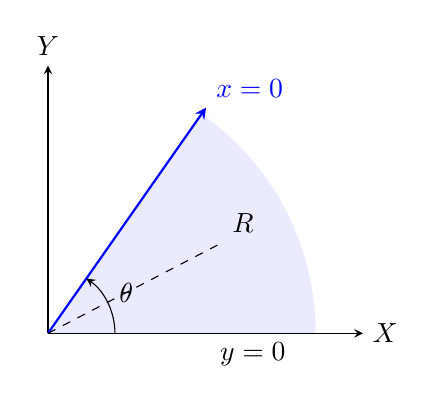
\begin{tikzpicture}[x=1cm,y=1cm,>=stealth]
\fill[blue!8] (0,0)--(3.4,0) arc (0:55:3.4)--cycle;
\draw[->] (0,0)--(4,0) node[right] {$X$};
\draw[->] (0,0)--(0,3.4) node[above] {$Y$};
\draw[thick,blue,->] (0,0)--(55:3.5) node[above right] {$x=0$};
\node[below] at (2.6,0) {$y=0$};
\draw[->] (0.85,0) arc (0:55:0.85);
\node at (27.5:1.12) {$\theta$};
\draw[dashed] (0,0)--(27.5:2.5) node[above right] {$R$};
\end{tikzpicture}
\end{center}
In polar coordinates $X=R\cos\phi$, $Y=R\sin\phi$,
\begin{align*}
I(\theta)&=\frac1{\sin\theta}
\int_0^\theta d\phi\int_0^\infty e^{-R^2}R\,dR\\
&=\frac\theta{\sin\theta}
\left[-\frac12e^{-R^2}\right]_0^\infty
=\boxed{\frac\theta{2\sin\theta}}.
\end{align*}
Both the original integral and this quotient are even in $\theta$,
so the result extends to $-\pi<\theta<0$.  At zero use
$u=x+y$, $v=x$, where $0\le v\le u$:
\[
I(0)=\int_0^\infty e^{-u^2}\int_0^u dv\,du
=\int_0^\infty ue^{-u^2}du=\frac12,
\]
the removable limit of the formula.

\erratum{The stated interval $-\pi<\theta<\pi$ is the range
for the unreduced formula $\theta/(2\sin\theta)$, including its
removable value at zero.  For unrestricted real $\theta$, the
integral is periodic and converges except at odd multiples of
$\pi$.}
Indeed, if $c=\cos\theta>-1$, the quadratic form on $x,y\ge0$
is at least $\min(1,1+c)(x^2+y^2)$, so a convergent Gaussian
dominates it.  If $c=-1$, the integrand is $e^{-(x-y)^2}$;
on $x\ge1$, $x\le y\le x+1$ it is at least $e^{-1}$, giving
infinite integral.  In general reduce to
$\vartheta=\arccos(\cos\theta)\in[0,\pi]$ and use
$\vartheta/(2\sin\vartheta)$, with the endpoint conventions just
established.


\Needspace{5\baselineskip}
\par\bigskip
\noindent\textbf{13.3.8}\quad Evaluate (using the beta function)
\begin{enumerate}
\item[(a)] $\displaystyle\int_{0}^{\pi/2}\cos^{1/2}\theta\,d\theta
  =\frac{(2\pi)^{3/2}}{16[\Gamma(5/4)]^{2}}$,
\item[(b)] $\displaystyle\int_{0}^{\pi/2}\cos^{n}\theta\,d\theta
  =\int_{0}^{\pi/2}\sin^{n}\theta\,d\theta
  =\frac{\sqrt{\pi}\,[(n-1)/2]!}{2(n/2)!}$\\[4pt]
  $\hfill=\begin{cases}
  \dfrac{(n-1)!!}{n!!} & \text{for }n\text{ odd},\\[8pt]
  \dfrac{\pi}{2}\cdot\dfrac{(n-1)!!}{n!!} & \text{for }n\text{ even}.
  \end{cases}$
\end{enumerate}
\par\smallskip
\erratum{The general integral requires $\Re n>-1$; its odd/even forms use nonnegative integer $n$ and $(-1)!!=0!!=1$.}
\solution
For $u=\sin^2\theta$, the limits become zero and one and
\[
du=2\sin\theta\cos\theta\,d\theta,\qquad
d\theta=\frac{du}{2\sqrt{u(1-u)}},\qquad
\cos^n\theta=(1-u)^{n/2}.
\]
Thus the common form is
\[
I_n=\int_0^{\pi/2}\cos^n\theta\,d\theta
=\frac12\int_0^1u^{-1/2}(1-u)^{(n-1)/2}du
=\frac{\sqrt\pi\,\Gamma((n+1)/2)}{2\Gamma((n+2)/2)}.
\]
\erratum{This integral formula requires $\Re n>-1$; the odd/even
factorial forms below use nonnegative integer $n$.}
Replacing $\theta$ by $\pi/2-\theta$ proves the same value for
$\int_0^{\pi/2}\sin^n\theta\,d\theta$.

\textbf{(a)} At $n=1/2$,
$I_{1/2}=\sqrt\pi\,\Gamma(3/4)/[2\Gamma(5/4)]$.
Reflection and recurrence give
\[
\Gamma(1/4)\Gamma(3/4)=\pi\sqrt2,
\qquad\Gamma(1/4)=4\Gamma(5/4).
\]
Thus
\[
\boxed{I_{1/2}=\frac{\pi\sqrt{2\pi}}{8[\Gamma(5/4)]^2}
=\frac{(2\pi)^{3/2}}{16[\Gamma(5/4)]^2}}.
\]
\textbf{(b)} The gamma expression is precisely
$\sqrt\pi\,[(n-1)/2]!/[2(n/2)!]$.  For $n=2m+1$,
\[
I_{2m+1}=\frac{\sqrt\pi\,m!}{2\Gamma(m+3/2)}
=\frac{2^mm!}{(2m+1)!!}
=\boxed{\frac{(2m)!!}{(2m+1)!!}}.
\]
For $n=2m$,
\[
I_{2m}=\frac{\sqrt\pi\,\Gamma(m+1/2)}{2m!}
=\frac\pi2\frac{(2m-1)!!}{2^mm!}
=\boxed{\frac\pi2\frac{(2m-1)!!}{(2m)!!}}.
\]
The case $m=0$ in the even formula gives $I_0=\pi/2$.


\Needspace{5\baselineskip}
\par\bigskip
\noindent\textbf{13.3.9}\quad Evaluate
$\displaystyle\int_{0}^{1}(1-x^{4})^{-1/2}\,dx$ as a beta function.
\par\nobreak\hfill\emph{ANS.}\enspace
$\dfrac{[\Gamma(5/4)]^{2}\cdot4}{(2\pi)^{1/2}}=1.311028777$.
\solution
Put $u=x^4$, so $dx=\tfrac14u^{-3/4}du$.  The endpoint
exponents $-3/4$ and $-1/2$ are both integrable, and
\[
I=\frac14\int_0^1u^{-3/4}(1-u)^{-1/2}du
=\boxed{\frac14B\left(\frac14,\frac12\right)}
=\frac{\Gamma(1/4)\sqrt\pi}{4\Gamma(3/4)}.
\]
Use $\Gamma(1/4)\Gamma(3/4)=\pi\sqrt2$ to remove
$\Gamma(3/4)$, then $\Gamma(1/4)=4\Gamma(5/4)$:
\[
I=\frac{[\Gamma(1/4)]^2}{4\sqrt{2\pi}}
=\boxed{\frac{4[\Gamma(5/4)]^2}{\sqrt{2\pi}}}
=1.311028777146\ldots.
\]
For an independent numerical quadrature one can also put
$x=\sin\phi$; cancellation of $\cos\phi$ gives the nonsingular
integral $\int_0^{\pi/2}(1+\sin^2\phi)^{-1/2}d\phi$.


\Needspace{5\baselineskip}
\par\bigskip
\noindent\textbf{13.3.10}\quad Using beta functions, show that the integral
representation
\[
J_{\nu}(z)=\frac{2}{\pi^{1/2}\Gamma(\nu+\frac{1}{2})}
\left(\frac{z}{2}\right)^{\nu}
\int_{0}^{\pi/2}\sin^{2\nu}\theta\cos(z\cos\theta)\,d\theta,
\quad\Re(\nu)>-\tfrac{1}{2},
\]
reduces to the Bessel series
\[
J_{\nu}(z)=\sum_{s=0}^{\infty}(-1)^{s}
\frac{1}{s!\,\Gamma(s+\nu+1)}\left(\frac{z}{2}\right)^{2s+\nu},
\]
thereby confirming its validity.
\solution
Expand the cosine, keeping the same branch of $(z/2)^\nu$
throughout:
\[
\cos(z\cos\theta)=\sum_{s=0}^{\infty}
\frac{(-1)^s z^{2s}\cos^{2s}\theta}{(2s)!}.
\]
For fixed $z$, the absolute sum is bounded by $e^{|z|}$.
The remaining weight has magnitude $\sin^{2\Re\nu}\theta$,
which is integrable at zero exactly when $\Re\nu>-1/2$.
Dominated convergence therefore permits integration term by term.
The beta integral for each term is
\[
\int_0^{\pi/2}\sin^{2\nu}\theta\cos^{2s}\theta\,d\theta
=\frac12B\left(\nu+\frac12,s+\frac12\right)
=\frac{\Gamma(\nu+1/2)\Gamma(s+1/2)}{2\Gamma(s+\nu+1)}.
\]
Insert this in the proposed representation and cancel its
$2$ and $\Gamma(\nu+1/2)$ factors:
\[
J_\nu(z)=\left(\frac z2\right)^\nu
\sum_{s=0}^{\infty}\frac{(-1)^sz^{2s}}{\sqrt\pi(2s)!}
\frac{\Gamma(s+1/2)}{\Gamma(s+\nu+1)}.
\]
Finally,
\[
\Gamma\left(s+\frac12\right)
=\frac{(2s)!\sqrt\pi}{4^ss!},
\qquad
\frac{\Gamma(s+1/2)}{\sqrt\pi(2s)!}=\frac1{4^ss!}.
\]
Thus
\[
\boxed{J_\nu(z)=\sum_{s=0}^{\infty}
\frac{(-1)^s}{s!\Gamma(s+\nu+1)}
\left(\frac z2\right)^{2s+\nu}},
\]
the defining Bessel series.  For noninteger $\nu$ both
representations use a chosen branch of $z^\nu$; a value at zero
is taken only when the corresponding limit exists.


\Needspace{5\baselineskip}
\par\bigskip
\noindent\textbf{13.3.11}\quad Given the associated Legendre function, defined
in Chapter 15,
\[
P_{m}^{m}(x)=(2m-1)!!\,(1-x^{2})^{m/2},
\]
show that
\begin{enumerate}
\item[(a)] $\displaystyle\int_{-1}^{1}[P_{m}^{m}(x)]^{2}\,dx
  =\frac{2}{2m+1}(2m)!$,\quad$m=0,1,2,\ldots$,
\item[(b)] $\displaystyle\int_{-1}^{1}[P_{m}^{m}(x)]^{2}\frac{dx}{1-x^{2}}
  =2\cdot(2m-1)!$,\quad$m=1,2,3,\ldots$.
\end{enumerate}
\solution
Square the stated expression:
$[P_m^m(x)]^2=[(2m-1)!!]^2(1-x^2)^m$.
\textbf{(a)} Exercise 13.3.3 gives
\begin{align*}
\int_{-1}^1[P_m^m(x)]^2dx
&=[(2m-1)!!]^2\frac{2(2m)!!}{(2m+1)!!}\\
&=\frac{2(2m-1)!!(2m)!!}{2m+1}
=\boxed{\frac{2(2m)!}{2m+1}}.
\end{align*}
We used $(2m+1)!!=(2m+1)(2m-1)!!$ and
$(2m-1)!!(2m)!!=(2m)!$.  The case $m=0$ gives two.

\textbf{(b)} Division by $1-x^2$ reduces the exponent to $m-1$.
For $m\ge1$ the same beta evaluation yields
\begin{align*}
\int_{-1}^1[P_m^m(x)]^2\frac{dx}{1-x^2}
&=[(2m-1)!!]^2\frac{2(2m-2)!!}{(2m-1)!!}\\
&=2(2m-1)!!(2m-2)!!
=\boxed{2(2m-1)!}.
\end{align*}
At $m=0$ the second integral diverges at both endpoints,
explaining its different lower limit on $m$.  An alternative
associated-Legendre convention introduces $(-1)^m$, which has
no effect on either squared integral.


\Needspace{5\baselineskip}
\par\bigskip
\noindent\textbf{13.3.12}\quad Show that, for integers $p$ and $q$,
\begin{enumerate}
\item[(a)] $\displaystyle\int_{0}^{1}x^{2p+1}(1-x^{2})^{-1/2}\,dx
  =\frac{(2p)!!}{(2p+1)!!}$,
\item[(b)] $\displaystyle\int_{0}^{1}x^{2p}(1-x^{2})^{q}\,dx
  =\frac{(2p-1)!!\,(2q)!!}{(2p+2q+1)!!}$.
\end{enumerate}
\par\smallskip
\erratum{Take $p\ge0$ in (a), and $p,q\ge0$ in (b).}
\solution
\erratum{For the stated integer parameters, require $p\ge0$
in (a), and $p,q\ge0$ in (b).  Negative integer values produce
nonintegrable endpoint powers.}
Use $u=x^2$, $dx=du/(2\sqrt u)$.
\textbf{(a)} Since $x^{2p+1}dx=u^pdu/2$,
\begin{align*}
\int_0^1x^{2p+1}(1-x^2)^{-1/2}dx
&=\frac12 B\left(p+1,\frac12\right)
=\frac{p!\sqrt\pi}{2\Gamma(p+3/2)}\\
&=\frac{p!\sqrt\pi\,2^{p+1}}{2(2p+1)!!\sqrt\pi}
=\boxed{\frac{(2p)!!}{(2p+1)!!}}.
\end{align*}
\textbf{(b)} Here $x^{2p}dx=u^{p-1/2}du/2$, so
\begin{align*}
\int_0^1x^{2p}(1-x^2)^qdx
&=\frac12 B\left(p+\frac12,q+1\right)
=\frac{\Gamma(p+1/2)q!}{2\Gamma(p+q+3/2)}\\
&=\frac{[(2p-1)!!\sqrt\pi/2^p]q!}
 {2[(2p+2q+1)!!\sqrt\pi/2^{p+q+1}]}\\
&=\boxed{\frac{(2p-1)!!(2q)!!}{(2p+2q+1)!!}}.
\end{align*}
These formulas include $p=0$ or $q=0$ with the usual empty
products $(-1)!!=0!!=1$.


\Needspace{5\baselineskip}
\par\bigskip
\noindent\textbf{13.3.13}\quad A particle of mass $m$ moving in a symmetric
potential that is well described by $V(x)=A|x|^{n}$ has a total energy
$\frac{1}{2}m(dx/dt)^{2}+V(x)=E$. Solving for $dx/dt$ and integrating we find
that the period of motion is
\[
\tau=2\sqrt{2m}\int_{0}^{x_{\max}}\frac{dx}{(E-Ax^{n})^{1/2}},
\]
where $x_{\max}$ is a classical turning point given by
$Ax_{\max}^{n}=E$. Show that
\[
\tau=\frac{2}{n}\sqrt{\frac{2\pi m}{E}}
\left(\frac{E}{A}\right)^{1/n}
\frac{\Gamma(1/n)}{\Gamma(1/n+\frac{1}{2})}.
\]
\par\smallskip
\erratum{Assume $m,A,E,n>0$.}
\solution
\erratum{For the bounded oscillation considered here, take
$m,A,E>0$ and $n>0$.}
The positive turning point is $x_{\max}=(E/A)^{1/n}$.
On the outward quarter-cycle, energy conservation gives
\[
\frac{dx}{dt}=\sqrt{\frac2m}\sqrt{E-Ax^n},
\qquad
\frac\tau4=\sqrt{\frac m2}\int_0^{x_{\max}}
\frac{dx}{\sqrt{E-Ax^n}},
\]
which explains the factor in the question.  Set
$u=Ax^n/E=(x/x_{\max})^n$.  Then
\[
x=x_{\max}u^{1/n},\quad
 dx=\frac{x_{\max}}n u^{1/n-1}du,\quad
(E-Ax^n)^{-1/2}=E^{-1/2}(1-u)^{-1/2}.
\]
Both endpoints become zero and one, respectively.  Consequently
\begin{align*}
\tau&=\frac2n\sqrt{\frac{2m}E}\left(\frac EA\right)^{1/n}
\int_0^1u^{1/n-1}(1-u)^{-1/2}du\\
&=\frac2n\sqrt{\frac{2m}E}\left(\frac EA\right)^{1/n}
B\left(\frac1n,\frac12\right)\\
&=\boxed{\frac2n\sqrt{\frac{2\pi m}E}\left(\frac EA\right)^{1/n}
\frac{\Gamma(1/n)}{\Gamma(1/n+1/2)}}.
\end{align*}
As a check, $n=2$ and $A=m\omega^2/2$ give
$\tau=\pi\sqrt{2m/A}=2\pi/\omega$, the harmonic-oscillator
period, independent of $E$.


\Needspace{5\baselineskip}
\par\bigskip
\noindent\textbf{13.3.14}\quad Referring to Exercise 13.3.13,
\begin{enumerate}
\item[(a)] Determine the limit as $n\to\infty$ of
  \[
  \frac{2}{n}\sqrt{\frac{2\pi m}{E}}\left(\frac{E}{A}\right)^{1/n}
  \frac{\Gamma(1/n)}{\Gamma(1/n+\frac{1}{2})}.
  \]
\item[(b)] Find $\lim_{n\to\infty}\tau$ from the behavior of the integrand
  $(E-Ax^{n})^{-1/2}$.
\item[(c)] Investigate the behavior of the physical system (potential well)
  as $n\to\infty$. Obtain the period from inspection of this limiting
  physical system.
\end{enumerate}
\par\smallskip
\erratum{For a dimensionful family, write $V_n(x)=A(|x|/L)^n$ with fixed $A,L>0$; the displayed formula uses length units $L=1$.}
\solution
\textbf{(a)} Use the recurrence before taking the limit:
\[
\frac{\Gamma(1/n)}{n\Gamma(1/n+1/2)}
=\frac{\Gamma(1+1/n)}{\Gamma(1/n+1/2)}
\longrightarrow\frac{\Gamma(1)}{\Gamma(1/2)}=\frac1{\sqrt\pi}.
\]
Also $(E/A)^{1/n}\to1$ for fixed positive numerical $E/A$.
Hence the period written in the question tends to
\[
\boxed{\tau_\infty=2\sqrt{\frac{2m}E}}.
\]
\erratum{When comparing dimensionful potentials at different
$n$, fix a length $L$ and write $V_n(x)=A(|x|/L)^n$ with fixed
energy scale $A$.  The question uses length units with $L=1$;
the dimensionful limiting period is $2L\sqrt{2m/E}$.}

\textbf{(b)} To justify passing to the limit despite the moving
turning point, set $x=x_{\max}u$:
\[
\tau_n=2\sqrt{\frac{2m}E}\,x_{\max}
\int_0^1(1-u^n)^{-1/2}du.
\]
For $0\le u<1$, this integrand tends to one.  For $n\ge1$,
$u^n\le u$, so
\[
0<(1-u^n)^{-1/2}\le(1-u)^{-1/2},
\qquad\int_0^1(1-u)^{-1/2}du=2.
\]
Dominated convergence gives an integral limit of one, and
$x_{\max}=L(E/A)^{1/n}\to L$.  This proves the same limit
without ignoring the endpoint singularity.

\textbf{(c)} For $|x|<L$, $V_n(x)\to0$; for $|x|>L$,
$V_n(x)\to\infty$.  The limiting motion is free flight between
reflecting walls at $\pm L$, with speed $v=\sqrt{2E/m}$.
A round trip covers distance $4L$, so
\[
\boxed{\tau_\infty=\frac{4L}{v}=2L\sqrt{\frac{2m}E}}.
\]
The isolated value $V_n(\pm L)=A$ does not affect the limiting
travel time derived in (b).


\Needspace{5\baselineskip}
\par\bigskip
\noindent\textbf{13.3.15}\quad Show that
\[
\int_{0}^{\infty}\frac{\sinh^{\alpha}x}{\cosh^{\beta}x}\,dx
=\frac{1}{2}B\left(\frac{\alpha+1}{2},\frac{\beta-\alpha}{2}\right),
\quad-1<\alpha<\beta.
\]
\emph{Hint.}~Let $\sinh^{2}x=u$.
\solution
The endpoint behavior explains the given restrictions: near zero
$\sinh^\alpha x/\cosh^\beta x\sim x^\alpha$, whereas at infinity
it is asymptotic to $2^{\beta-\alpha}e^{(\alpha-\beta)x}$.
Thus for real parameters convergence requires $\alpha>-1$ and
$\beta>\alpha$.

Set $u=\sinh^2x$.  Since $\cosh^2x=1+u$,
\[
du=2\sinh x\cosh x\,dx=2\sqrt{u(1+u)}\,dx.
\]
It follows that
\begin{align*}
\int_0^\infty\frac{\sinh^\alpha x}{\cosh^\beta x}dx
&=\frac12\int_0^\infty
u^{(\alpha-1)/2}(1+u)^{-(\beta+1)/2}du.
\end{align*}
To recognize the beta integral, put $v=u/(1+u)$,
$du=dv/(1-v)^2$.  In general this shows
\[
\int_0^\infty u^{p-1}(1+u)^{-p-q}du
=\int_0^1v^{p-1}(1-v)^{q-1}dv=B(p,q).
\]
Here $p=(\alpha+1)/2$, $q=(\beta-\alpha)/2$, both positive.
Therefore
\[
\boxed{\int_0^\infty\frac{\sinh^\alpha x}{\cosh^\beta x}dx
=\frac12 B\left(\frac{\alpha+1}2,\frac{\beta-\alpha}2\right)}.
\]
For complex parameters the corresponding absolute-convergence
conditions are $\Re\alpha>-1$ and $\Re(\beta-\alpha)>0$.


\Needspace{5\baselineskip}
\par\bigskip
\noindent\textbf{13.3.16}\quad The beta distribution of probability theory has
a probability density
\[
f(x)=\frac{\Gamma(\alpha+\beta)}{\Gamma(\alpha)\Gamma(\beta)}
x^{\alpha-1}(1-x)^{\beta-1},
\]
with $x$ restricted to the interval $(0,1)$. Show that
\begin{enumerate}
\item[(a)] $\langle x\rangle$, the mean value, is
  $\dfrac{\alpha}{\alpha+\beta}$.
\item[(b)] $\sigma^{2}$, its variance, is
  $\langle x^{2}\rangle-\langle x\rangle^{2}
  =\dfrac{\alpha\beta}{(\alpha+\beta)^{2}(\alpha+\beta+1)}$.
\end{enumerate}
\par\smallskip
\erratum{Assume real $\alpha,\beta>0$.}
\solution
\erratum{A beta probability density requires real
$\alpha,\beta>0$.}
Its prefactor is $1/B(\alpha,\beta)$.  Consequently
\[
\langle x^q\rangle
=\frac{B(\alpha+q,\beta)}{B(\alpha,\beta)}
=\frac{\Gamma(\alpha+q)\Gamma(\alpha+\beta)}
{\Gamma(\alpha)\Gamma(\alpha+\beta+q)},
\qquad\Re q>-\alpha.
\]
At $q=0$ this equals one and verifies normalization.
\textbf{(a)} For $q=1$, apply gamma recurrence to numerator and
denominator:
\[
\langle x\rangle
=\frac{[\alpha\Gamma(\alpha)]\Gamma(\alpha+\beta)}
{\Gamma(\alpha)[(\alpha+\beta)\Gamma(\alpha+\beta)]}
=\boxed{\frac\alpha{\alpha+\beta}}.
\]
\textbf{(b)} For $q=2$ the same cancellation gives
\[
\langle x^2\rangle
=\frac{\alpha(\alpha+1)\Gamma(\alpha)\Gamma(\alpha+\beta)}
{\Gamma(\alpha)(\alpha+\beta)(\alpha+\beta+1)\Gamma(\alpha+\beta)}
=\frac{\alpha(\alpha+1)}{(\alpha+\beta)(\alpha+\beta+1)}.
\]
Subtract the squared mean using a common denominator:
\begin{align*}
\sigma^2&=\frac{\alpha(\alpha+1)(\alpha+\beta)
-\alpha^2(\alpha+\beta+1)}{(\alpha+\beta)^2(\alpha+\beta+1)}\\
&=\frac{\alpha[(\alpha^2+\alpha\beta+\alpha+\beta)
-(\alpha^2+\alpha\beta+\alpha)]}
{(\alpha+\beta)^2(\alpha+\beta+1)}\\
&=\boxed{\frac{\alpha\beta}{(\alpha+\beta)^2(\alpha+\beta+1)}}.
\end{align*}


\Needspace{5\baselineskip}
\par\bigskip
\noindent\textbf{13.3.17}\quad From
\[
\lim_{n\to\infty}
\frac{\displaystyle\int_{0}^{\pi/2}\sin^{2n}\theta\,d\theta}
{\displaystyle\int_{0}^{\pi/2}\sin^{2n+1}\theta\,d\theta}=1,
\]
derive the Wallis formula for $\pi$:
\[
\frac{\pi}{2}=\frac{2\cdot2}{1\cdot3}\cdot\frac{4\cdot4}{3\cdot5}
\cdot\frac{6\cdot6}{5\cdot7}\cdots.
\]
\solution
Write $I_k=\int_0^{\pi/2}\sin^k\theta\,d\theta$.
Exercise 13.3.8 gives
\[
I_{2n}=\frac\pi2\frac{(2n-1)!!}{(2n)!!},
\qquad I_{2n+1}=\frac{(2n)!!}{(2n+1)!!}.
\]
Therefore
\[
\frac{I_{2n}}{I_{2n+1}}
=\frac\pi2\frac{(2n-1)!!(2n+1)!!}{[(2n)!!]^2}.
\]
Define the finite product
\[
P_n=\prod_{j=1}^n\frac{(2j)^2}{(2j-1)(2j+1)}
=\frac{[(2n)!!]^2}{(2n-1)!!(2n+1)!!}.
\]
The previous ratio is $(\pi/2)/P_n$.  Taking its stated limit
of one gives
\[
\boxed{\frac\pi2=\lim_{n\to\infty}P_n
=\frac{2\cdot2}{1\cdot3}\frac{4\cdot4}{3\cdot5}
\frac{6\cdot6}{5\cdot7}\cdots}.
\]
For completeness, the limit used here also follows without a
gamma asymptotic formula: since $0\le\sin\theta\le1$,
$I_{2n+1}\le I_{2n}\le I_{2n-1}$.  The already evaluated
odd integrals satisfy $I_{2n-1}/I_{2n+1}=(2n+1)/(2n)$, so
\[
1\le\frac{I_{2n}}{I_{2n+1}}\le1+\frac1{2n}\longrightarrow1.
\]
This proves convergence of the infinite product as well as its value.


\Needspace{9\baselineskip}
\subsection*{13.4 Stirling's Series}

\Needspace{5\baselineskip}
\par\bigskip
\noindent\textbf{13.4.1}\quad Rewrite Stirling's series to give $\Gamma(z+1)$
instead of $\ln\Gamma(z+1)$.
\par\nobreak\hfill\emph{ANS.}\enspace
$\Gamma(z+1)\erratum{\sim}\sqrt{2\pi}\,z^{z+1/2}e^{-z}
\left(1+\dfrac{1}{12z}+\dfrac{1}{288z^{2}}-\dfrac{139}{51{,}840z^{3}}
+\cdots\right)$.
\par\smallskip
\erratum{Interpret this as an asymptotic expansion as $|z|\to\infty$ in a fixed sector $|\arg z|\le\pi-\delta$, $\delta>0$, with consistent logarithm branches.}
\solution
Use Stirling's logarithmic expansion on the positive real axis,
or on a fixed closed sector $|\arg z|\le\pi-\delta$ with a
consistent logarithm branch:
\[
\log\Gamma(z+1)=\frac12\log(2\pi)+\left(z+\frac12\right)\log z-z
+\frac1{12z}-\frac1{360z^3}+O(z^{-5}).
\]
Let $u=1/(12z)-1/(360z^3)+O(z^{-5})$ and exponentiate.
Through order $z^{-3}$,
\begin{align*}
e^u&=1+u+\frac{u^2}{2}+\frac{u^3}{6}+O(z^{-4})\\
&=1+\frac1{12z}+\frac1{2\cdot12^2z^2}
+\left(-\frac1{360}+\frac1{6\cdot12^3}\right)z^{-3}
+O(z^{-4}).
\end{align*}
The cubic coefficient is
$-1/360+1/10368=(-144+5)/51840=-139/51840$.
Thus
\[
\boxed{\Gamma(z+1)\sim\sqrt{2\pi}\,z^{z+1/2}e^{-z}
\left(1+\frac1{12z}+\frac1{288z^2}
-\frac{139}{51840z^3}+\cdots\right)}.
\]
\erratum{This is an asymptotic expansion, not a convergent
infinite power series in $1/z$.}  A finite truncation and its
remainder order are meaningful; the ellipsis does not license
summing infinitely many terms at a fixed $z$.


\Needspace{5\baselineskip}
\par\bigskip
\noindent\textbf{13.4.2}\quad Use Stirling's formula to estimate $52!$, the
number of possible rearrangements of cards in a standard deck of playing
cards.
\solution
The leading Stirling estimate is
\[
52!\approx\sqrt{2\pi\cdot52}\left(\frac{52}{e}\right)^{52}.
\]
Compute its logarithm first:
\[
L_0=\frac12\ln(2\pi)+\frac{105}{2}\ln52-52
=156.3592337587296\ldots.
\]
Exponentiation gives
\[
\boxed{52!\approx e^{L_0}=8.05290203839\times10^{67}
\approx8.1\times10^{67}}.
\]
The first logarithmic correction gives
\[
e^{L_0+1/(12\cdot52)}=8.06581767642\times10^{67}.
\]
For comparison, direct integer multiplication $1\cdot2\cdots52$
gives $52!=8.065817517094\ldots\times10^{67}$.  The leading
estimate has relative error $-0.00160126096\ldots$, about
$-0.1601\%$; including $1/(12\cdot52)$ reduces the relative
error to $1.97534\times10^{-8}$.  The size and sign are consistent
with the next logarithmic term $-1/(360\cdot52^3)$.


\Needspace{5\baselineskip}
\par\bigskip
\noindent\textbf{13.4.3}\quad Show that the constants $C_{1}$ and $C_{2}$ in
Stirling's formula have the respective values zero and
$\frac{1}{2}\ln2\pi$ by using the logarithm of the Legendre duplication
formula \erratum{and that of the recurrence formula}.
\solution
Let $F(z)=\ln\Gamma(z+1)$ for large positive $z$.  Before the
constants are determined, the integrated expansion is
\[
F(z)=C_2+\left(z+\frac12\right)\ln z+(C_1-1)z+O(z^{-1}).
\]
The recurrence gives $F(z)-F(z-1)=\ln z$.  Substituting and
canceling $C_2$ and the common linear terms yields
\[
0=\left(z-\frac12\right)\ln\frac z{z-1}+C_1-1+O(z^{-1}).
\]
Since $\ln[z/(z-1)]=-\ln(1-1/z)=1/z+O(z^{-2})$,
the first term tends to one.  Therefore $\boxed{C_1=0}$.

Now use duplication in the form
\[
F(z)+F\left(z-\frac12\right)
=\frac12\ln\pi-2z\ln2+F(2z).
\]
The needed shifted expansion is
\begin{align*}
F\left(z-\frac12\right)
&=C_2+z\ln\left(z-\frac12\right)-z+\frac12+O(z^{-1})\\
&=C_2+z\ln z+z\left[-\frac1{2z}+O(z^{-2})\right]
-z+\frac12+O(z^{-1})\\
&=C_2+z\ln z-z+O(z^{-1}).
\end{align*}
Consequently the left side of duplication is
$2C_2+(2z+1/2)\ln z-2z+O(z^{-1})$, while its right side is
\[
C_2+\left(2z+\frac12\right)\ln z-2z
+\frac12\ln\pi+\frac12\ln2+O(z^{-1}).
\]
Canceling the common terms and taking the limit gives
\[
\boxed{C_2=\frac12\ln(2\pi)}.
\]
The corrected instruction supplies the recurrence needed to
fix $C_1$, in addition to the duplication formula used for $C_2$.


\Needspace{5\baselineskip}
\par\bigskip
\noindent\textbf{13.4.4}\quad Without using Stirling's series show that
\begin{enumerate}
\item[(a)] $\ln(n!)<\displaystyle\int_{1}^{n+1}\ln x\,dx$,\quad
(b) $\ln(n!)>\displaystyle\int_{1}^{n}\ln x\,dx$; $n$ is an integer $\ge2$.
\end{enumerate}
Note that the arithmetic mean of these two integrals gives a good
approximation for Stirling's series.
\solution
The logarithm is strictly increasing.
\textbf{(a)} On each interval $[j,j+1]$,
$\ln x>\ln j$ except at its left endpoint.  Integrating over a
unit interval and summing $j=1,\ldots,n$ gives
\[
\boxed{\ln(n!)=\sum_{j=1}^n\ln j
<\sum_{j=1}^n\int_j^{j+1}\ln x\,dx
=\int_1^{n+1}\ln x\,dx}.
\]
\textbf{(b)} On $[j-1,j]$ for $j=2,\ldots,n$,
$\ln x<\ln j$ except at the right endpoint.  Therefore
\[
\boxed{\int_1^n\ln x\,dx
=\sum_{j=2}^n\int_{j-1}^j\ln x\,dx
<\sum_{j=2}^n\ln j=\ln(n!)}.
\]
Evaluating the elementary antiderivative $x\ln x-x$ gives the
explicit two-sided bound
\[
n\ln n-n+1<\ln(n!)<(n+1)\ln(n+1)-n.
\]
The arithmetic mean of these bounds is
\[
\frac{n\ln n+(n+1)\ln(n+1)-2n+1}{2}
=\left(n+\frac12\right)\ln n-n+1+O(n^{-1}),
\]
which reproduces Stirling's growing terms without assuming that
formula.  It does not determine Stirling's exact constant term.


\Needspace{5\baselineskip}
\par\bigskip
\noindent\textbf{13.4.5}\quad Test for convergence
\[
\sum_{p=0}^{\infty}\left[\frac{\Gamma(p+\frac{1}{2})}{p!}\right]^{2}
\frac{2p+1}{2p+2}
=\pi\sum_{p=0}^{\infty}\frac{(2p-1)!!\,(2p+1)!!}{(2p)!!\,(2p+2)!!}.
\]
This series arises in an attempt to describe the magnetic field created by
and enclosed by a current loop.
\solution
Let
\[
a_p=\left[\frac{\Gamma(p+1/2)}{\Gamma(p+1)}\right]^2
\frac{2p+1}{2p+2}>0.
\]
Stirling's formula gives the gamma quotient
\[
\frac{\Gamma(p+1/2)}{\Gamma(p+1)}
=p^{-1/2}\left[1-\frac1{8p}+O(p^{-2})\right].
\]
This is also the $a=-1/2$, $b=0$ specialization of the detailed
quotient expansion in Exercise 13.4.6.  Since
$(2p+1)/(2p+2)\to1$, it follows that
\[
\lim_{p\to\infty}p\,a_p=1.
\]
By limit comparison with $\sum_{p=1}^\infty1/p$,
\[
\boxed{\sum_{p=0}^{\infty}a_p\text{ diverges to }+\infty}.
\]
The finite $p=0$ term is $\pi/2$ and does not alter convergence.
For the second form, use
$\Gamma(p+1/2)/p!=\sqrt\pi(2p-1)!!/(2p)!!$ and absorb
$(2p+1)/(2p+2)$ into the corresponding double factorials.
This proves that it is the same positive series.  A ratio tending
to one alone would not establish its divergence; the harmonic
comparison above does.


\Needspace{5\baselineskip}
\par\bigskip
\noindent\textbf{13.4.6}\quad Show that
$\displaystyle\lim_{x\to\infty}x^{b-a}\frac{\Gamma(x+a+1)}{\Gamma(x+b+1)}=1$.
\solution
Take fixed $a,b$ and $x\to+\infty$.  Complex $a,b$ are also
allowed with logarithms continued in the large right half-plane.
For either fixed parameter $c$, Stirling's formula gives
\[
\log\Gamma(x+c+1)
=\left(x+c+\frac12\right)\log(x+c)-(x+c)
+\frac12\log(2\pi)+\frac1{12(x+c)}+O(x^{-3}).
\]
Expand $\log(x+c)=\log x+c/x-c^2/(2x^2)+O(x^{-3})$.
Multiplication by $x+c+1/2$ and cancellation of the constant $c$
against $-(x+c)$ gives
\begin{align*}
\log\Gamma(x+c+1)
={}&\left(x+\frac12\right)\log x-x+\frac12\log(2\pi)
+c\log x\\
&+\frac{c(c+1)/2+1/12}{x}+O(x^{-2}).
\end{align*}
Subtract the $c=b$ expression from the $c=a$ expression and
add $(b-a)\log x$:
\[
\log\left[x^{b-a}\frac{\Gamma(x+a+1)}{\Gamma(x+b+1)}\right]
=\frac{(a-b)(a+b+1)}{2x}+O(x^{-2})\longrightarrow0.
\]
Exponentiating proves
\[
\boxed{\lim_{x\to\infty}x^{b-a}
\frac{\Gamma(x+a+1)}{\Gamma(x+b+1)}=1}.
\]
The calculation also gives the first relative correction
$(a-b)(a+b+1)/(2x)$, useful for checking the rate of approach.


\Needspace{5\baselineskip}
\par\bigskip
\noindent\textbf{13.4.7}\quad Show that
$\displaystyle\lim_{n\to\infty}\frac{(2n-1)!!}{(2n)!!}n^{1/2}=\pi^{-1/2}$.
\solution
Express the double factorials in gamma form:
\[
(2n-1)!!=\frac{2^n\Gamma(n+1/2)}{\sqrt\pi},
\qquad (2n)!!=2^n\Gamma(n+1).
\]
Their normalized ratio is consequently
\[
\frac{(2n-1)!!}{(2n)!!}\sqrt n
=\frac1{\sqrt\pi}\,
 n^{1/2}\frac{\Gamma(n+1/2)}{\Gamma(n+1)}.
\]
Exercise 13.4.6 with $a=-1/2$ and $b=0$ shows that the final
factor tends to one, so
\[
\boxed{\lim_{n\to\infty}\frac{(2n-1)!!}{(2n)!!}\sqrt n
=\pi^{-1/2}}.
\]
More precisely it equals
$\pi^{-1/2}[1-1/(8n)+O(n^{-2})]$, approaching the limit from
below for sufficiently large $n$.


\Needspace{5\baselineskip}
\par\bigskip
\noindent\textbf{13.4.8}\quad A set of $N$ distinguishable particles is
assigned to states $\psi_{i}$, $i=1,2,\ldots,M$. If the numbers of particles
in the various states are $n_{1},n_{2},\ldots,n_{M}$ (with $M\ll N$), the
number of ways this can be done is
\[
W=\frac{N!}{n_{1}!\,n_{2}!\cdots n_{M}!}.
\]
The entropy associated with this assignment is $S=k\ln W$, where $k$ is
Boltzmann's constant. In the limit $N\to\infty$, with $n_{i}=p_{i}N$ (so
$p_{i}$ is the fraction of the particles in state $i$), find $S$ as a
function of $N$ and the $p_{i}$.
\begin{enumerate}
\item[(a)] In the limit of large $N$, find the entropy associated with an
  arbitrary set of $n_{i}$. Is the entropy an extensive function of the
  system size (i.e., is it proportional to $N$)?
\item[(b)] Find the set of $p_{i}$ that maximize $S$.
\end{enumerate}
\emph{Hint.}~Remember that $\sum_{i}p_{i}=1$ and that this is a constrained
maximization (see Section 22.3).

\emph{Note.}~These formulas correspond to classical, or Boltzmann,
statistics.
\par\smallskip
\erratum{Take $M$ fixed and the fractions $p_i$ fixed as $N\to\infty$. Extensivity refers to the leading term; $M\ll N$ alone is insufficient if $M$ grows with $N$.}
\solution
Use $0!=1$ and $0\ln0=0$ for unoccupied states.
\textbf{(a)} With fixed $M$ and fixed fractions $p_i$,
$\sum_i n_i=N$ and $n_i=Np_i$.  The leading Stirling terms give
\begin{align*}
\frac Sk&=\ln N!-\sum_i\ln n_i!\\
&=N\ln N-N-\sum_i(n_i\ln n_i-n_i)+O(\ln N)\\
&=N\ln N-\sum_iNp_i(\ln N+\ln p_i)+O(\ln N)\\
&=-N\sum_i p_i\ln p_i+O(\ln N).
\end{align*}
Thus
\[
\boxed{S\sim-Nk\sum_{i=1}^M p_i\ln p_i}
\]
when the entropy per particle is nonzero; more generally the
additive estimate in the preceding line includes the zero-entropy
case.  This leading term is extensive.

If $q$ fractions are positive, retaining the half-logarithm terms
makes the finite-size correction explicit:
\[
\frac Sk=-N\sum_{p_i>0}p_i\ln p_i
-\frac{q-1}{2}\ln(2\pi N)-\frac12\sum_{p_i>0}\ln p_i
+O(N^{-1}).
\]
Here every occupied $n_i$ tends to infinity; zero fractions were
omitted before applying Stirling's formula.
\erratum{Extensivity is the leading large-$N$ statement for
fixed state fractions and a fixed number of states.  The exact
finite-$N$ entropy has smaller corrections.  The condition
$M\ll N$ alone does not ensure extensivity if $M$ also grows:
for example $M=\sqrt N$, $p_i=1/M$ gives a leading
$(k/2)N\ln N$.}

\textbf{(b)} Maximize $H=-\sum_i p_i\ln p_i$ subject to
$\sum_i p_i=1$.  In the interior of the probability simplex,
introduce $\mathcal L=H-\lambda(\sum_i p_i-1)$.  Then
\[
\frac{\partial\mathcal L}{\partial p_i}
=-\ln p_i-1-\lambda=0,
\qquad p_i=e^{-1-\lambda}.
\]
All probabilities are equal, and normalization gives
\[
\boxed{p_i=\frac1M\quad(i=1,\ldots,M)},\qquad
\boxed{S_{\max}=Nk\ln M+O(\ln N)}.
\]
The Hessian of $H$ is $-\operatorname{diag}(1/p_i)$, strictly
negative on every nonzero tangent displacement, so this is the
unique maximum.  A boundary with only $q<M$ occupied states has
maximum $\ln q<\ln M$ and cannot improve it.

For a finite integer assignment, if $n_i\ge n_j+2$, moving one
particle from $i$ to $j$ changes the multiplicity by
$W_{\rm new}/W_{\rm old}=n_i/(n_j+1)>1$.  Thus the exact
maximizing counts differ by at most one; they are exactly uniform
when $M$ divides $N$, and tend to the probabilities above otherwise.


\Needspace{9\baselineskip}
\subsection*{13.5 Riemann Zeta Function}

\Needspace{5\baselineskip}
\par\bigskip
\noindent\textbf{13.5.1}\quad Show that the symmetrical functional relation
\[
\Gamma\left(\frac{z}{2}\right)\pi^{-z/2}\zeta(z)
=\Gamma\left(\frac{1-z}{2}\right)\pi^{-(1-z)/2}\zeta(1-z)
\]
follows from the equation
\[
\left(e^{2\pi iz}-1\right)\zeta(z)
=\zeta(1-z)\frac{(2\pi)^{z}}{\Gamma(z)}
\left(e^{3\pi iz/2}-e^{\pi iz/2}\right).
\]
\solution
Initially avoid integer $z$ and poles of the gamma factors so
that the following divisions are valid.  Factor the exponentials:
\[
e^{2\pi iz}-1=2ie^{\pi iz}\sin\pi z,\qquad
e^{3\pi iz/2}-e^{\pi iz/2}=2ie^{\pi iz}\sin\frac{\pi z}{2}.
\]
Cancel $2ie^{\pi iz}$ in the supplied relation to obtain
\[
\sin\pi z\,\zeta(z)=
\frac{(2\pi)^z}{\Gamma(z)}\sin\frac{\pi z}{2}\,\zeta(1-z).
\]
Use reflection twice:
\[
\sin\pi z=\frac\pi{\Gamma(z)\Gamma(1-z)},\qquad
\sin\frac{\pi z}{2}=\frac\pi{\Gamma(z/2)\Gamma(1-z/2)}.
\]
After cancellation this gives
\[
\zeta(z)=\frac{(2\pi)^z\Gamma(1-z)}
{\Gamma(z/2)\Gamma(1-z/2)}\,\zeta(1-z).
\]
Duplication with $w=(1-z)/2$ reads
\[
\Gamma\left(\frac{1-z}{2}\right)\Gamma\left(1-\frac z2\right)
=2^z\sqrt\pi\,\Gamma(1-z).
\]
Substitute for $\Gamma(1-z)$ and cancel
$\Gamma(1-z/2)$ and $2^z$:
\[
\zeta(z)=\pi^{z-1/2}
\frac{\Gamma((1-z)/2)}{\Gamma(z/2)}\zeta(1-z).
\]
Multiplication by $\Gamma(z/2)\pi^{-z/2}$ yields
\[
\boxed{\Gamma\left(\frac z2\right)\pi^{-z/2}\zeta(z)
=\Gamma\left(\frac{1-z}{2}\right)\pi^{-(1-z)/2}\zeta(1-z)}.
\]
The two meromorphic functions therefore agree by continuation;
at exceptional points their limits, rather than the canceled
zero or pole factors separately, determine the identity.


\Needspace{5\baselineskip}
\par\bigskip
\noindent\textbf{13.5.2}\quad Prove that
\[
\int_{0}^{\infty}\frac{x^{n}e^{x}\,dx}{(e^{x}-1)^{2}}=n!\,\zeta(n).
\]
Assuming $n$ to be real, show that each side of the equation diverges if
$n=1$. Hence the preceding equation carries the condition $n>1$. Integrals
such as this appear in the quantum theory of transport effects: thermal and
electrical conductivity.
\solution
Since $d[(e^x-1)^{-1}]/dx=-e^x/(e^x-1)^2$, integration by
parts gives
\begin{align*}
I_n&=\int_0^\infty\frac{x^ne^x}{(e^x-1)^2}dx\\
&=\left[-\frac{x^n}{e^x-1}\right]_0^\infty
+n\int_0^\infty\frac{x^{n-1}}{e^x-1}dx.
\end{align*}
At infinity the boundary term vanishes exponentially.  At zero
$x^n/(e^x-1)\sim x^{n-1}$, so it vanishes for real $n>1$.
Expanding $(e^x-1)^{-1}=\sum_{k=1}^\infty e^{-kx}$ and
integrating the nonnegative terms then gives
\[
I_n=n\sum_{k=1}^{\infty}\int_0^\infty x^{n-1}e^{-kx}dx
=n\sum_{k=1}^{\infty}\frac{\Gamma(n)}{k^n}
=\boxed{\Gamma(n+1)\zeta(n)=n!\zeta(n)}.
\]
For a noninteger $n$, the notation $n!$ means $\Gamma(n+1)$.
The original integrand behaves as $x^{n-2}$ near zero.  Thus
$n=1$ gives a logarithmically divergent integral, matching the
pole of $\zeta(1)$; the real integral converges exactly for
$n>1$.  For complex $n$ the same argument, with absolute
convergence, holds for $\Re n>1$.


\Needspace{5\baselineskip}
\par\bigskip
\noindent\textbf{13.5.3}\quad The Bloch-Gr\"uneisen approximation for the
resistance in a monovalent metal at absolute temperature $T$ is
\[
\rho=C\frac{T^{5}}{\Theta^{6}}
\int_{0}^{\Theta/T}\frac{x^{5}\,dx}{(e^{x}-1)(1-e^{-x})},
\]
where $\Theta$ is the Debye temperature characteristic of the metal.
\begin{enumerate}
\item[(a)] For $T\to\infty$, show that
  \[
  \rho\approx\frac{C}{4}\cdot\frac{T}{\Theta^{2}}.
  \]
\item[(b)] For $T\to0$, show that
  \[
  \rho\approx5!\,\zeta(5)\,C\frac{T^{5}}{\Theta^{6}}.
  \]
\end{enumerate}
\solution
Take $T,\Theta>0$ and set $y=\Theta/T$.  First rewrite
\[
\frac1{(e^x-1)(1-e^{-x})}=\frac{e^x}{(e^x-1)^2}.
\]
\textbf{(a)} For high temperature, $y\to0$.  Differentiating
the local expansion
$(e^x-1)^{-1}=x^{-1}-1/2+x/12-x^3/720+\cdots$ gives
\[
\frac{e^x}{(e^x-1)^2}=\frac1{x^2}-\frac1{12}+O(x^2).
\]
Multiply by $x^5$ and integrate:
\[
\int_0^y\frac{x^5e^x}{(e^x-1)^2}dx
=\frac{y^4}{4}-\frac{y^6}{72}+O(y^8).
\]
Hence
\begin{align*}
\rho&=C\frac{T^5}{\Theta^6}
\left[\frac14\left(\frac\Theta T\right)^4
-\frac1{72}\left(\frac\Theta T\right)^6
+O\left(\frac{\Theta^8}{T^8}\right)\right]\\
&=\boxed{\frac C4\frac T{\Theta^2}}
\left[1-\frac1{18}\left(\frac\Theta T\right)^2
+O\left(\frac{\Theta^4}{T^4}\right)\right].
\end{align*}
\textbf{(b)} For low temperature, $y\to\infty$.  The positive
integral tends to the complete one from Exercise 13.5.2 at $n=5$:
\[
\int_0^\infty\frac{x^5e^x}{(e^x-1)^2}dx=5!\zeta(5).
\]
Thus
\[
\boxed{\rho\sim5!\zeta(5)C\frac{T^5}{\Theta^6}}.
\]
The omitted tail is exponentially small.  Explicitly, for $x\ge y>0$,
$e^x/(e^x-1)^2\le e^{-x}/(1-e^{-y})^2$, so its integral is at
most
\[
\frac{e^{-y}}{(1-e^{-y})^2}
\left(y^5+5y^4+20y^3+60y^2+120y+120\right).
\]
The polynomial follows by five integrations by parts of
$\int_y^\infty x^5e^{-x}dx$ and proves the limiting replacement.


\Needspace{5\baselineskip}
\par\bigskip
\noindent\textbf{13.5.4}\quad Derive the following expansion of the Debye
function for $n\ge1$:
\[
\int_{0}^{x}\frac{t^{n}\,dt}{e^{t}-1}
=x^{n}\left[\frac{1}{n}-\frac{x}{2(n+1)}
+\sum_{k=1}^{\infty}\frac{B_{2k}x^{2k}}{(2k+n)(2k)!}\right],
\quad|x|<2\pi.
\]
The complete integral $(0,\infty)$ equals $n!\,\zeta(n+1)$
(Exercise 13.5.6).
\par\smallskip
\erratum{For complex $x$, take integer $n\ge1$. For real $n\ge1$, the real-power version uses $0<x<2\pi$; complex continuation needs a specified power branch.}
\solution
The Bernoulli generating function is analytic for $|t|<2\pi$:
\[
\frac{t}{e^t-1}=1-\frac t2+
\sum_{k=1}^{\infty}\frac{B_{2k}}{(2k)!}t^{2k}.
\]
Its nearest nonremovable poles are at $t=\pm2\pi i$.
Multiply by $t^{n-1}$ and integrate from zero to $x$.
For integer $n\ge1$ uniform convergence on every smaller disk
justifies termwise integration, giving
\begin{align*}
\int_0^x\frac{t^n}{e^t-1}dt
&=\frac{x^n}{n}-\frac{x^{n+1}}{2(n+1)}
+\sum_{k=1}^{\infty}
\frac{B_{2k}x^{n+2k}}{(n+2k)(2k)!}\\
&=\boxed{x^n\left[\frac1n-\frac{x}{2(n+1)}+
\sum_{k=1}^{\infty}\frac{B_{2k}x^{2k}}{(2k+n)(2k)!}\right]}.
\end{align*}
Every denominator $n+2k$ comes from integrating a monomial;
the lower-limit terms vanish.  The same calculation is valid
for real $n>0$ and $0<x<2\pi$, with the integrable factor
$t^{n-1}$; for complex $x$ and noninteger $n$ a consistent power
branch is needed.  The full integral to infinity is instead
$\Gamma(n+1)\zeta(n+1)$, as derived in Exercise 13.5.6.


\Needspace{5\baselineskip}
\par\bigskip
\noindent\textbf{13.5.5}\quad The \erratum{equilibrium radiation energy per unit volume} of a blackbody is
given by
\[
u=\frac{8\pi k^{4}T^{4}}{c^{3}h^{3}}
\int_{0}^{\infty}\frac{x^{3}}{e^{x}-1}\,dx.
\]
Show that the integral in this expression is equal to $3!\,\zeta(4)$. The
final result is the Stefan-Boltzmann law.
\solution
For $x>0$ the geometric series gives
$(e^x-1)^{-1}=\sum_{m=1}^{\infty}e^{-mx}$.
The terms are nonnegative, so integrate them by monotone
convergence.  In each integral put $t=mx$:
\begin{align*}
\int_0^\infty\frac{x^3}{e^x-1}dx
&=\sum_{m=1}^{\infty}\int_0^\infty x^3e^{-mx}dx\\
&=\sum_{m=1}^{\infty}\frac1{m^4}\int_0^\infty t^3e^{-t}dt
=\boxed{3!\zeta(4)}=\frac{\pi^4}{15}.
\end{align*}
Here $\Gamma(4)=3!=6$ and $\zeta(4)=\pi^4/90$.
Substitution gives
\[
\boxed{u=\frac{8\pi^5 k^4}{15c^3h^3}T^4}.
\]
\erratum{The supplied formula describes radiation energy per
unit volume, not total radiated energy or power per unit area.}
For isotropic equilibrium radiation, the outgoing flux through
a surface is
\[
j^\star=\frac{cu}{4\pi}
\int_0^{2\pi}d\phi\int_0^{\pi/2}\cos\theta\sin\theta\,d\theta
=\frac{cu}{4}.
\]
Thus the Stefan--Boltzmann flux law is
\[
\boxed{j^\star=\sigma T^4,\qquad
\sigma=\frac{2\pi^5k^4}{15c^2h^3}}.
\]
This also distinguishes the two quantities' different powers of $c$.


\Needspace{5\baselineskip}
\par\bigskip
\noindent\textbf{13.5.6}\quad As a generalization of the result in Exercise
13.5.5, show that
\[
\int_{0}^{\infty}\frac{x^{s}\,dx}{e^{x}-1}=s!\,\zeta(s+1),
\quad\Re(s)>0.
\]
\solution
Let $\sigma=\Re s>0$ and use $x^s=e^{s\ln x}$ for $x>0$.
Near zero the integrand is $O(x^{\sigma-1})$ in absolute
value, and at infinity it has exponential decay.  Moreover,
\[
\sum_{n=1}^{\infty}\int_0^\infty|x^se^{-nx}|dx
=\Gamma(\sigma+1)\sum_{n=1}^{\infty}n^{-\sigma-1}<\infty.
\]
Thus the geometric expansion may be integrated term by term:
\begin{align*}
\int_0^\infty\frac{x^s}{e^x-1}dx
&=\sum_{n=1}^{\infty}\int_0^\infty x^se^{-nx}dx\\
&=\sum_{n=1}^{\infty}n^{-s-1}
\int_0^\infty t^se^{-t}dt\\
&=\boxed{\Gamma(s+1)\zeta(s+1)=s!\zeta(s+1)}.
\end{align*}
The substitution in the second line is $t=nx$, including its
Jacobian $dx=dt/n$.  The condition $\Re s>0$ is exactly what
makes both the endpoint and the absolutely summed integrals
converge.


\Needspace{5\baselineskip}
\par\bigskip
\noindent\textbf{13.5.7}\quad Prove that
\[
\int_{0}^{\infty}\frac{x^{s}\,dx}{e^{x}+1}
=s!\,(1-2^{-s})\,\zeta(s+1),\quad\Re(s)>0.
\]
Exercises 13.5.6 and 13.5.7 give the Mellin integral transform of
$1/(e^{x}\pm1)$; this transform is defined in Eq.~(20.9).
\solution
The algebraic identity
\[
\frac1{e^x+1}=\frac1{e^x-1}-\frac2{e^{2x}-1}
\]
follows by taking a common denominator.  For $\Re s>0$ both
integrals on the right converge separately, and Exercise 13.5.6
gives
\begin{align*}
\int_0^\infty\frac{x^s}{e^x+1}dx
&=\Gamma(s+1)\zeta(s+1)
-2\int_0^\infty\frac{x^s}{e^{2x}-1}dx\\
&=\Gamma(s+1)\zeta(s+1)
-2\cdot2^{-s-1}\int_0^\infty\frac{t^s}{e^t-1}dt\\
&=\boxed{\Gamma(s+1)(1-2^{-s})\zeta(s+1)}.
\end{align*}
In the second integral $t=2x$, so the power and Jacobian give
$2^{-s-1}$.

The original Fermi integral actually converges for $\Re s>-1$,
because its denominator tends to two at zero.  Analytic
continuation therefore extends the answer to that half-plane,
with a removable product at $s=0$:
\[
(1-2^{-s})\zeta(s+1)\longrightarrow\ln2,
\qquad
\int_0^\infty\frac{dx}{e^x+1}
=\bigl[-\ln(1+e^{-x})\bigr]_0^\infty=\ln2.
\]
The extension does not permit separating the two divergent
Bose integrals when $-1<\Re s\le0$.


\Needspace{5\baselineskip}
\par\bigskip
\noindent\textbf{13.5.8}\quad The neutrino energy density (Fermi
distribution) in the early history of the universe is given by
\[
\rho_{\nu}=\frac{4\pi}{h^{3}}
\int_{0}^{\infty}\frac{x^{3}}{\exp(x/kT)+1}\,dx.
\]
Show that
\[
\rho_{\nu}=\frac{7\pi^{5}}{30h^{3}}(kT)^{4}.
\]
\par\smallskip
\erratum{Use $kT>0$ and the convention $c=1$. With $x$ an energy in conventional units, insert $c^{-3}$ in both formulas.}
\solution
For positive $kT$, put $t=x/(kT)$, so
$x^3dx=(kT)^4t^3dt$.  Then
\[
\rho_\nu=\frac{4\pi(kT)^4}{h^3}
\int_0^\infty\frac{t^3}{e^t+1}dt.
\]
At $s=3$ the preceding exercise gives
\[
\int_0^\infty\frac{t^3}{e^t+1}dt
=3!(1-2^{-3})\zeta(4)
=6\cdot\frac78\cdot\frac{\pi^4}{90}
=\frac{7\pi^4}{120}.
\]
Multiplying by the prefactor yields
\[
\boxed{\rho_\nu=\frac{7\pi^5}{30h^3}(kT)^4}.
\]
\erratum{As an energy density with $x$ an energy, the supplied
formula uses $c=1$.  Restoring conventional length/time units
requires a factor $c^{-3}$ on both the stated integral and its
answer.}  Indeed a massless momentum satisfies $x=pc$, so the
radial phase-space factor $p^2dp$ becomes $x^2dx/c^3$; one
additional factor $x$ supplies the energy.


\Needspace{5\baselineskip}
\par\bigskip
\noindent\textbf{13.5.9}\quad Prove that
\[
\psi^{(n)}(z)=(-1)^{n+1}\int_{0}^{\infty}\frac{t^{n}e^{-zt}}{1-e^{-t}}\,dt,
\quad\Re(z)>0.
\]
\par\smallskip
\erratum{The derivative order is an integer $n\ge1$.}
\solution
\erratum{Require an integer $n\ge1$ as well as $\Re z>0$.
For $n=0$ the written integral diverges as $\int_0 dt/t$ and
cannot equal the finite digamma function.}
For $t>0$, expand $(1-e^{-t})^{-1}=\sum_{p=0}^{\infty}e^{-pt}$.
Absolute convergence justifies termwise integration, because
\[
\sum_{p=0}^{\infty}\int_0^\infty t^ne^{-(\Re z+p)t}dt
=n!\sum_{p=0}^{\infty}(\Re z+p)^{-n-1}<\infty.
\]
Therefore
\begin{align*}
(-1)^{n+1}\int_0^\infty\frac{t^ne^{-zt}}{1-e^{-t}}dt
&=(-1)^{n+1}\sum_{p=0}^{\infty}
\int_0^\infty t^ne^{-(z+p)t}dt\\
&=(-1)^{n+1}n!\sum_{p=0}^{\infty}\frac1{(z+p)^{n+1}}\\
&=\boxed{\psi^{(n)}(z)}.
\end{align*}
The second equality is the scaled gamma integral; the last is
the differentiated digamma series.  The near-zero behavior
$t^{n-1}$ also directly verifies the required condition on $n$.


\Needspace{5\baselineskip}
\par\bigskip
\noindent\textbf{13.5.10}\quad Show that $\zeta(s)$ is analytic in the entire
finite complex plane except at $s=1$, where it has a simple pole with a
residue of $+1$.

\emph{Hint.}~The contour integral representation will be useful.
\solution
Use the positive-real-axis cut and continuous argument
$0<\arg t<2\pi$ from Exercise 13.1.23.  Let $C_\varepsilon$
run inward along the upper lip, counterclockwise around the
circle $|t|=\varepsilon$, then outward along the lower lip,
where $0<\varepsilon<2\pi$.  Define
\[
H(s)=\int_{C_\varepsilon}\frac{t^{s-1}}{e^t-1}dt.
\]
Keeping the circle radius fixed makes $H$ entire in $s$:
the compact circle contains no pole on its path, and the two
ray tails decay exponentially and uniformly for $s$ in a
compact set.  The poles $t=\pm2\pi i,\pm4\pi i,\ldots$ lie
outside the small circle.

For $\Re s>1$ the circle can shrink to zero: its contribution
is $O(\varepsilon^{\Re s-1})$.  The upper ray contributes
$-\Gamma(s)\zeta(s)$ and the lower ray contributes
$e^{2\pi i(s-1)}\Gamma(s)\zeta(s)$.  Thus
\[
H(s)=(e^{2\pi is}-1)\Gamma(s)\zeta(s).
\]
Use $e^{2\pi is}-1=2ie^{\pi is}\sin\pi s$ and gamma
reflection to rewrite this as
\[
\boxed{\zeta(s)=\frac{e^{-\pi is}\Gamma(1-s)}{2\pi i}\,H(s)}.
\]
The right side is meromorphic on the whole finite plane and
agrees with the original zeta function on a nonempty open set.
It therefore supplies its meromorphic continuation.  Since
$H$ is entire, its only possible poles are the poles of
$\Gamma(1-s)$, namely $s=1,2,3,\ldots$.

At an integer $m\ge2$, the two ray contributions cancel.
On the small circle the integrand is single-valued and analytic
at zero, because
\[
\frac{t^{m-1}}{e^t-1}
=t^{m-2}\left(1-\frac t2+O(t^2)\right).
\]
Hence its circle integral is zero and $H(m)=0$.  This zero
cancels the possible simple pole of $\Gamma(1-s)$, proving
regularity at every $m\ge2$.

At $s=1$ the circle integrand is $(e^t-1)^{-1}=t^{-1}-1/2+O(t)$,
so the counterclockwise contour gives $H(1)=2\pi i$.
Writing $s=1+\eta$,
\[
\Gamma(1-s)=\Gamma(-\eta)=-\frac1\eta+O(1),
\qquad e^{-\pi is}=-1+O(\eta).
\]
Substitution yields
\[
\boxed{\zeta(s)=\frac1{s-1}+O(1)},
\]
so the pole is simple and its residue is $+1$.  At nonpositive
integers $\Gamma(1-s)$ is regular, giving no additional poles.
For example $H(0)=-\pi i$ from the coefficient $-1/(2t)$,
which gives the finite value $\zeta(0)=-1/2$.

\erratum{The alternating-series quotient alone does not prove
regularity throughout $\Re s>0$: its denominator
$1-2^{1-s}$ vanishes also at $s=1+2\pi i k/\ln2$ for nonzero
integers $k$.  Cancellation at those points must be justified.}
The entire-contour argument above establishes that all such
points are regular and leaves only the pole at one.


\Needspace{9\baselineskip}
\subsection*{13.6 Other Related Functions}

\Needspace{5\baselineskip}
\par\bigskip
\noindent\textbf{13.6.1}\quad Show that
$\gamma(a,x)=e^{-x}\displaystyle\sum_{n=0}^{\infty}
\frac{(a-1)!}{(a+n)!}x^{a+n}$
\begin{enumerate}
\item[(a)] by repeatedly integrating by parts,
\item[(b)] by transforming it into Eq.~(13.76).
\end{enumerate}
\par\smallskip
\erratum{Take $x>0$ and $\Re a>0$ for the defining lower-gamma integral; factorials mean gamma functions.}
\solution
\erratum{For the defining lower incomplete-gamma integral, take
$x>0$ and $\Re a>0$; factorials here mean gamma functions and
do not require integral $a$.}
\textbf{(a)} Integrate $e^{-t}t^{a-1}$ by parts, integrating
the power and differentiating the exponential:
\[
\gamma(a,x)=\left[\frac{t^a e^{-t}}a\right]_0^x
+\frac1a\int_0^x t^ae^{-t}dt
=\frac{x^ae^{-x}}a+\frac{\gamma(a+1,x)}a.
\]
Repeat this step $N$ times.  With $(a)_N=a(a+1)\cdots(a+N-1)$,
\[
\gamma(a,x)=e^{-x}\sum_{n=0}^{N-1}\frac{x^{a+n}}{(a)_{n+1}}
+\frac{\gamma(a+N,x)}{(a)_N}.
\]
Let $\sigma=\Re a>0$.  Since $|(a)_N|\ge(\sigma)_N$,
the final remainder has the bound
\[
\left|\frac{\gamma(a+N,x)}{(a)_N}\right|
\le\frac{x^{\sigma+N}}{(\sigma+N)(\sigma)_N}
=\frac{\Gamma(\sigma)x^{\sigma+N}}{\Gamma(\sigma+N+1)}
\longrightarrow0.
\]
The ratio of successive bounds is $x/(\sigma+N+1)\to0$.
Therefore
\[
\boxed{\gamma(a,x)=e^{-x}\sum_{n=0}^{\infty}
\frac{\Gamma(a)}{\Gamma(a+n+1)}x^{a+n}}.
\]

\textbf{(b)} To transform this into Eq.~(13.76), use
\[
\frac{\Gamma(a)}{\Gamma(a+n+1)}
=\frac1{n!}\int_0^1u^{a-1}(1-u)^n du.
\]
The exponential series converges uniformly on $0\le u\le1$,
and $u^{\Re a-1}$ is integrable.  Thus
\begin{align*}
e^{-x}\sum_{n=0}^{\infty}\frac{\Gamma(a)x^{a+n}}{\Gamma(a+n+1)}
&=x^a\int_0^1u^{a-1}e^{-x}
\sum_{n=0}^{\infty}\frac{[x(1-u)]^n}{n!}du\\
&=x^a\int_0^1u^{a-1}e^{-xu}du\\
&=x^a\sum_{m=0}^{\infty}\frac{(-x)^m}{m!}
\int_0^1u^{a+m-1}du\\
&=\boxed{x^a\sum_{m=0}^{\infty}\frac{(-1)^m x^m}{m!(a+m)}}.
\end{align*}
This is exactly the lower incomplete-gamma series in Eq.~(13.76).
Both series converge for every finite positive $x$ in the stated
parameter domain, although they need not be equally convenient numerically.


\Needspace{5\baselineskip}
\par\bigskip
\noindent\textbf{13.6.2}\quad Show that
\begin{enumerate}
\item[(a)] $\dfrac{d^{m}}{dx^{m}}\left[x^{-a}\gamma(a,x)\right]
  =(-1)^{m}x^{-a-m}\gamma(a+m,x)$,
\item[(b)] $\dfrac{d^{m}}{dx^{m}}\left[e^{x}\gamma(a,x)\right]
  =e^{x}\dfrac{\Gamma(a)}{\Gamma(a-m)}\gamma(a-m,x)$.
\end{enumerate}
\par\smallskip
\erratum{Take $x>0$ and integer $m\ge0$. The direct integral proofs use $\Re a>0$ in (a) and $\Re a>m$ in (b); beyond these domains continue the whole products meromorphically.}
\solution
Let $m$ be a nonnegative integer and $x>0$.
\textbf{(a)} For $\Re a>0$, put $t=xu$ in the defining integral:
\[
x^{-a}\gamma(a,x)=\int_0^1u^{a-1}e^{-xu}du.
\]
Differentiation under this finite integral is justified by the
integrable weight $u^{\Re a-1}$.  Each derivative supplies $-u$,
so
\begin{align*}
\frac{d^m}{dx^m}[x^{-a}\gamma(a,x)]
&=(-1)^m\int_0^1u^{a+m-1}e^{-xu}du\\
&=\boxed{(-1)^mx^{-a-m}\gamma(a+m,x)}.
\end{align*}

\textbf{(b)} Initially take $\Re a>m$ so every lower gamma
integral appearing below is defined.  The first product derivative is
\[
\frac d{dx}[e^x\gamma(a,x)]
=e^x\gamma(a,x)+x^{a-1}.
\]
\erratum{The manual's intermediate derivative includes an
extra $e^{-x}$ in the second term; it cancels against $e^x$.}
The lower recurrence gives
$\gamma(a,x)=(a-1)\gamma(a-1,x)-x^{a-1}e^{-x}$.
Substitution cancels the power term:
\[
\frac d{dx}[e^x\gamma(a,x)]=(a-1)e^x\gamma(a-1,x).
\]
Apply the same formula with $a$ replaced successively by
$a-1,\ldots,a-m+1$:
\[
\boxed{\frac{d^m}{dx^m}[e^x\gamma(a,x)]
=e^x(a-1)(a-2)\cdots(a-m)\gamma(a-m,x)
=e^x\frac{\Gamma(a)}{\Gamma(a-m)}\gamma(a-m,x)}.
\]
\erratum{Outside the initial integral domain, the entire product
on the right must be interpreted by meromorphic continuation.
A zero coefficient cannot be multiplied literally by a pole of
$\gamma(a-m,x)$.}  For example, when $a=m=1$ the left side is
$d(e^x-1)/dx=e^x$, not zero.  The continued product has precisely
this finite value.  At $m=0$ both identities reduce to themselves.


\Needspace{5\baselineskip}
\par\bigskip
\noindent\textbf{13.6.3}\quad Show that $\gamma(a,x)$ and $\Gamma(a,x)$
satisfy the recurrence relations
\begin{enumerate}
\item[(a)] $\gamma(a+1,x)=a\,\gamma(a,x)-x^{a}e^{-x}$,
\item[(b)] $\Gamma(a+1,x)=a\,\Gamma(a,x)+x^{a}e^{-x}$.
\end{enumerate}
\par\smallskip
\erratum{Take $x>0$. The lower-integral proof starts at $\Re a>0$ and then continues meromorphically; the upper-integral identity holds for every complex $a$.}
\solution
\textbf{(a)} For $x>0$, $\Re a>0$, integrate
$\gamma(a+1,x)=\int_0^x t^ae^{-t}dt$ by parts with
$u=t^a$, $dv=e^{-t}dt$:
\begin{align*}
\gamma(a+1,x)
&=\bigl[-t^ae^{-t}\bigr]_0^x
+a\int_0^x t^{a-1}e^{-t}dt\\
&=\boxed{a\gamma(a,x)-x^ae^{-x}}.
\end{align*}
The lower boundary term vanishes because $\Re a>0$.

\textbf{(b)} The same integration by parts over $[x,\infty)$
gives
\begin{align*}
\Gamma(a+1,x)
&=\bigl[-t^ae^{-t}\bigr]_x^\infty
+a\int_x^\infty t^{a-1}e^{-t}dt\\
&=\boxed{a\Gamma(a,x)+x^ae^{-x}}.
\end{align*}
For fixed $x>0$ this upper-integral proof works for every
complex $a$, because zero is outside the interval and the
exponential controls infinity.  Adding the two relations cancels
the endpoint terms and recovers $\Gamma(a+1)=a\Gamma(a)$.
The lower relation also continues meromorphically in $a$.


\Needspace{5\baselineskip}
\par\bigskip
\noindent\textbf{13.6.4}\quad Show that the asymptotic expansion (for large
$x$) of the incomplete gamma function $\Gamma(a,x)$ has the form
\[
\Gamma(a,x)\sim x^{a-1}e^{-x}\sum_{n=0}^{\infty}
\frac{\Gamma(a)}{\Gamma(a-n)}\cdot\frac{1}{x^{n}},
\]
and that the above expression is equivalent to
\[
\Gamma(a,x)\sim x^{a-1}e^{-x}\sum_{n=0}^{\infty}
(a-n)_{n}\frac{1}{x^{n}}.
\]
\par\smallskip
\erratum{Take fixed $a$ and $x\to+\infty$. Interpret $\Gamma(a)/\Gamma(a-n)$ as the polynomial $(a-1)\cdots(a-n)$ at gamma poles.}
\solution
For fixed $a$ and $x\to+\infty$, integrate the upper gamma
integral by parts in the direction of decreasing parameter:
\[
\Gamma(a,x)=x^{a-1}e^{-x}+(a-1)\Gamma(a-1,x).
\]
After $N$ steps this is the exact identity
\[
\Gamma(a,x)=x^{a-1}e^{-x}\sum_{n=0}^{N-1}\frac{c_n(a)}{x^n}
+c_N(a)\Gamma(a-N,x),
\qquad c_n(a)=\prod_{j=1}^n(a-j),\quad c_0=1.
\]
The remainder has the required order.  Indeed, putting $t=x+u$
gives
\[
\Gamma(a-N,x)=e^{-x}x^{a-N-1}
\int_0^\infty e^{-u}(1+u/x)^{a-N-1}du.
\]
For $x\ge1$ its integral is bounded in absolute value by
$\int_0^\infty e^{-u}(1+u)^{\max(\Re a-N-1,0)}du<\infty$.
Thus the remainder is $O(e^{-x}x^{\Re a-N-1})$, establishing
an asymptotic expansion rather than an unjustified integration
of an infinite binomial series:
\[
\boxed{\Gamma(a,x)\sim x^{a-1}e^{-x}
\sum_{n=0}^{\infty}\frac{c_n(a)}{x^n}}.
\]
Gamma recurrence and reversal of the finite product give
\[
c_n(a)=\frac{\Gamma(a)}{\Gamma(a-n)}
=(a-n)(a-n+1)\cdots(a-1)=(a-n)_n,
\]
which proves both requested forms.
\erratum{At gamma poles the coefficient is the finite polynomial
$c_n(a)$, not an undefined quotient of gamma values.}
For example $a=0$ gives $c_n(0)=(-1)^nn!$.  If $a$ is a
positive integer, the products eventually vanish and the
expansion terminates exactly.  Otherwise the ratio of successive
term magnitudes behaves as $n/x$ for fixed $x$, so the infinite
series diverges even though every fixed truncation is asymptotic.


\Needspace{5\baselineskip}
\par\bigskip
\noindent\textbf{13.6.5}\quad A series expansion of the incomplete beta
function yields
\begin{align*}
B_{x}(p,q)=x^{p}\Bigg\{&\frac{1}{p}+\frac{1-q}{p+1}x
+\frac{(1-q)(2-q)}{2!\,(p+2)}x^{2}+\cdots\\
&+\frac{(1-q)(2-q)\cdots(n-q)}{n!\,(p+n)}x^{n}+\cdots\Bigg\}.
\end{align*}
Given that $0\le x\le1$, $p>0$, and $q>0$, test this series for convergence.
What happens at $x=1$?
\solution
Let the coefficient after removing $x^p$ be
\[
a_n=\frac{(1-q)_n}{n!(p+n)},\qquad n=0,1,\ldots.
\]
If $q$ is a positive integer, $(1-q)_n=0$ for $n\ge q$,
so the series is a finite polynomial times $x^p$ and convergence
is immediate.  Otherwise no such termination occurs, and
\[
\frac{a_{n+1}x^{n+1}}{a_nx^n}
=x\,\frac{n+1-q}{n+1}\frac{p+n}{p+n+1}\longrightarrow x.
\]
It follows that the series converges absolutely for $0\le x<1$.
\erratum{In the manual's reverse ratio
$(\text{term }n-1)/(\text{term }n)$, the factor is $1/x$,
not $x$; its stated large-$n$ limit must be $1/x$.}

At $x=1$, use the gamma quotient for the coefficients:
\[
a_n=\frac{\Gamma(n+1-q)}{\Gamma(1-q)\Gamma(n+1)(p+n)}
\sim\frac{n^{-q-1}}{\Gamma(1-q)}.
\]
Since $q>0$, comparison with the convergent positive series
$\sum n^{-q-1}$ proves \emph{absolute} convergence at the
endpoint, regardless of the finite initial pattern of signs.
In fact $\sum|a_n|<\infty$, so the series is uniformly
convergent on $0\le x\le1$ after multiplication by $x^p$.
The integral defining $B_x(p,q)$ is continuous as $x\uparrow1$
for $p,q>0$, hence
\[
\boxed{B_1(p,q)=\sum_{n=0}^{\infty}\frac{(1-q)_n}{n!(p+n)}
=B(p,q)=\frac{\Gamma(p)\Gamma(q)}{\Gamma(p+q)}}.
\]
Thus the full specified interval, including $x=1$, belongs
to the convergence set.  At $x=0$ its value is zero because $p>0$.


\Needspace{5\baselineskip}
\par\bigskip
\noindent\textbf{13.6.6}\quad Using the definitions of the various functions,
show that
\begin{enumerate}
\item[(a)] $\mathrm{si}(x)=\dfrac{1}{2i}\left[E_{1}(ix)-E_{1}(-ix)\right]$,
\item[(b)] $\mathrm{Ci}(x)=-\dfrac{1}{2}\left[E_{1}(ix)+E_{1}(-ix)\right]$,
\item[(c)] $E_{1}(ix)=-\mathrm{Ci}(x)+i\,\mathrm{si}(x)$.
\end{enumerate}
\par\smallskip
\erratum{Take $x>0$, principal $E_1$, and $\mathrm{si}(x)=\mathrm{Si}(x)-\pi/2$.}
\solution
\erratum{Take $x>0$ and the principal branch of $E_1$.
The real sine integral here is $\mathrm{si}(x)=\mathrm{Si}(x)-\pi/2$.}
For $\varepsilon>0$ the scaled defining integral is
\[
E_1((\varepsilon\pm i)x)
=\int_1^\infty\frac{e^{-(\varepsilon\pm i)xu}}u\,du
=\int_x^\infty\frac{e^{-(\varepsilon\pm i)t}}t\,dt.
\]
Let $\varepsilon\downarrow0$.  The oscillatory sine and cosine
tails converge by the Dirichlet test. To justify equality with the
Abel limits, set $g_\varepsilon(t)=e^{-\varepsilon t}/t$.
An integration by parts of $\int_R^\infty g_\varepsilon(t)e^{\pm it}dt$
bounds its magnitude by
\[
g_\varepsilon(R)+\int_R^\infty|g_\varepsilon'(t)|dt
=2g_\varepsilon(R)\le\frac2R.
\]
This bound is uniform for $\varepsilon\ge0$; on $[x,R]$ ordinary
dominated convergence applies. First let $\varepsilon\downarrow0$,
then $R\to\infty$, to obtain the ordinary improper integrals.  Using the definitions
\[
\mathrm{si}(x)=-\int_x^\infty\frac{\sin t}{t}dt,
\qquad\mathrm{Ci}(x)=-\int_x^\infty\frac{\cos t}{t}dt,
\]
we obtain
\[
\boxed{E_1(ix)=-\mathrm{Ci}(x)+i\,\mathrm{si}(x)},
\qquad E_1(-ix)=-\mathrm{Ci}(x)-i\,\mathrm{si}(x).
\]
This proves (c).  Subtracting the two identities and dividing
by $2i$ proves (a); adding and multiplying by $-1/2$ proves (b).
The limiting procedure also specifies the contour at infinity,
which cannot be changed silently in a complex exponential integral.


\Needspace{5\baselineskip}
\par\bigskip
\noindent\textbf{13.6.7}\quad The potential produced by a $1s$ hydrogen
electron is given by
\[
V(r)=\frac{q}{4\pi\epsilon_{0}a_{0}}
\left[\frac{1}{2r}\,\gamma(3,2r)+\Gamma(2,2r)\right].
\]
\begin{enumerate}
\item[(a)] For $r\ll1$, show that
  \[
  V(r)=\frac{q}{4\pi\epsilon_{0}a_{0}}
  \left[1-\frac{2}{3}r^{2}+\cdots\right].
  \]
\item[(b)] For $r\gg1$, show that
  \[
  V(r)\erratum{\sim}\frac{q}{4\pi\epsilon_{0}a_{0}}\cdot\frac{1}{r}.
  \]
\end{enumerate}
Here $r$ is expressed in units of $a_{0}$, the Bohr radius.

\emph{Note.}~$V(r)$ is illustrated in Fig.~13.8.
\solution
Write $V(r)=[q/(4\pi\epsilon_0a_0)]F(r)$.
For positive integer parameters the incomplete gamma formulas give
\[
\gamma(3,2r)=2\left[1-e^{-2r}(1+2r+2r^2)\right],
\qquad\Gamma(2,2r)=e^{-2r}(1+2r).
\]
Insert these expressions before taking either limit:
\begin{align*}
F(r)&=\frac{1-e^{-2r}(1+2r+2r^2)}r+e^{-2r}(1+2r)\\
&=\boxed{\frac{1-(1+r)e^{-2r}}r}.
\end{align*}
\textbf{(a)} For small positive $r$, multiplication of the
exponential Taylor series gives
\[
(1+r)e^{-2r}=1-r+\frac23r^3-\frac23r^4+\frac25r^5+O(r^6).
\]
Thus the numerator's apparent zero-over-zero singularity is removable:
\[
F(r)=1-\frac23r^2+\frac23r^3-\frac25r^4+O(r^5),
\qquad
\boxed{V(r)=\frac{q}{4\pi\epsilon_0a_0}
\left[1-\frac23r^2+O(r^3)\right]}.
\]
In particular $F(0)=1$ and $F'(0)=0$.

\textbf{(b)} The exact expression also gives
\[
F(r)=\frac1r-\left(1+\frac1r\right)e^{-2r}
=\frac1r[1-(1+r)e^{-2r}].
\]
Therefore
\[
\boxed{V(r)\sim\frac{q}{4\pi\epsilon_0a_0r}\quad(r\to\infty)}.
\]
This is the leading Coulomb potential; its relative correction
is the explicitly displayed exponentially small term.


\Needspace{5\baselineskip}
\par\bigskip
\noindent\textbf{13.6.8}\quad The potential produced by a $2p$ hydrogen
electron can be shown to be
\begin{align*}
V(\mathbf{r})=\frac{1}{4\pi\epsilon_{0}}\cdot\frac{q}{24a_{0}}
&\left[\frac{1}{r}\gamma(5,r)+\Gamma(4,r)\right]\\
-&\frac{1}{4\pi\epsilon_{0}}\cdot\frac{q}{120a_{0}}
\left[\frac{1}{r^{3}}\gamma(7,r)+r^{2}\Gamma(2,r)\right]P_{2}(\cos\theta).
\end{align*}
Here $r$ is expressed in units of $a_{0}$, the Bohr radius. $P_{2}(\cos\theta)$
is a Legendre polynomial (Section 15.1).
\begin{enumerate}
\item[(a)] For $r\ll1$, show that
  \[
  V(\mathbf{r})=\frac{1}{4\pi\epsilon_{0}}\cdot\frac{q}{a_{0}}
  \left[\frac{1}{4}-\frac{1}{120}r^{2}P_{2}(\cos\theta)+\cdots\right].
  \]
\item[(b)] For $r\gg1$, show that
  \[
  V(\mathbf{r})=\frac{1}{4\pi\epsilon_{0}}\cdot\frac{q}{a_{0}r}
  \left[1-\frac{6}{r^{2}}P_{2}(\cos\theta)+\cdots\right].
  \]
\end{enumerate}
\solution
Factor out $C=q/(4\pi\epsilon_0a_0)$ and write
$V=C[A_0(r)-A_2(r)P_2(\cos\theta)]$, where
\[
A_0=\frac{\gamma(5,r)/r+\Gamma(4,r)}{24},
\qquad
A_2=\frac{\gamma(7,r)/r^3+r^2\Gamma(2,r)}{120}.
\]
\textbf{(a)} Integrating the exponential power series gives
\[
\gamma(j,r)=\frac{r^j}{j}-\frac{r^{j+1}}{j+1}+O(r^{j+2}),
\qquad\Gamma(j,r)=(j-1)!-\gamma(j,r).
\]
Consequently
\begin{align*}
24A_0&=\frac{r^4}{5}+O(r^5)+6-\frac{r^4}{4}+O(r^5)
=6-\frac{r^4}{20}+O(r^5),\\
120A_2&=\frac{r^4}{7}+O(r^5)
+r^2\left[1-\frac{r^2}{2}+O(r^3)\right]
=r^2-\frac5{14}r^4+O(r^5).
\end{align*}
Divide by the normalizing constants and substitute:
\[
\boxed{V=C\left[\frac14-\frac{r^2}{120}P_2(\cos\theta)
+r^4\left(-\frac1{480}+\frac{P_2(\cos\theta)}{336}\right)
+O(r^5)\right]}.
\]
This includes the requested leading terms and identifies the
first omitted orders.

\textbf{(b)} At integer $j$,
$\Gamma(j,r)=(j-1)!e^{-r}\sum_{k=0}^{j-1}r^k/k!$.
Write $S_j(r)=\sum_{k=0}^j r^k/k!$. Substituting the finite
upper-gamma formulas and $\gamma(j,r)=(j-1)!-\Gamma(j,r)$ gives
\[
A_0=\frac1r-e^{-r}\left[\frac{S_4(r)}r-\frac{S_3(r)}4\right],
\qquad
A_2=\frac6{r^3}-e^{-r}\left[\frac{6S_6(r)}{r^3}
-\frac{r^2(1+r)}{120}\right].
\]
For the first bracket, $S_4/r=1/r+1+r/2+r^2/6+r^3/24$
and $S_3/4=1/4+r/4+r^2/8+r^3/24$. Their difference is
$1/r+3/4+r/4+r^2/24$.
For the second bracket,
\[
\frac{6S_6}{r^3}=\frac6{r^3}+\frac6{r^2}+\frac3r+1
+\frac r4+\frac{r^2}{20}+\frac{r^3}{120};
\]
subtracting $r^2/120+r^3/120$ leaves the $r^2$ coefficient
$1/20-1/120=1/24$ and cancels the $r^3$ term.
Thus the exact expressions are
\begin{align*}
A_0&=\frac1r-e^{-r}\left(\frac1r+\frac34+\frac r4+\frac{r^2}{24}\right),\\
A_2&=\frac6{r^3}-e^{-r}\left(\frac6{r^3}+\frac6{r^2}
+\frac3r+1+\frac r4+\frac{r^2}{24}\right).
\end{align*}
Thus
\[
\boxed{V=\frac{C}{r}\left[1-\frac6{r^2}P_2(\cos\theta)
+O(r^3e^{-r})\right]}.
\]
The monopole and quadrupole coefficients are fixed by
$\Gamma(5)=24$ and $\Gamma(7)=720$, respectively;
$720/120=6$ explains the second coefficient.


\Needspace{5\baselineskip}
\par\bigskip
\noindent\textbf{13.6.9}\quad Prove that the exponential integral has the
expansion
\[
\int_{x}^{\infty}\frac{e^{-t}}{t}\,dt
=-\gamma-\ln x-\sum_{n=1}^{\infty}\frac{(-1)^{n}x^{n}}{n\cdot n!},
\]
where $\gamma$ is the Euler-Mascheroni constant.
\par\smallskip
\erratum{Take $x>0$ for this real improper integral and logarithm.}
\solution
Take $x>0$.  Using $E_1(x)=\Gamma(0,x)$, subtract the
lower incomplete-gamma series from $\Gamma(a)$ and let $a\to0$:
\[
E_1(x)=\lim_{a\to0}\left[\Gamma(a)-\frac{x^a}{a}\right]
-\sum_{n=1}^{\infty}\frac{(-1)^nx^n}{n\,n!}.
\]
The series with $n\ge1$ is locally uniformly convergent in $a$
near zero, because its factorial denominator dominates all
powers of a fixed $x$.  In the singular pair, use
$a\Gamma(a)=\Gamma(1+a)$:
\[
\lim_{a\to0}\frac{\Gamma(1+a)-x^a}{a}
=\Gamma'(1)-\ln x
=\Gamma(1)\psi(1)-\ln x=-\gamma-\ln x.
\]
\erratum{The evaluation subscript in the textbook's
Eq.~(13.82) must be $a=0$, not $a=1$; the limit being evaluated
is $a\to0$.}
Therefore
\[
\boxed{E_1(x)=\int_x^\infty\frac{e^{-t}}t\,dt
=-\gamma-\ln x-\sum_{n=1}^{\infty}\frac{(-1)^nx^n}{n\,n!}}.
\]
The ratio of successive absolute series terms is
$xn/(n+1)^2\to0$, so the series converges for every finite $x$.
As an independent differential check,
\[
\frac d{dx}\left[-\gamma-\ln x-
\sum_{n=1}^{\infty}\frac{(-1)^nx^n}{n\,n!}\right]
=-\frac1x-\frac{e^{-x}-1}{x}=-\frac{e^{-x}}x,
\]
which is the derivative of the defining integral.  For complex
$x$, use the principal $\operatorname{Log} x$ on the plane cut along the
negative real axis; zero remains a logarithmic singularity.


\Needspace{5\baselineskip}
\par\bigskip
\noindent\textbf{13.6.10}\quad Show that $E_{1}(z)$ may be written as
\[
E_{1}(z)=e^{-z}\int_{0}^{\infty}\frac{e^{-zt}}{1+t}\,dt.
\]
Show also that we must impose the condition $|\arg z|\le\pi/2$ \erratum{and $z\ne0$; convergence on the imaginary axis is conditional}.
\solution
Initially let $\Re z>0$.  The scaled exponential integral is
\[
E_1(z)=\int_1^\infty\frac{e^{-zu}}u\,du.
\]
For positive real $z$ this follows directly from $v=zu$ in
$\int_z^\infty e^{-v}dv/v$; both sides are analytic in the
right half-plane, so the equality holds there by analytic
continuation.  Set $u=1+t$, with $du=dt$, to obtain
\[
\boxed{E_1(z)=e^{-z}\int_0^\infty\frac{e^{-zt}}{1+t}dt}.
\]
If $\Re z>0$, the integral is absolutely convergent.  If
$z=ib$, $b\ne0$, the primitive of $e^{-ibt}$ is bounded and
$(1+t)^{-1}$ decreases to zero, so the Dirichlet test gives
conditional convergence.  Taking the limit from $\Re z>0$
identifies this value with the principal $E_1$ on the imaginary axis.

If $\Re z<0$, even conditional convergence fails.  For a fixed
$L>0$ chosen so that $1-e^{-zL}\ne0$, the integral over
$[R,R+L]$ satisfies
\[
\int_R^{R+L}\frac{e^{-zt}}{1+t}dt
=\frac{e^{-zR}}R\left[\frac{1-e^{-zL}}z+O(R^{-1})\right].
\]
Its magnitude grows exponentially, contradicting the Cauchy
criterion for convergence of an improper integral.  Therefore
\[
\boxed{|\arg z|\le\frac\pi2,\qquad z\ne0}
\]
is the convergence domain of this particular representation.
\erratum{The exclusion $z=0$ is essential, and the boundary
$|\arg z|=\pi/2$ is conditional rather than absolute convergence.}
The function itself has analytic continuation beyond this
integral's convergence sector.


\Needspace{5\baselineskip}
\par\bigskip
\noindent\textbf{13.6.11}\quad Related to the exponential integral by a
simple change of variable is the function
\[
E_{n}(x)=\int_{1}^{\infty}\frac{e^{-xt}}{t^{n}}\,dt.
\]
Show that $E_{n}(x)$ satisfies the recurrence relation
\[
E_{n+1}(x)=\frac{1}{n}e^{-x}-\frac{x}{n}E_{n}(x),\quad n=1,2,3,\cdots.
\]
\par\smallskip
\erratum{Take $x>0$ for the displayed recurrence. At $x=0$, use the limiting interpretation when $n=1$.}
\solution
For $x>0$, integrate $E_{n+1}(x)$ by parts with
$u=e^{-xt}$ and $dv=t^{-n-1}dt$, so
$du=-xe^{-xt}dt$ and $v=-t^{-n}/n$:
\begin{align*}
E_{n+1}(x)
&=\left[-\frac{e^{-xt}}{nt^n}\right]_1^\infty
-\frac xn\int_1^\infty\frac{e^{-xt}}{t^n}dt\\
&=\boxed{\frac{e^{-x}}n-\frac xnE_n(x)},
\qquad n=1,2,\ldots.
\end{align*}
The upper boundary term vanishes and the lower one is
$+e^{-x}/n$.  When $n>1$, the identity also holds at $x=0$
using the finite values of both integrals.  For $n=1$, $E_1(0)$
is divergent, so the extension must instead use the limit
$xE_1(x)\to0$, established by Exercise 13.6.9.  It then gives
$E_2(0)=1$ without assigning a value to $0\cdot E_1(0)$.


\Needspace{5\baselineskip}
\par\bigskip
\noindent\textbf{13.6.12}\quad With $E_{n}(x)$ as defined in Exercise
13.6.11, show that for $n>1$,
\[
E_{n}(0)=1/(n-1).
\]
\solution
At $x=0$ the exponential is one.  For $n>1$ evaluate the
improper integral through a finite upper limit:
\[
E_n(0)=\lim_{R\to\infty}\int_1^R t^{-n}dt
=\lim_{R\to\infty}\frac{R^{1-n}-1}{1-n}
=\boxed{\frac1{n-1}}.
\]
The exponent $1-n$ is negative, making $R^{1-n}\to0$.
At $n=1$ the integral is $\ln R\to\infty$, while for $n<1$
it diverges as a positive power of $R$.  Thus the stated real
condition $n>1$ is necessary as well as sufficient.  Dominated
convergence also shows $E_n(x)\to E_n(0)$ as $x\downarrow0$
for these $n$, since $0\le e^{-xt}t^{-n}\le t^{-n}$.


\Needspace{5\baselineskip}
\par\bigskip
\noindent\textbf{13.6.13}\quad Develop the following power-series expansions:
\begin{enumerate}
\item[(a)] $\mathrm{si}(x)=-\dfrac{\pi}{2}
  +\displaystyle\sum_{n=0}^{\infty}\frac{(-1)^{n}x^{2n+1}}{(2n+1)(2n+1)!}$,
\item[(b)] $\mathrm{Ci}(x)=\gamma+\ln x
  +\displaystyle\sum_{n=1}^{\infty}\frac{(-1)^{n}x^{2n}}{2n(2n)!}$.
\end{enumerate}
\par\smallskip
\erratum{Use $x>0$ for the displayed real logarithm; the sine-integral series also has its finite limit at zero.}
\solution
\textbf{(a)} For $x>0$, use the convergent Dirichlet integral
$\int_0^\infty\sin t\,dt/t=\pi/2$ to write
\[
\mathrm{si}(x)=-\frac\pi2+\int_0^x\frac{\sin t}{t}dt.
\]
For example its constant follows by Abel regularization:
$J(\varepsilon)=\int_0^\infty e^{-\varepsilon t}\sin t\,dt/t$
satisfies $J'(\varepsilon)=-1/(1+\varepsilon^2)$ and
$J(\infty)=0$, hence $J(\varepsilon)=\arctan(1/\varepsilon)$
and $J(0^+)=\pi/2$.
Now the sine series, divided by $t$, is uniformly convergent
on every finite interval.  Integrating term by term gives
\[
\boxed{\mathrm{si}(x)=-\frac\pi2+
\sum_{n=0}^{\infty}\frac{(-1)^nx^{2n+1}}{(2n+1)(2n+1)!}}.
\]
The apparent value at zero is the finite limit $-\pi/2$.

\textbf{(b)} Exercise 13.6.6 gives
$\mathrm{Ci}(x)=-[E_1(ix)+E_1(-ix)]/2$.
Insert the series from Exercise 13.6.9.  The logarithms satisfy
\[
\operatorname{Log}(ix)=\ln x+i\pi/2,\qquad
\operatorname{Log}(-ix)=\ln x-i\pi/2,
\]
so their imaginary constants cancel.  Odd powers cancel as
well, while $(ix)^{2n}+(-ix)^{2n}=2(-1)^nx^{2n}$.
Consequently
\[
\boxed{\mathrm{Ci}(x)=\gamma+\ln x+
\sum_{n=1}^{\infty}\frac{(-1)^nx^{2n}}{2n(2n)!}}.
\]
Both displayed power series have infinite radius of convergence;
$\mathrm{Ci}$ itself retains the explicitly separated logarithmic
singularity.  The formulas for real logarithms here use $x>0$;
complex continuation requires the same chosen logarithm branch.


\Needspace{5\baselineskip}
\par\bigskip
\noindent\textbf{13.6.14}\quad An analysis of a center-fed linear antenna
leads to the expression
\[
\int_{0}^{x}\frac{1-\cos t}{t}\,dt.
\]
Show that this is equal to $\gamma+\ln x-\mathrm{Ci}(x)$.
\par\smallskip
\erratum{Take $x>0$ in the displayed real-logarithm identity; extend continuously at zero.}
\solution
For $x>0$, Exercise 13.6.13 gives
\[
\mathrm{Ci}(x)=\gamma+\ln x+
\int_0^x\frac{\cos t-1}{t}dt.
\]
The integral is finite at its lower endpoint because
$(1-\cos t)/t=t/2+O(t^3)$.  Moving the integral to the other
side proves
\[
\boxed{\int_0^x\frac{1-\cos t}{t}dt
=\gamma+\ln x-\mathrm{Ci}(x)}.
\]
One can also check the identity by differentiation:
$\mathrm{Ci}'(x)=\cos x/x$, so the derivative of the right
side is exactly $(1-\cos x)/x$; its limit at zero is zero
because $\mathrm{Ci}(x)-\gamma-\ln x\to0$.  For negative
real $x$, the original integral is even in $x$, and its real
form is $\gamma+\ln|x|-\mathrm{Ci}(|x|)$.  At zero the
continuous value is zero.


\Needspace{5\baselineskip}
\par\bigskip
\noindent\textbf{13.6.15}\quad Using the relation
\[
\Gamma(a)=\gamma(a,x)+\Gamma(a,x),
\]
show that if $\gamma(a,x)$ satisfies the relations of Exercise 13.6.2, then
$\Gamma(a,x)$ must satisfy the same relations.
\par\smallskip
\erratum{Take $x>0$ and integer $m\ge0$; interpret the gamma quotient as the finite polynomial $(a-1)\cdots(a-m)$.}
\solution
Initially take $x>0$, $m\ge0$ integral and $\Re a>m$, so all
complete and lower gamma factors used separately below are
regular.  Write $\Gamma(a,x)=\Gamma(a)-\gamma(a,x)$.

\textbf{(a)} Direct differentiation of the complete-gamma term gives
\[
\frac{d^m}{dx^m}[x^{-a}\Gamma(a)]
=(-1)^m(a)_m x^{-a-m}\Gamma(a)
=(-1)^mx^{-a-m}\Gamma(a+m).
\]
Subtract the corresponding lower-gamma derivative from
Exercise 13.6.2(a):
\begin{align*}
\frac{d^m}{dx^m}[x^{-a}\Gamma(a,x)]
&=(-1)^mx^{-a-m}[\Gamma(a+m)-\gamma(a+m,x)]\\
&=\boxed{(-1)^mx^{-a-m}\Gamma(a+m,x)}.
\end{align*}

\textbf{(b)} Every derivative of $e^x\Gamma(a)$ equals
$e^x\Gamma(a)$.  Put $P_m(a)=(a-1)\cdots(a-m)$,
so $\Gamma(a)=P_m(a)\Gamma(a-m)$.  Subtraction of
Exercise 13.6.2(b) then gives
\begin{align*}
\frac{d^m}{dx^m}[e^x\Gamma(a,x)]
&=e^x\Gamma(a)-e^xP_m(a)\gamma(a-m,x)\\
&=e^xP_m(a)[\Gamma(a-m)-\gamma(a-m,x)]\\
&=\boxed{e^x\frac{\Gamma(a)}{\Gamma(a-m)}\Gamma(a-m,x)}.
\end{align*}
For fixed $x>0$, upper incomplete gamma functions are entire
in their parameter.  Thus both identities extend to every
complex $a$, \erratum{with the quotient in (b) interpreted as
the polynomial $P_m(a)$ at exceptional gamma arguments}.
For instance $a=1$, $m=1$ gives zero on both sides of (b),
since $e^x\Gamma(1,x)=1$.


\Needspace{5\baselineskip}
\par\bigskip
\noindent\textbf{13.6.16}\quad For $x>0$, show that
\[
\int_{x}^{\infty}\frac{t^{n}\,dt}{e^{t}-1}
=\sum_{k=1}^{\infty}e^{-kx}\left[\frac{x^{n}}{k}+\frac{nx^{n-1}}{k^{2}}
+\frac{n(n-1)x^{n-2}}{k^{3}}+\cdots+\frac{n!}{k^{n+1}}\right].
\]
\par\smallskip
\erratum{Take $n=0,1,2,\ldots$ so the bracket terminates.}
\solution
\erratum{The terminating bracket requires a nonnegative integer
$n$.}  For $t\ge x>0$, expand the positive geometric series:
\[
\frac1{e^t-1}=\sum_{k=1}^{\infty}e^{-kt}.
\]
Tonelli's theorem permits interchange of sum and integral.
In each term set $t=x+u$ and expand the finite binomial:
\begin{align*}
\int_x^\infty\frac{t^n}{e^t-1}dt
&=\sum_{k=1}^{\infty}e^{-kx}
\int_0^\infty(x+u)^ne^{-ku}du\\
&=\sum_{k=1}^{\infty}e^{-kx}
\sum_{j=0}^n\binom nj x^{n-j}
\int_0^\infty u^je^{-ku}du.
\end{align*}
Substitution $v=ku$ gives
$\int_0^\infty u^je^{-ku}du=j!/k^{j+1}$.
Cancel $j!$ against the binomial coefficient to obtain
\[
\boxed{\int_x^\infty\frac{t^n}{e^t-1}dt
=\sum_{k=1}^{\infty}e^{-kx}
\sum_{j=0}^n\frac{n!}{(n-j)!}\frac{x^{n-j}}{k^{j+1}}}.
\]
Writing the finite inner sum out gives exactly the bracket in
the question.  For fixed $x>0$ its outer sum converges absolutely
by its exponential factor.  In the boundary case $n=0$ it is
$\sum_{k=1}^{\infty}e^{-kx}/k=-\ln(1-e^{-x})$, also obtained
by direct integration of $(e^t-1)^{-1}$.

